\documentclass[12pt, a4paper]{article}
\usepackage[T1]{fontenc}
\usepackage[utf8]{inputenc}
\usepackage{lmodern}
\usepackage{microtype}
\usepackage{amsmath, amssymb}
\usepackage{booktabs}
\usepackage{longtable}
\usepackage{array}
\usepackage{graphicx}
\usepackage{caption}
\usepackage{subcaption}
\usepackage[style=authoryear, backend=biber]{biblatex}
\addbibresource{references.bib}
\usepackage[margin=2.5cm]{geometry}
\usepackage{setspace}
\usepackage{xcolor}
\usepackage{hyperref}
\usepackage{threeparttable}
\usepackage{tikz}
\usetikzlibrary{decorations.pathmorphing, calc}
\usetikzlibrary{hobby}

\onehalfspacing


\title{Who does the new work? Automation and reinstatement in
occupational task space}
\author{Joakim Storck}
\date{Draft: \today}

\begin{document}
\maketitle

\begin{abstract}
\noindent
When automation creates new tasks, which workers perform them?
Task-based models fix the answer by construction; here workers hold
occupations that are bundles of tasks, and the destination of new work
is an outcome. We represent an automation technology as a field over a
two-dimensional task space built from O*NET task statements. Capital
takes a task where it is cheaper, and new work becomes human only where
labour stays competitive and some occupation can bind it. Calibrated,
the model restores work but not pay: two-thirds of the tasks it seeds
bind to no occupation, and the labour freed by automation re-sorts into
other occupations, carrying wage pressure into work the technology never
reaches. New AI and robotics firms fall on opposite flanks of the region
where the model seeds new work, separated as their field positions imply
and apart from a control corpus of other new firms. The recent wage
cross-section cannot identify the model's wage prediction, and placebo
technologies, including one that does not exist, clear the same check.
In the industrial-robot wave's own window the predicted wage pressure
does track observed occupational wage growth, independently of the wage
level and of the occupation's manufacturing share.
\end{abstract}

\vspace{0.5em}
\noindent\emph{JEL codes:} J23, J24, J31, O33.\\
\emph{Keywords:} task-based model; automation; reinstatement;
technology fields; occupational task bundles; wage structure.

%% ============================================================
\section{Introduction}
\label{sec:intro}
%% ============================================================

The arrival of AI-based automation has renewed an old question in a new
form. Earlier automation waves made manual tasks obsolete and introduced
others; the work content of occupations changed, and with it the
qualifications for holding one. Technologies that act on intellectual
work do the same thing in a different part of the economy, and the
exposure this time falls on the tasks of college-educated workers
\parencite{eloundou2024, hampole2025}. Who does the work that such a
technology creates, and can anything be said about its nature before it
exists?

The task-based literature provides the canonical mechanism
\parencite{acemoglu2011skills}. Automation
displaces labour from tasks that capital can perform, while
reinstatement creates new tasks in which labour retains a role
\parencite{acemoglu2018race,acemoglu2019automation}. In the
one-dimensional framework, reinstatement raises the labour share because
new tasks are placed where labour holds the comparative advantage. That
is a powerful result, but it leaves an important question under-specified:
which workers benefit? If labour enters as one factor, or as a small
number of aggregate skill groups, reinstatement can be studied in
aggregate \parencite{acemoglu2022tasks}, but not located in the
differentiated structure of work. Automation acts on particular tasks,
within particular occupations, held by workers whose capabilities are
specialized. Whether new work reaches those whose task content was
displaced, and whether performing it restores their pay, depends on where
the new tasks appear relative to the capabilities workers already hold.

This paper answers that question by giving both work and technology a
location. Sort work by task content into a two-dimensional space in which
every occupation sits at the kind of work it does, and represent an
automation technology as a field over that space, effective where the work
suits it and fading with distance. The consequences of a technology then
depend jointly on where it acts and on how the price of work values what
it touches, which separates technical exposure from economic incidence by
construction; that distinction carries the paper's results.

The task space is the polar geometry of
\textcite{storck2026geometry}, in which occupations are bundles of
tasks calibrated from semantic embeddings of O*NET task statements;
the angular coordinate captures domain orientation, the radial
coordinate specialization depth, and depth is rewarded in
socio-cognitive directions and weakly elsewhere. The present paper
extends that framework to technological change: it recasts the wage
structure as a price of work, a field over the same space, and places
technologies in it as fields with a position, a reach, and an amplitude.

The central mechanism is the interaction between a technology field and
the directional price of work. Capital bears a task only where it is the
cheaper producer. Within the reach of a technology, the adoption margin
is therefore crossed first where human work is highly priced. 
Automation does not simply remove occupations; it strips paid content from the bundles that define them. 
An occupation may remain recognizably the same while being paid for less of what it does. 
The empirical record supports this reading.
Of the 271 detailed occupations enumerated in the 1950 US census, most
still existed in some form six decades later, and the disappearance of
only one, elevator operators, can be attributed largely to automation.
The automation of that period was extensive, and it was mostly partial
\parencite{bessen2019demand}.
\textcite{brynjolfsson2018mlworkforce} score every O*NET task for its
suitability for machine learning and find that most occupations contain
some suitable tasks and few contain only suitable tasks. The variance in
exposure sits within occupations rather than between them.
\textcite{atalay2020evolution} read the resulting recomposition off job
advertisements: between 1950 and 2000 a substantial fraction of the
shift in task content took place within narrowly defined job titles
rather than through a reallocation of employment between them. What a
technology removes is content, and the price field decides which content
goes first.

Reinstatement is modeled as task creation at the boundary of the
technology field. The gradient of the field identifies where automated
outputs must be validated, coordinated, integrated, or translated into
adjacent work. But seeded tasks do not automatically become human work.
They survive as human tasks only where labour remains cheaper than
capital, and they attach to an existing occupation only where that
occupation already holds the priced capabilities the new task requires.
The model therefore distinguishes occupational redefinition from the
birth of new occupations. If the task can be absorbed by an existing
bundle, the occupation is redrawn. If no occupation can bind it, the task
remains unbound; where such unbound tasks concentrate, the model marks a
candidate region for occupational emergence.
\textcite{autor2024newwork} study the empirical counterpart, where new
work has emerged and who captured it; the geometry recasts it as
location relative to priced capabilities.

This changes the meaning of reinstatement. Task creation is not
automatically worker-benefiting. Reinstatement in a low-priced manual
or service direction can return work without restoring pay. What
matters for workers is where the new tasks appear relative to the
priced capabilities they already hold.

We implement the framework with two technologies, both located from
published exposure data. Exposure is usually published as a scalar
ranking of occupations by how automatable they are
\parencite{frey2017, felten2021occupational}; here the same scores are
used to locate a field, which has a centre, a reach and a gradient. The
first is a broad cognitive field calibrated
to task-level AI exposure and located in the high-priced socio-cognitive
region. The second is the industrial-robot field of \textcite{webb2020},
located from occupational robot exposure in the low-priced technical-physical
west. The same calibration places two further technologies of Webb,
software and machine learning, in the geometry, so four automation waves
appear in one space in the order they diffused. Both fields are then run
through the model, each in its own era, and the paper's central claims
are stated for each. The aim is mechanism rather than causal
identification: to show how the same economy responds differently when
technology acts in different regions of task space.

We also confront the model with observed occupational wage changes
between 2019 and 2025. A naive directional check passes, and we show
the pass is uninformative: the model's predicted wage pressure is
nearly collinear with the baseline wage level, the window is dominated
by the pandemic-era compression of the US wage distribution
\parencite{autor2023compression}, which makes the same cross-sectional
prediction, and placebo technologies, including one that does not
exist, clear the same check. We report this as a finding about what the
cross-section can identify, not as support, and it doubles as a caution
for the growing literature that correlates AI exposure with recent wage
changes.

The paper makes three contributions. The first is a spatial model of
technological change. Multidimensional spaces of task content are
established \parencite{gathmann2010, yamaguchi2012, lindenlaub2017};
what is new here is to represent a technology as a continuous field over
one, so that automation has a direction and a reach and new work has a
location. Automation and reinstatement become operations
on a surface, no longer movements along a line. Whether labour keeps a
task is decided pointwise by the price of work and by the capabilities
an occupation already holds, rather than fixed by construction. The
model turns qualitative claims about automation into spatial
predictions, about where a technology strips paid work and where it
seeds new work.

The second concerns the worker consequences of reinstatement: task
creation restores work without restoring pay, and the paper traces why
through a single spatial story. Automation strips priced content from
the bundles it touches; most of the work it seeds binds to no occupation
and reaches no worker; and the labour freed by stripping re-sorts into
large low-priced service and manual occupations, where employment
recovers and pay does not. Running two fields side by side isolates what
governs the size of that gap, and it is not the new work. Bound new work
lands at much the same price under both technologies, a little below the
mean price of work in each economy. What differs is the price of what
was taken. The robot wave takes work priced below its economy's mean and
trades even; the cognitive wave takes work priced well above it and
trades down, at $0.59$ to one. The wage cost of a wave is set by the gap
between those two prices, and the field's position sets the gap.

The third is empirical.
The model's sharpest prediction is spatial: reinstatement seeds new work
on the boundary of the technology field. Independent data on where AI
and robotics firms are founded place the two groups on opposite flanks
of that boundary, in the positions their fields imply, where a control
corpus of other new firms sits elsewhere. The occupational wage
cross-section bears on the model's wage prediction and cannot identify
it. In the 2019--2025 cross-section, technical exposure, the baseline wage,
and the pandemic compression are collinear, so occupational wage-growth
regressions manufacture support for any wage-gradient mechanism, a point
we make with placebo technologies, including one that does not exist.
The industrial-robot wave supplies the window the cognitive wave lacks.
Re-estimated in its own era, the robot field's predicted wage pressure
is nearly orthogonal to the wage level, and it tracks occupational wage
growth over 1999--2007 while three counterfactual fields carry the
opposite sign. The correlation survives conditioning on the
occupation's manufacturing share beside the wage level, so it is not
the manufacturing-wide decline; import exposure varying within the
manufacturing arc remains unseparated, and the causal test remains
within-occupation.

The paper proceeds as follows.
Section~\ref{sec:geometry} introduces the spatial occupational
geometry. Section~\ref{sec:price-field} defines the price field.
Section~\ref{sec:technology-model} develops the technology field, the
adoption margin, displacement, reinstatement, and the bundle operator.
Section~\ref{sec:employment-demand} closes the model with employment
sorting and congestion.
Section~\ref{sec:implementation} describes the implementation and
calibration, and places four automation waves in the geometry.
Sections~\ref{sec:robot} and~\ref{sec:cognitive} then ask the same five
questions of each technology in turn: where the field sits and what sets
its scale, what it displaces and what becomes of the labour share, who
binds the work it seeds, where the wage burden falls, and what the data
can say. The robot field comes first, because its scale is fixed by an
observed employment moment and its wage response falls in a window where
that response can be identified; the cognitive field, where neither
holds, follows.
Section~\ref{sec:check-newwork} confronts the seeding prediction with the
locations of new firms. Section~\ref{sec:discuss} discusses implications
and limitations.

%% ============================================================
\section{The Spatial Occupational Geometry}
\label{sec:geometry}
%% ============================================================

The model builds on the task-space geometry developed in
\textcite{storck2026geometry} where occupations are defined from their task-bundles,
with all tasks distributed on a two-dimensional polar disk.
Each task has a location $\mathbf{r}=(\xi,\chi)$, where
$\xi$ is the angular domain of the work and $\chi$ is radial depth or
specificity. Each occupation is a weighted bundle of tasks,
\[
  b_o(\mathbf{r}),
\]
normalized to one before technology acts. The occupation's position is
the centroid of its bundle,
\[
  \mu_o = \int \mathbf{r}\,b_o(\mathbf{r})\,d\mathbf{r}.
\]
The coordinates are constructed in \textcite{storck2026geometry}: the
17{,}606 O*NET task statements are embedded with a sentence encoder,
projected onto their first two principal components, and expressed in
polar form. The orientation is frozen to a fixed reference, so
positions are comparable across runs, encoders, and database releases.
That paper validates the geometry against wages, education, and
occupational classifications; this paper takes it as given.
Appendix~\ref{app:notation} collects the symbols used throughout.

The representation borrows from an established line and departs from it
at one point. Occupations have been placed in multidimensional spaces of
task or skill content before, with the distances between them used to
measure how much human capital survives a move
\parencite{gathmann2010, yamaguchi2012, lindenlaub2017}, and the same
vector space underlies the occupational networks that retain only its
topology \parencite{neffke2013, alabdulkareem2018}. What those objects
supply is a distance between occupations. They give no location to a
task that no occupation performs, and no direction to a technology. The
disk is a space of tasks rather than a set of occupation vectors, so a
technology can be a field on it, and a task can have a coordinate before
any occupation carries it. The automation model below needs both, and a
metric over occupations supplies neither.

\begin{figure}[!htbp]
\centering
\begin{subfigure}[b]{0.24\textwidth}
\centering
\resizebox{\textwidth}{!}{%
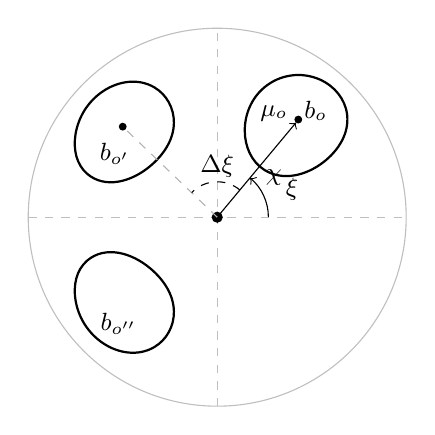
\begin{tikzpicture}[scale=1.0]
\begin{scope}[shift={(7.5,-5)}]
  \draw[thin, gray!50] (0,0) circle (2.4);
  \draw[thin, gray!50, dashed] (-2.4,0) -- (2.4,0);
  \draw[thin, gray!50, dashed] (0,-2.4) -- (0,2.4);
  \filldraw (0,0) circle (1.8pt);
  \draw[thick, closed hobby] plot coordinates {
    (-1.65, -0.55) (-0.85, -0.65) (-0.55, -1.20) (-0.80, -1.65)
    (-1.45, -1.60) (-1.80, -1.05)};
  \node at (-1.25, -1.35) {\small $b_{o''}$};
  \draw[thick, closed hobby] plot coordinates {
    (0.60, 0.60) (1.35, 0.70) (1.65, 1.30) (1.30, 1.75)
    (0.60, 1.65) (0.35, 1.10)};
  \node at (1.25, 1.35) {\small $b_{o}$};
  \filldraw (1.03, 1.24) circle (1.2pt);
  \draw[thick, closed hobby] plot coordinates {
    (-1.65, 0.55) (-0.85, 0.65) (-0.55, 1.20) (-0.80, 1.65)
    (-1.45, 1.60) (-1.80, 1.05)};
  \node at (-1.30, 0.80) {\small $b_{o'}$};
  \filldraw (-1.20, 1.15) circle (1.2pt);
  \draw[->, thin] (0,0) -- (1.00, 1.20);
  \node at (0.72, 0.50) {\small $\chi$};
  \node at (0.72, 1.32) {\small $\mu_o$};
  \draw[thin, gray!60, dashed] (0,0) -- (-1.20, 1.15);
  \draw[->, thin] (0.65, 0) arc (0:50:0.65);
  \node at (0.95, 0.35) {\small $\xi$};
  \draw[thin, dashed] (0,0) ++(50:0.45) arc (50:136:0.45);
  \node at (0, 0.65) {\small $\Delta \xi$};
\end{scope}
\end{tikzpicture}%
}
\par\vspace{10mm}
\caption{}
\label{fig:geo-schematic}
\end{subfigure}
\hfill
\begin{subfigure}[b]{0.37\textwidth}
\centering
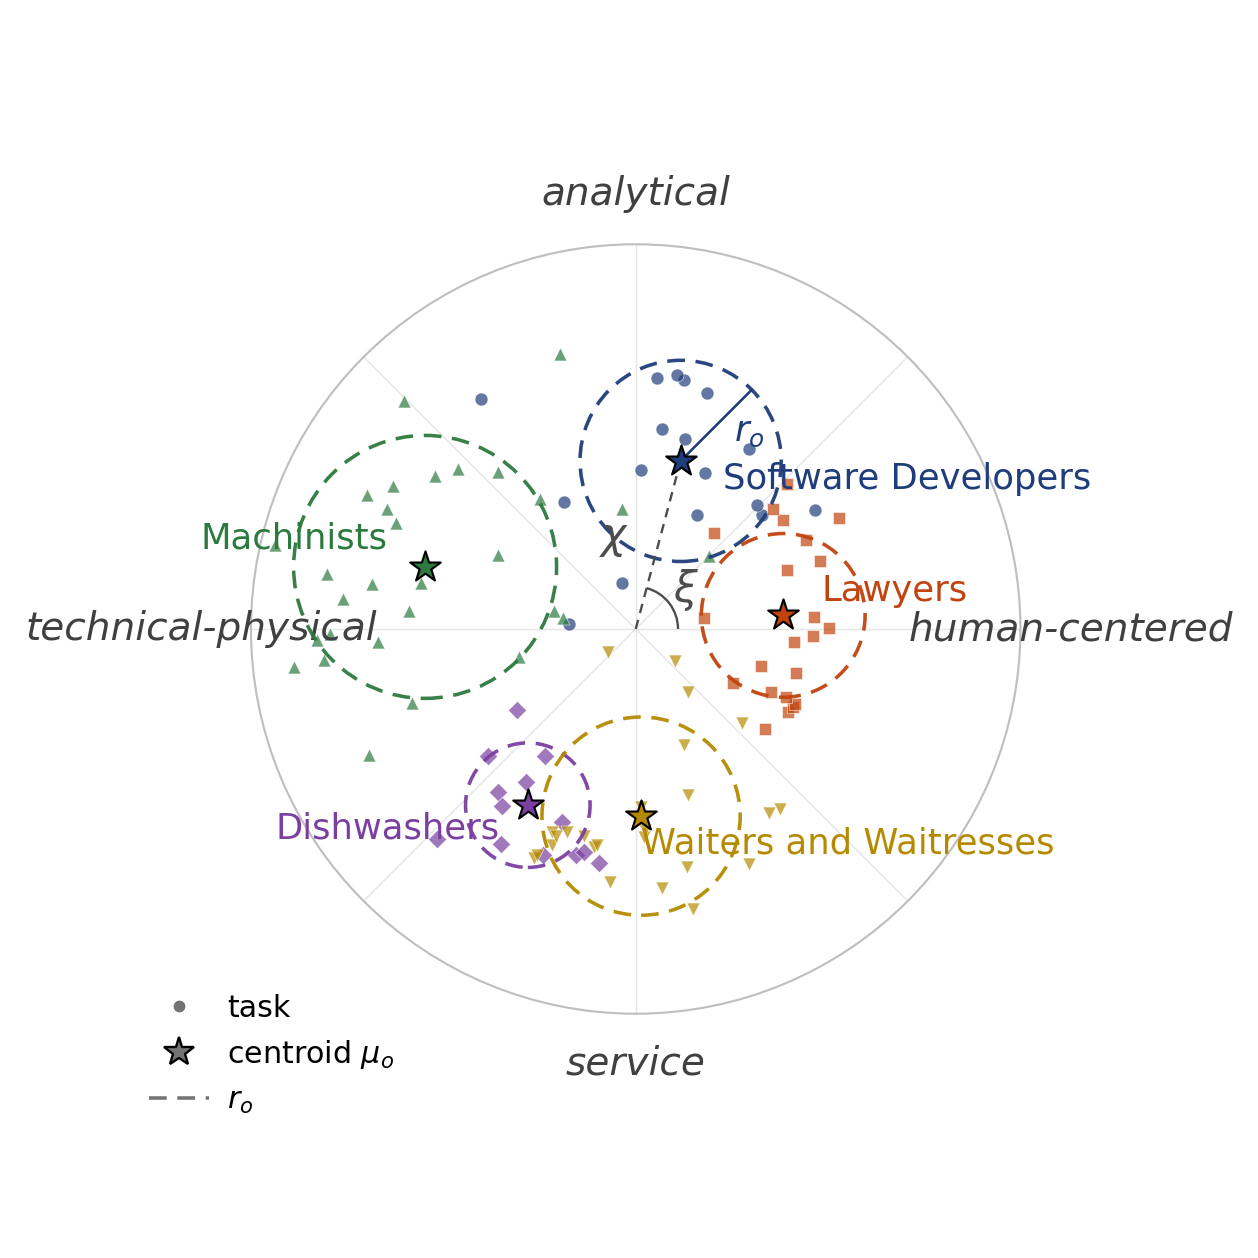
\includegraphics[width=\textwidth]{bundle_examples.png}
\caption{}
\label{fig:geo-bundles}
\end{subfigure}
\hfill
\begin{subfigure}[b]{0.37\textwidth}
\centering
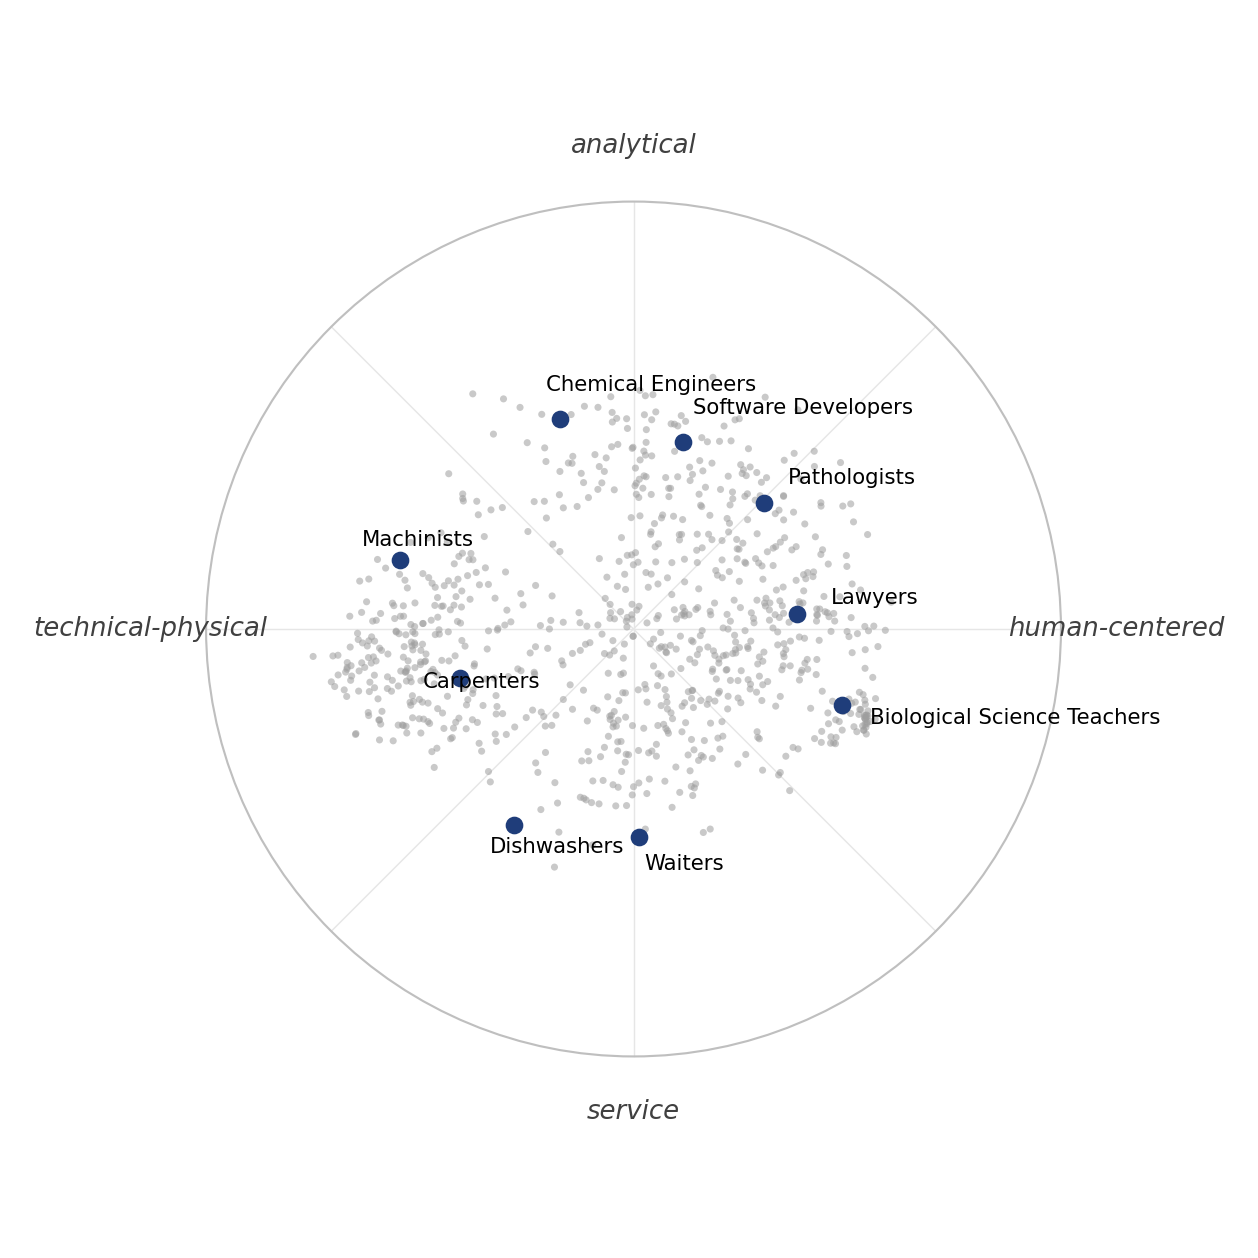
\includegraphics[width=\textwidth]{geometry_map.png}
\caption{}
\label{fig:geo-map}
\end{subfigure}
\caption{The geometry of work. (a) The abstract model of
\textcite{storck2026geometry}: occupations are bundles of tasks on the
polar disk, $b_o$, $b_{o'}$, $b_{o''}$ three bundles with centroids
$\mu_o$; $\xi$ is the angular domain of a centroid, $\Delta\xi$ the
angular separation of two occupations, and $\chi$ the radial specificity.
(b) Five occupations opened as bundles of their tasks: each point is a
task, the star the bundle centroid $\mu_o$, and the dashed circle the
task radius $r_o$, the root-mean-square spread of the bundle around its
centroid rather than an enclosing boundary; Software Developers carries
the coordinate marks $\chi$, $\xi$ and $r_o$. (c) The occupational
centroids of the coordinate universe (grey, 878 occupations;
Section~\ref{sec:frozen-inputs}) with the four directional poles and the
same five example occupations; the rim is the task boundary $\chi=1$.}
\label{fig:geometry-map}
\end{figure}

A task is a unit of work activity that produces output, and a capability
is the stock a worker draws on to perform one \parencite{autor2013a}.
The disk carries tasks. The capabilities that occupations hold are a
separate object on a plane of their own
(Section~\ref{sec:implementation-plane-price}), and the two meet at the
gate that decides whether an occupation can take up a task it has never
performed.

The geometry matters because technologies act on tasks rather than on
occupations as indivisible units. A technology may affect part of an
occupation's bundle while leaving the rest intact. The relevant unit of
exposure is therefore the task location, and the relevant unit of
worker consequence is the rewritten occupational bundle.

The disk has a fixed compass. The east holds human-centered work:
instruction, communication, advice. The north holds analytical work:
research and investigation. The west holds technical-physical work:
mechanical and manual execution. The south holds service work: direct
service and operational support. Tasks near the origin are generic
activities found in many occupations, such as organizing or
documenting; tasks near the rim are domain-specific. The radial
coordinate $\chi$ measures this specificity, and an occupation deep in
a direction is one whose tasks are both specific and aligned.

Panel~(c) of Figure~\ref{fig:geometry-map} places five familiar
occupations on the disk. Lawyers ($5^\circ$) sit in the interpersonal
east and Software Developers ($75^\circ$) in the analytical north.
Machinists ($164^\circ$) occupy the technical-physical west, and
Dishwashers ($239^\circ$) and Waiters ($272^\circ$) the service south.
Throughout the paper, ``the socio-cognitive
north'' refers to the analytical-interpersonal arc from east to north,
``the manual west'' to the technical-physical direction, and ``the
service south'' to the service direction.

Panel~(b) of Figure~\ref{fig:geometry-map} opens the same five
occupations and shows the tasks behind each centroid. Within a bundle
the angle sorts tasks by kind. The Software Developers bundle runs from
client consultation on its human-centered edge, through the analysis
and system design that form its deep core, to shallow installation work
reaching toward the manual west. Lawyers split into an advisory arc
leaning north and a representation arc leaning toward the service side,
neither radially deep: broad judgment rather than narrow
specialization. Machinists span the widest and deepest arc, from
service-leaning setup through a technical core of machining and
diagnosis to an analytical testing edge. Dishwashers occupy a short arc
of one kind, self-contained manual operations whose depth the service
direction does not reward, and Waiters combine service-technical
preparation with the more specific customer interaction.
Appendix~\ref{app:bundle-examples} reproduces the panel with every task
numbered and lists the task statements behind the numbers.

The geometry also matters because the labour market does not price the
space uniformly. The return to depth is directional. Depth in the
socio-cognitive direction is rewarded. In the technical-physical west it
is worth close to nothing, and in the service south it is priced
against: a worker whose service tasks are specific is paid less than one
whose service tasks are generic. This directional wage
structure is estimated in \textcite{storck2026geometry}; Section~\ref{sec:price-field}
recasts it as a price field over the space. It is what allows the model to
distinguish between reinstatement that restores high-priced work and
reinstatement that restores low-priced work.

Because direction sorts tasks by kind, the same kind of work recurs
across occupations at the same place on the disk. Conferring, analyzing
and drafting sit in the core of Software Developers, in the advisory arc
of Lawyers and at the coordinating edge of Machinists. Cleaning, moving
and stocking sit in both service occupations. A technology defined by
where it acts cuts across occupations at a location rather than along the
occupational boundary, and the same technology lands in the deep core of
one bundle and on the shallow edge of another. Where a task sits on the
disk shapes how the market prices it. Whether a technology reaches it is a
separate question, one that turns on the centre and reach of the
technology, and Section~\ref{sec:technology-model} makes it precise.


%% ============================================================
\section{The Price of Work as a Field}
\label{sec:price-field}
%% ============================================================

\textcite{storck2026geometry} estimate a directional wage structure on
the disk: across occupations, the return to specificity is a single
first harmonic of direction, positive toward the analytical north, close
to zero along the east-west axis, and negative toward the service south.
That is a statement about
occupations, observed at their centroids. This paper lifts it to a
statement about locations: the market pays a price $\Pi(\mathbf{r})$
for a unit of work performed at $\mathbf{r}$, and the wage of an
occupation is the price of the work its bundle contains. The lift is
what lets technologies, which act on tasks rather than on occupations,
meet the reward structure of the labour market pointwise. This section
constructs the field, grounds it in the capability content of the
space, and states the sense in which it is an equilibrium object;
Section~\ref{sec:centroids-bundles} validates the lift from centroids
to bundles.

\subsection{The capability plane}
\label{sec:capability-plane}

The price field is grounded in a structural regularity of the
occupational geometry. The capability content of work is, to first
order, organized by a two-dimensional plane in capability space:
\begin{equation}
  v_o
  =
  \bar v
  +
  \chi_o
  \bigl(
    \cos\xi_o\,u_1
    +
    \sin\xi_o\,u_2
  \bigr)
  +
  \varepsilon_o,
  \label{eq:capability-plane}
\end{equation}
where $v_o$ is the capability profile of occupation $o$, $\bar v$ is
the mean profile, and $u_1,u_2$ are the two poles of the plane. The disk
is the polar representation of this plane: $\xi$ is phase and $\chi$ is
amplitude.

Under this structure, distance in task space is interpretable as
distance in capability space, and capability requirements can be read as
fields over the disk. For each capability cluster $k$,
\begin{equation}
  q_k(\xi,\chi)
  =
  \bar v_k
  +
  \chi
  \bigl(
    u_{1,k}\cos\xi
    +
    u_{2,k}\sin\xi
  \bigr).
  \label{eq:capability-field}
\end{equation}
The clusters are the four directional families of O*NET descriptors
identified in \textcite{storck2026geometry}: social-cognitive skills
(S1), technical-physical skills (S2), social-cognitive abilities (A1),
and technical-physical abilities (A2). S1 and A1 peak in the north and
east, S2 in the west and northwest, A2 in the south and west. The
market prices S1 strongly and S2 weakly; A1 and A2 carry no wage
premium once the others are held fixed
(Section~\ref{sec:gate-wedge}).

The empirical implementation tests this postulate directly, on O*NET
capability descriptors that do not enter the construction of the task
coordinates (Section~\ref{sec:implementation-plane-price}).
Higher-order structure is measured as texture and carried in sensitivity
runs, not as part of the core theory.

\subsection{The directional price field}
\label{sec:directional-price}

If capability content is locally planar and capabilities are priced by
a linear functional, then the log price of work is affine in the
capability content of its location:
\[
  \ln \Pi(\mathbf{r})
  =
  \kappa
  +
  \sum_k p_k q_k(\mathbf{r}).
\]
Under the capability plane this implies a first-harmonic directional
depth return. We carry the empirical reduced form as
\begin{equation}
  \ln \Pi(\mathbf{r})
  =
  m_0 + m_1\cos\xi + m_2\sin\xi
  +
  \chi
  \bigl(
    m_3 + m_4\cos\xi + m_5\sin\xi
  \bigr).
  \label{eq:price-field}
\end{equation}
The depth interaction is the theoretical object: it is what makes
depth valuable in some directions and not in others
(Figure~\ref{fig:price-field}).

The derivation restricts this reduced form in two ways, and the
estimates split on them. A capability plane priced by a linear
functional produces no direction-free return to depth, and none is
found: $m_3 = -0.065$, with a standard error of $0.090$. It produces no
level harmonic either, and one survives: a level gradient of amplitude
$0.21$ pointing toward $25^\circ$, carried by $m_1 = 0.192$ with a
standard error of $0.048$. The depth interaction is therefore the part
of the field the microfoundation delivers, and the level terms carry
measured structure outside the exact plane. The fitted depth return
points due north ($89.5^\circ$, amplitude $0.89$) and is positive
between $4^\circ$ and $175^\circ$. It pays $+0.83$ at due north and
$-0.96$ at due south, so specificity in the service direction is priced
against rather than merely unrewarded, and the occupations that absorb
displaced labour in Section~\ref{sec:cognitive-case} lie in that half
of the disk.

The coefficients are estimated once on the occupational wage
cross-section and then held fixed under technology shocks. This is a
deliberate partial-equilibrium choice. The technology model below asks
how a given price structure mediates automation and reinstatement. It
does not re-solve the full assignment of workers and tasks after the
shock.

The reduced form has a structural reading.
Appendix~\ref{app:assignment} reads $\Pi$ as the price surface of a
multidimensional assignment equilibrium in the sense of
\textcite{lindenlaub2017}, in which occupations are capability types
and task demand is CES over locations, and tests that reading on the
frozen inputs. No observed wage enters the computation, so agreement
with the estimated field is a test rather than a fit. Uniform demand
recovers the field's shape but only a quarter of its directed gradient;
a single cognitive demand shifter recovers both. That is the sense in
which the field is an equilibrium object, and what the comparative
statics below hold fixed.

The step from occupational wages to task-location prices is testable.
The field is estimated at occupational centroids, where wages are
observed, but the model prices an occupation as the integral of the
field over its task bundle:
\begin{equation}
  w_o
  =
  \int \Pi(\mathbf{r})\,b_o(\mathbf{r})\,d\mathbf{r}.
  \label{eq:wage-bundle}
\end{equation}
Empirically, bundle-integrated wages reproduce observed wages about as
well as centroid evaluation, which licenses operating the field at the
task level.

\begin{figure}[!htbp]
\centering
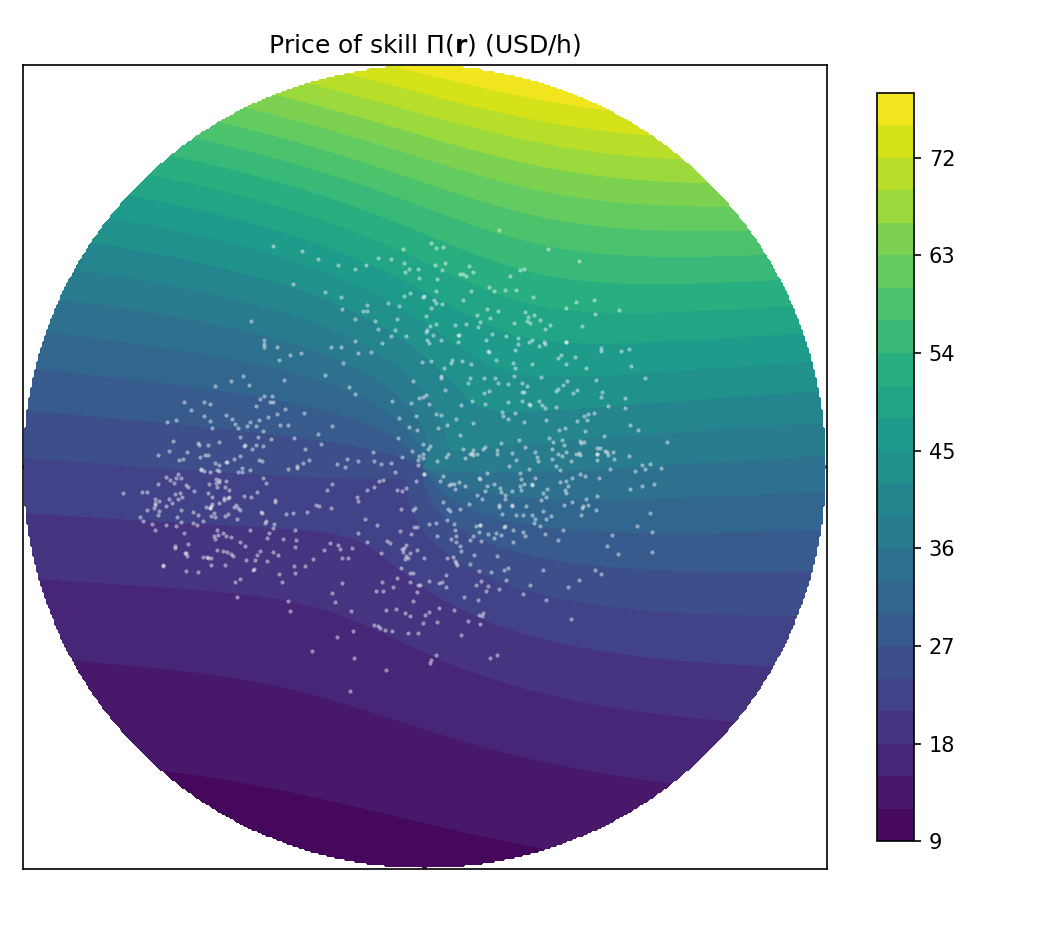
\includegraphics[width=0.8\textwidth]{price_field_map.png}
\caption{The price of skill $\Pi(\mathbf{r})$ over the task disk. The
return to depth is a single first harmonic pointing due north: it is
$+0.83$ at due north, close to zero along the east-west axis, and
$-0.96$ at due south.}
\label{fig:price-field}
\end{figure}


\section{Technology Fields and Task-Bundle Rewriting}
\label{sec:technology-model}
%% ============================================================

This section introduces the paper's central object: the technology
field, a representation of a technology over the task space of
\textcite{storck2026geometry}. The construction is best read against
the one-dimensional model it generalises. \textcite{acemoglu2018race}
order tasks on an interval. Capital can produce every task up to a
moving threshold, and each newly created task enters at the top of the
index, so displacement and reinstatement both act at the two ends of a
line segment. Adoption itself is already economic in that model: an
automatable task goes to capital only where doing so is cheaper. Two
further steps, however, rest on the shape of the line. Comparative
advantage is monotone in the task index, so the newest task is by
definition the task labour is relatively best at, and a ceiling on the
accumulated capital ensures that this task is performed by labour
\parencite{acemoglu2018race}. Newly created tasks that capital would
win are acknowledged and left outside the analysis
\parencite{acemoglu2019automation}.

In two dimensions, each of these devices acquires empirical content.
The top of the index becomes the boundary of a technology field. The
monotone comparative advantage becomes the estimated field
$\Pi(\mathbf{r})$, which orders work by what the market pays for it.
The capital ceiling becomes a price gate applied pointwise, so whether
labour keeps a newly created task is settled location by location, and
the tasks capital wins are counted rather than excluded. The line
gives new work a single place to appear; the disk gives it a
full circle around the field. Which occupations end up holding the new
work stops being fixed by construction and becomes the outcome the
model must deliver. Once occupations are task bundles, reinstatement
must clear labour demand, prices, and capability constraints before it
reaches a worker. That question is what the second dimension opens,
and answering it occupies the rest of the paper.

A technology is represented as an effectiveness field over task space:
\begin{equation}
  \phi_K(\mathbf{r})
  =
  A_K
  \exp
  \left[
    -
    \frac{1}{2}
    \left(
      \frac{\|\mathbf{r}-p_K\|}{z_K}
    \right)^2
  \right],
  \label{eq:phi-K}
\end{equation}
where $p_K$ is the centre of the field, $z_K$ its reach, and $A_K$ its
amplitude. A narrow field represents a specialized technology; a broad
field represents a more general-purpose technology.
Figure~\ref{fig:field-schematic} draws the object, against the set
representation it generalises and on the disk it operates on.

\begin{figure}[!htbp]
\centering
\begin{subfigure}[b]{0.46\textwidth}
\centering
\resizebox{\textwidth}{!}{%
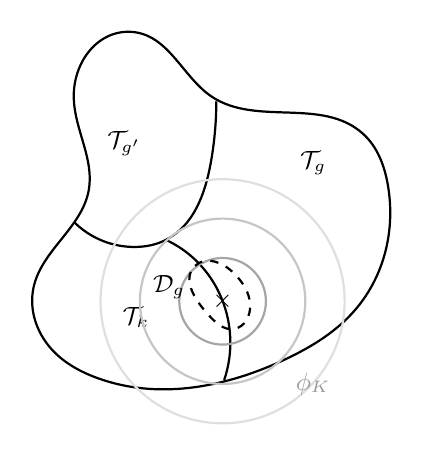
\begin{tikzpicture}[scale=1.0]
  %% A&R set representation (traced from Acemoglu & Restrepo 2022),
  %% with the technology field overlaid.
  \draw[thick, closed hobby] plot coordinates {
    (0.00, 1.18) (0.70, 2.41) (0.51, 3.57) (1.26, 4.42)
    (2.26, 3.60) (4.18, 3.13) (4.50, 2.47) (4.10, 0.91)
    (3.19, 0.26) (0.77, 0.04) (0.22, 0.40)
  };
  \draw[thick, hobby] plot coordinates {
    (2.32, 3.54) (2.25, 2.76) (1.68, 1.78) (1.30, 1.69) (0.52, 2.00)
  };
  \draw[thick, hobby] plot coordinates {
    (1.68, 1.78) (2.07, 1.51) (2.39, 1.03) (2.42, 0.00)
  };
  \node at (1.15, 3.0) {\small $\mathcal{T}_{g'}$};
  \node at (3.55, 2.75) {\small $\mathcal{T}_g$};
  \node at (1.30, 0.80) {\small $\mathcal{T}_k$};
  %% field contours: phi_K is graded around a centre and indifferent
  %% to the set boundaries
  \draw[gray!25, thick] (2.40, 1.00) circle (1.55);
  \draw[gray!45, thick] (2.40, 1.00) circle (1.05);
  \draw[gray!70, thick] (2.40, 1.00) circle (0.55);
  \node at (2.40, 1.00) {\small $\times$};
  \node[gray!80] at (3.55, -0.05) {\small $\phi_K$};
  %% the automation region: a level set of the field
  \draw[thick, dashed, closed hobby] plot coordinates {
    (2.05, 1.45) (2.55, 1.35) (2.75, 0.95) (2.55, 0.65) (2.20, 0.85)
  };
  \node at (1.72, 1.18) {\small $\mathcal{D}_g$};
\end{tikzpicture}%
}
\caption{}
\label{fig:field-set}
\end{subfigure}
\hfill
\begin{subfigure}[b]{0.50\textwidth}
\centering
\resizebox{\textwidth}{!}{%
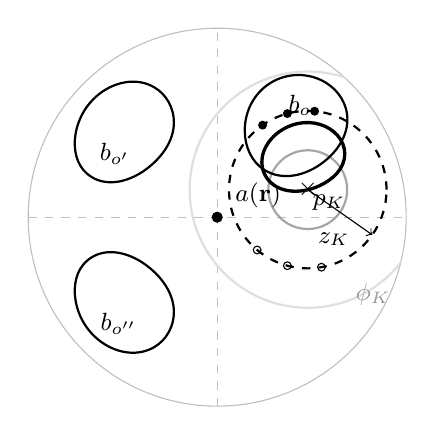
\begin{tikzpicture}[scale=1.0]
  \draw[thin, gray!50] (0,0) circle (2.4);
  \draw[thin, gray!50, dashed] (-2.4,0) -- (2.4,0);
  \draw[thin, gray!50, dashed] (0,-2.4) -- (0,2.4);
  \filldraw (0,0) circle (1.8pt);
  %% field contours and seeding ring, clipped to the disk
  \begin{scope}
    \clip (0,0) circle (2.4);
    \draw[gray!25, thick] (1.15, 0.35) circle (1.50);
    \draw[gray!70, thick] (1.15, 0.35) circle (0.50);
    \draw[thick, dashed] (1.15, 0.35) circle (1.00);
  \end{scope}
  \node at (1.15, 0.35) {\small $\times$};
  \node at (1.42, 0.18) {\small $p_K$};
  \draw[->, thin] (1.15, 0.35) -- ({1.15+1.00*cos(-35)}, {0.35+1.00*sin(-35)});
  \node at (1.48, -0.28) {\small $z_K$};
  \node[gray!80] at (1.98, -0.98) {\small $\phi_K$};
  %% operated region a(r): offset from the field's own contours toward
  %% dear work
  \draw[very thick, closed hobby] plot coordinates {
    (0.60, 0.55) (1.30, 0.40) (1.62, 0.80) (1.30, 1.18) (0.78, 1.08)
  };
  \node at (0.52, 0.28) {\small $a(\mathbf{r})$};
  %% bundles (Figure 1a)
  \draw[thick, closed hobby] plot coordinates {
    (-1.65, -0.55) (-0.85, -0.65) (-0.55, -1.20) (-0.80, -1.65)
    (-1.45, -1.60) (-1.80, -1.05)};
  \node at (-1.25, -1.35) {\small $b_{o''}$};
  \draw[thick, closed hobby] plot coordinates {
    (0.60, 0.60) (1.35, 0.70) (1.65, 1.30) (1.30, 1.75)
    (0.60, 1.65) (0.35, 1.10)};
  \node at (1.05, 1.42) {\small $b_{o}$};
  \draw[thick, closed hobby] plot coordinates {
    (-1.65, 0.55) (-0.85, 0.65) (-0.55, 1.20) (-0.80, 1.65)
    (-1.45, 1.60) (-1.80, 1.05)};
  \node at (-1.30, 0.80) {\small $b_{o'}$};
  %% seed on the ring: filled where a bundle can bind, open where none
  %% reaches
  \filldraw ({1.15+1.00*cos(105)}, {0.35+1.00*sin(105)}) circle (1.4pt);
  \filldraw ({1.15+1.00*cos(125)}, {0.35+1.00*sin(125)}) circle (1.4pt);
  \filldraw ({1.15+1.00*cos(85)}, {0.35+1.00*sin(85)}) circle (1.4pt);
  \draw ({1.15+1.00*cos(230)}, {0.35+1.00*sin(230)}) circle (1.4pt);
  \draw ({1.15+1.00*cos(255)}, {0.35+1.00*sin(255)}) circle (1.4pt);
  \draw ({1.15+1.00*cos(280)}, {0.35+1.00*sin(280)}) circle (1.4pt);
\end{tikzpicture}%
}
\caption{}
\label{fig:field-disk}
\end{subfigure}
\caption{The technology field. (a) The task space of
\textcite{acemoglu2022tasks}, partitioned into sets assigned to factor
categories, with an automation region $\mathcal{D}_g$ moving tasks from
labour to capital, and the field $\phi_K$ of eq.~\eqref{eq:phi-K} laid
over it. The partition carries no metric, so $\mathcal{D}_g$ is a
region without a centre or a reach; under the field it becomes a level
set of a graded effectiveness that has both. (b) The same object on
the disk of Figure~\ref{fig:geometry-map}. Effectiveness falls with
distance from the centre $p_K$ (grey contours). The operated region
$a(\mathbf{r})$ (solid) is where the price gate of
Section~\ref{sec:operated-share} is crossed, offset from the field's
own contours toward dear work. The gradient peaks on the ring at
radius $z_K$ (dashed), where new tasks are seeded
(Section~\ref{sec:reinstatement}). The field cuts inside the bundle
$b_o$; $b_{o'}$ and $b_{o''}$ lie beyond its reach. Seed on the ring
near $b_o$ can bind (filled); seed on the arc no bundle reaches stays
unbound (open).}
\label{fig:field-schematic}
\end{figure}

The circular form is a primitive of the model, as the ordered interval is
a primitive of the one-dimensional framework. Neither is a claim about
the shape of real technologies, and the calibration of
Section~\ref{sec:technology-calibration} therefore asks for the best circular
field the exposure surface supports, not the best field. A richer
shape nests the circle and so fits better by construction: an
anisotropic field with a full covariance, estimated on the same
task-level exposure surface, raises the fit from $R^2=0.25$ to $0.27$.
The question the simplification has to answer is whether the results
depend on it. Under the anisotropic field the seeding density is a
substantially different object, with a rank correlation of $0.65$ against
the circular field's over the model grid, and yet every quantity this
paper reports moves by less than one point: the labour share by $0.5$
points, the unbound share by $1.0$, the reinstatement gap by $0.02$, and
the firm-location enrichment of Section~\ref{sec:check-newwork} by
$0.01$. The reported quantities are integrals of the seeded density
against the price field and the attachment gate, and the integrals are
insensitive to a shape the density is not.

The field does not mean that a whole occupation is automated. At each
task location, the technology can bear some micro-tasks and not others.
The economic question is whether capital is the cheaper producer of
those micro-tasks.

\subsection{The operated share}
\label{sec:operated-share}

Let $s_K \in [0,1]$ denote the replacing character of the technology.
The main simulations take $s_K=1$. Capital performs work at
$\mathbf{r}$ at effective cost
\[
  \frac{R}{s_K\phi_K(\mathbf{r})},
\]
where $R$ is the rental cost of capital. Labour performs the same work
at price $\Pi(\mathbf{r})$. Capital is the cheaper producer where
\begin{equation}
  s_K\phi_K(\mathbf{r})
  >
  \frac{R}{\Pi(\mathbf{r})}.
  \label{eq:regime-shift}
\end{equation}
Within the reach of the technology, this condition is crossed first
where labour is highly priced. The model therefore separates technical
exposure, $\phi_K$, from economic incidence, $a(\mathbf{r})$.

Because a location contains a continuum of micro-tasks, the condition is
smoothed into an operated share:
\begin{equation}
  a(\mathbf{r})
  =
  \frac{
    1
  }{
    1+
    \exp
    \left(
      -
      \frac{
        s_K\phi_K(\mathbf{r}) - R/\Pi(\mathbf{r})
      }{\tau}
    \right)
  },
  \label{eq:soft-switch}
\end{equation}
where $\tau$ is the width of the adoption margin. As $\tau \to 0$, the
share approaches a sharp partition; for positive $\tau$, it is the
fraction of micro-tasks at a location that capital bears.

Displacement is loss of paid human task content. For occupation $o$,
the displaced share is
\begin{equation}
  D_o
  =
  \int b_o(\mathbf{r})\,a(\mathbf{r})\,d\mathbf{r}.
  \label{eq:displaced}
\end{equation}
An occupation may therefore experience substantial displacement even if
no spatial region is fully automated. The margin cuts inside the bundle.

\subsection{Reinstatement as boundary task creation}
\label{sec:reinstatement}

Reinstatement returns a fraction $\gamma$ of displaced task mass as new
tasks. The question is where these tasks appear and which occupations
can bind them.

New tasks are seeded where the technology field changes most rapidly:
\begin{equation}
  \|\nabla\phi_K(\mathbf{r})\|
  =
  \frac{1}{z_K^2}
  \|\mathbf{r}-p_K\|
  \phi_K(\mathbf{r}).
  \label{eq:gradient-phi}
\end{equation}
This gradient peaks at distance $z_K$ from the technology centre. Let
\[
  \hat g(\mathbf{r})
  =
  \frac{
    \|\nabla\phi_K(\mathbf{r})\|
  }{
    \int \|\nabla\phi_K(\mathbf{r})\|\,d\mathbf{r}
  }
\]
be the normalized boundary density and let
\[
  M = \gamma \Delta\Gamma^D
\]
be the seeded task mass, where
\[
  \Delta\Gamma^D = \sum_o L_o D_o.
\]
The seeded density is
\[
  \zeta(\mathbf{r}) = M\hat g(\mathbf{r}).
\]

A seed does not automatically become human work. It survives as human
work only to the extent that labour remains the cheaper producer at its
location. The surviving seed density is therefore
\[
  \zeta(\mathbf{r})(1-a(\mathbf{r})),
\]
while
\[
  \zeta(\mathbf{r})a(\mathbf{r})
\]
is captured by capital.

\subsection{The deficit gate}
\label{sec:deficit-gate}

A surviving seed can attach to an existing occupation only if the
occupation and the task fit each other. The fit is measured in priced
capabilities. The capability deficit of occupation $o$ at location
$\mathbf{r}$ is
\begin{equation}
  \delta_o(\mathbf{r})
  =
  \sum_{k\in\mathcal K}
  v_k
  \max(q_k(\mathbf{r})-q_{o,k},0),
  \label{eq:deficit}
\end{equation}
where $q_k(\mathbf{r})$ is the requirement of capability cluster $k$ at
location $\mathbf{r}$, $q_{o,k}$ is occupation $o$'s capability content,
and $v_k$ is the corresponding component of the price functional. In
the main implementation, $\mathcal K$ contains the priced clusters. The
corresponding surplus is
$\bar\delta_o(\mathbf{r})=\sum_{k\in\mathcal K}
v_k\max(q_{o,k}-q_k(\mathbf{r}),0)$, the priced capability the
occupation holds in excess of what the task requires.

Readiness to attach the task is
\begin{equation}
  e_o(\mathbf{r})
  =
  \exp\!\bigl[
    -\bigl(\delta_o(\mathbf{r})
    +\lambda_{\mathrm{over}}\,\bar\delta_o(\mathbf{r})\bigr)/\ell
  \bigr]
  \,
  \exp\bigl(-\|\mathbf{r}-\mu_o\|/\rho\bigr),
  \label{eq:attachment}
\end{equation}
where $\ell$ is a global acquisition scale,
$\lambda_{\mathrm{over}}$ weights the surplus, and $\rho$ sets the
attachment locality around the occupation's centroid. The form
penalizes deficit and surplus together because being able to do a task
and becoming its home are different questions. The deficit records
what the occupation would have to acquire; the surplus records how far
the task sits below the occupation's priced level, and without the
penalty an over-qualified generalist far from its core would bind seed
as if it were home territory. The locality term keeps attachment near
the bundle the occupation actually performs.

Setting $\lambda_{\mathrm{over}}=0$ and $\rho\to\infty$ gives the
one-sided limit
\begin{equation}
  e_o(\mathbf{r})
  =
  \exp[-\delta_o(\mathbf{r})/\ell],
  \label{eq:readiness}
\end{equation}
in which only deficits bar attachment. The limit is useful for
intuition --- an occupation can always absorb a task that uses less of
a capability it already holds --- but eq.~\eqref{eq:attachment} is the
form the model carries. Total attachment capacity at
a location is
\[
  C(\mathbf{r})
  =
  \sum_o L_o e_o(\mathbf{r}).
\]
The bound share of surviving seed mass is
\[
  \Phi(C) = \frac{C}{1+C}.
\]
Occupation $o$ receives reinstated density
\begin{equation}
  \iota_o(\mathbf{r})
  =
  \zeta(\mathbf{r})
  (1-a(\mathbf{r}))
  \Phi(C(\mathbf{r}))
  \frac{
    L_o e_o(\mathbf{r})
  }{
    C(\mathbf{r})
  }.
  \label{eq:reinstated}
\end{equation}

The price gate and the deficit gate act in series. The first decides
whether a seed survives as human work. The second decides which
occupation, if any, can bind it.

\subsection{Unbound tasks and candidate occupations}
\label{sec:unbound}

Not all surviving seed attaches. The unbound density is
\begin{equation}
  u(\mathbf{r})
  =
  \zeta(\mathbf{r})
  (1-a(\mathbf{r}))
  [1-\Phi(C(\mathbf{r}))].
  \label{eq:unbound}
\end{equation}
It collects the new tasks that survive capital but that no existing
occupation can perform. The density is not an agent or a nascent
occupation; it maps mismatch.

Each seeded location therefore has three possible fates:
\[
  a(\mathbf{r}) \quad \text{captured by capital,}
\]
\[
  (1-a(\mathbf{r}))\Phi(C(\mathbf{r}))
  \quad \text{bound by existing occupations,}
\]
\[
  (1-a(\mathbf{r}))[1-\Phi(C(\mathbf{r}))]
  \quad \text{left unbound.}
\]
These shares exhaust the seeded mass.

Unbound mass is a location on the disk that no occupation reaches. It
has no counterpart in a representation where every point is an
occupation \parencite{yamaguchi2012, neffke2013, alabdulkareem2018},
because there is nowhere in such a space for work that nobody does.
Where unbound mass is diffuse, it represents friction. Where it
clusters, it marks a candidate region for occupational emergence.
Whether such a region is an opportunity or merely low-paid residual work
depends on the price field. Unbound mass in a high-$\Pi$ region is
latent skilled work awaiting a bearer; unbound mass in a low-$\Pi$
region is closer to precarious task spillage.

\subsection{The bundle operator}
\label{sec:bundle-operator}

The two gates rewrite the occupation. The post-technology bundle is
\begin{equation}
  b_o^{\text{post}}(\mathbf{r})
  =
  b_o(\mathbf{r})(1-a(\mathbf{r}))
  +
  \frac{\iota_o(\mathbf{r})}{L_o}.
  \label{eq:bundle-operator}
\end{equation}
The occupation is not abolished. Its paid task content is redrawn:
automation strips operated content, and reinstatement adds the seeded
content the occupation can bind.

The operator does not preserve bundle mass. Its integral is
\[
  \int b_o^{\text{post}}(\mathbf{r})\,d\mathbf{r}
  =
  1 - D_o + B_o/L_o,
  \qquad
  B_o=\int\iota_o(\mathbf{r})\,d\mathbf{r}.
\]
We do not renormalize the bundle. Renormalizing would assume that freed
time is reallocated proportionally across the remaining tasks; here the
mass deficit is the labour released to the worker layer of
Section~\ref{sec:employment-demand}.

The re-pricing of the bundle at the frozen field is
\begin{equation}
  \Delta w_o
  =
  \int
  \Pi(\mathbf{r})
  \left[
    -b_o(\mathbf{r})a(\mathbf{r})
    +
    \frac{\iota_o(\mathbf{r})}{L_o}
  \right]
  d\mathbf{r}.
  \label{eq:wage-change}
\end{equation}
The first term removes paid content, typically the high-priced content
the gate takes first. The second adds new human task content, but only
where the deficit gate permits attachment. Reinstatement therefore
carries a downward wage bias when it strips dear work and refills with
cheap work. Equation~\eqref{eq:wage-change} is the object taken to the
wage data in Section~\ref{sec:directional-check}.

%% ============================================================
\section{Employment and Mobility}
\label{sec:employment-demand}
%% ============================================================

The task layer rewrites bundles. The worker layer determines how labour
is reallocated after the rewrite. We close the model as a static
spatial-sorting equilibrium and read technology effects as comparative
statics between the pre-technology and post-technology rest points.

\subsection{Task-work and place output}
\label{sec:taskwork}

The market structure is stated once and used throughout. Each location
$\mathbf{r}$ hosts a local product assembled from its micro-task
continuum in fixed proportions. Human task work at $\mathbf{r}$ costs
$\Pi(\mathbf{r})$. Capital is supplied elastically at rental $R$ and is
paid its cost, $R/(s_K\phi_K(\mathbf{r}))$ per unit of task work; it
retains no quasi-rent.

The human part of occupation $o$'s coverage is
\[
  h_o(\mathbf{r}) = b_o^{\text{post}}(\mathbf{r}),
\]
and the capital part is
\[
  k_o(\mathbf{r}) = b_o(\mathbf{r})a(\mathbf{r}).
\]
Total task-work at location $\mathbf{r}$ is
\begin{equation}
  n(\mathbf{r})
  =
  \sum_o L_o
  \bigl[
    h_o(\mathbf{r}) + k_o(\mathbf{r})
  \bigr]
  =
  \sum_o L_o b_o(\mathbf{r})
  +
  \sum_o \iota_o(\mathbf{r}).
  \label{eq:taskwork-density}
\end{equation}

Two components of seeded mass stay outside
eq.~\eqref{eq:taskwork-density}. Unbound tasks have no bearer and
produce nothing. Capital-captured seeds are new capital-run production;
pricing them requires re-solving the field and is deferred with the rest
of the closure. Only bound seed enters the frozen-field economy. The
fate accounting of Section~\ref{sec:unbound} records all three.

Place output is
\begin{equation}
  V(\mathbf{r})
  =
  \Pi(\mathbf{r})
  n(\mathbf{r})^\beta,
  \qquad \beta\in(0,1).
  \label{eq:place-output}
\end{equation}
The congestion exponent $\beta<1$ is local capacity; its rent
$(1-\beta)V$ accrues to a fixed local factor and stays outside the wage
analysis.

Automation lowers the marginal cost of the local product where capital
bears the task, but revenue at a location does not respond to that
saving here: place output is valued at the frozen price field. Whether
the cost saving expands output and draws labour back in, or contracts it
and releases labour, is the demand channel
\parencite{bessen2019demand}. It acts on a margin this paper does not
study, and holding it shut is what isolates the question the paper does
ask, which is who performs the work and what it pays.

\subsection{Occupation values}
\label{sec:occupation-values}

The value of occupation $o$ is
\begin{equation}
  W_o
  =
  \beta
  \int
  h_o(\mathbf{r})
  \Pi(\mathbf{r})
  n(\mathbf{r})^{\beta-1}
  d\mathbf{r}.
  \label{eq:occ-value}
\end{equation}
Occupation values are coupled because many occupations cover the same
task locations. When workers move into an occupation, they raise density
where that occupation operates and reduce marginal value through
congestion.

Human task work is paid its marginal value product,
eq.~\eqref{eq:occ-value}. Pricing uses cost; payment uses marginal
value. The two are not tied by a zero-profit condition here, because
that condition re-solves the price field. The frozen-field model keeps
this seam visible and defers the closure.

The paper carries three wage objects. The bundle wage
$w_o=\int\Pi\,b_o$ prices a bundle at the frozen field and is used for
cross-sectional levels. The occupation value $W_o$ adds congestion and
is what workers sort on. The bundle wage change
$\Delta w_o$ of eq.~\eqref{eq:wage-change} is the operator's gross
re-pricing of the bundle and is the object taken to the data in
Section~\ref{sec:directional-check}. They agree on direction and differ
in what they hold fixed.

\subsection{Spatial re-sorting}
\label{sec:sorting}

Labour re-sorts from the pre-technology distribution. The mobility cost
between two occupations is proportional to their distance in task space,
task distance in the sense of \textcite{gathmann2010}:
\[
  d(j,o)=\|\mu_j-\mu_o\|.
\]
The probability that a worker originating in occupation $j$ moves to
occupation $o$ is
\begin{equation}
  P_{j\to o}
  =
  \frac{
    \exp[(W_o+\alpha_o-c_m\,d(j,o))/\nu]
  }{
    \sum_{o'}
    \exp[(W_{o'}+\alpha_{o'}-c_m\,d(j,o'))/\nu]
  },
  \label{eq:transition-probability}
\end{equation}
where $c_m$ governs mobility cost, $\nu$ logit smoothness, and the
constants $\alpha_o$ absorb occupational attributes the value $W_o$
does not carry: amenities, institutional wage setting, entry
requirements. Employment
in occupation $o$ is then
\begin{equation}
  L_o
  =
  \sum_j L_j^0 P_{j\to o}.
  \label{eq:equilibrium}
\end{equation}
This is a fixed point because $W_o$ depends on $n(\mathbf{r})$, which
depends on the employment vector $L$. Total labour is fixed; allowing
aggregate labour supply to respond to total value is a later extension.

The constants anchor the model to the data. They are set once, by
requiring that observed employment $L^0$ be the fixed point of the
sorting map with no technology present. Writing
$v_o=\exp(\alpha_o/\nu)$, the requirement is that the destination
marginals of the zero-technology transition matrix reproduce $L^0$, a
balancing problem with a unique solution up to the additive constant
that cancels in the logit; a Sinkhorn iteration recovers it. Without
the constants the observed allocation is not a rest point of the
logit, and a solved equilibrium mixes the technology's effect with a
baseline relocation that has nothing to do with the technology. With
them, $L-L^0$ is the technology's own employment response. The
mobility scales come from the same baseline: $\nu$ is one standard
deviation of the zero-technology occupation value, and a median-length
move costs one logit unit.
The sorting layer is reduced-form by design: a static allocation rule,
rather than a search or matching model, that makes mobility costly in
task-space distance and lets congestion close the equilibrium.

\subsection{Labour share}
\label{sec:labour-share}

Let
\[
  H(\mathbf{r})
  =
  \sum_o L_o h_o(\mathbf{r})
\]
be human task-work. The labour share of variable task-work income is
\begin{equation}
  \Lambda
  =
  \frac{
    \int
    \Pi(\mathbf{r})
    H(\mathbf{r})
    n(\mathbf{r})^{\beta-1}
    d\mathbf{r}
  }{
    \int
    \Pi(\mathbf{r})
    n(\mathbf{r})^\beta
    d\mathbf{r}
  }.
  \label{eq:labour-share}
\end{equation}
The share does not scale with the congestion exponent. Since
$\int\Pi H n^{\beta-1} = \int \Pi n^{\beta}(H/n)$, $\Lambda$ is the
weighted mean of the local human share of task work, with weights
proportional to $\Pi n^{\beta}$, so $\beta$ enters only through those
weights and the multiplicative $\beta$ of eq.~\eqref{eq:occ-value}
cancels. It does not cancel from the distribution of wages across
occupations: where displaced labour crowds in, the density $n$ rises
and the return $n^{\beta-1}$ falls, so re-sorting bends the effective
wage down in the receiving directions and up in the vacated ones. The
aggregate is silent on this because it nets to zero in $\Lambda$; the
cross-section of occupation wages is not. Section~\ref{sec:cognitive-case}
reads this second channel off the calibrated case.
Automation lowers the
share where the operated share rises; reinstatement raises it only where
new human task-work binds. $\Lambda$ weights human task work by the
local value of task work. It records who performs the valued work; the
full income statement of a location, with capital cost, congestion rent
and consumer gain, belongs to the deferred closure. The object is
internal to the model. It is one before the shock because no capital
bears any task then, so a post-shock value of $\Lambda$ measures how
much of a fully mature technology's task income capital takes in this
economy. It is not the labour share of national income and is not
comparable to it.

%% ============================================================
\section{Empirical Implementation and Calibration}
\label{sec:implementation}
%% ============================================================

This section measures the frozen objects used by the model and
calibrates the technology fields it operates. The theory objects are
the capability plane and the price functional. The measurement objects
are their estimated coordinates, the bundle-pricing validation, and the
family wage wedge. The simulation primitives are the technology and
economy parameters varied or held fixed in Section~\ref{sec:cognitive}.

\subsection{Data and frozen inputs}
\label{sec:frozen-inputs}

All inputs are vendored from a pinned commit of the
\textcite{storck2026geometry} repository. The frozen inputs are the
occupation and task coordinates, O*NET task relevance ratings, OEWS
median hourly wages, education levels, capability cluster intensities,
and raw O*NET Skills and Abilities descriptors.

Four occupation samples appear in the paper, and each use is fixed
here. The coordinate universe contains $878$ occupations and is the
sample of every capability-side estimation and of the geometry figures.
Of these, $849$ occupations carry observed OEWS employment and
constitute the simulation economy of Sections~\ref{sec:employment-demand}
and~\ref{sec:cognitive}. Of these, $785$ occupations carry matched median
wages and form the estimation sample of the price field and the
mediation regression. Finally, $725$ occupations ($640$ distinct SOC
codes) carry a median wage in both OEWS vintages and form the sample of
Section~\ref{sec:directional-check}. The attrition is data
availability at each step, not selection by the model. The task
universe contains $17{,}606$ statements, of which $17{,}549$
($99.7$~percent) join the exposure data of
Section~\ref{sec:technology-calibration} on Task ID.

\subsection{Capability plane and price field}
\label{sec:implementation-plane-price}

The capability plane is the second of the two objects of
Section~\ref{sec:geometry}, the stock rather than the activity
\parencite{autor2013a}. It is estimated from descriptor deviations and
tested against the task disk. The leading two components account for roughly
three quarters of the capability deviation variance and align strongly
with the disk coordinates. The cluster fields $q_k(\xi,\chi)$ are then
estimated by OLS on occupation-level capability intensities
(Table~\ref{tab:plane-coefficients-new}).

The price field is estimated by OLS of log median hourly wage on the
polar regressors in eq.~\eqref{eq:price-field}, on the $785$
occupations of the wage sample. The estimation replicates the wage
equation of \textcite{storck2026geometry} exactly on the frozen
inputs, and is printed here because the model operates on it. The
estimated field, with HC3 standard
errors in parentheses, is
\begin{equation}
\ln \Pi(\mathbf{r}) =
\underset{(0.036)}{3.420}
+ \underset{(0.048)}{0.192}\,\cos\xi
+ \underset{(0.051)}{0.089}\,\sin\xi
+ \chi\bigl(\underset{(0.090)}{-0.065}
+ \underset{(0.112)}{0.008}\,\cos\xi
+ \underset{(0.134)}{0.891}\,\sin\xi\bigr),
\label{eq:price-estimates}
\end{equation}
with $R^2 = 0.523$. The isotropic depth term is indistinguishable from
zero ($p = 0.47$), and the depth return is carried by a single strong
first harmonic of amplitude $0.891$ peaking at $89.5^\circ$, in the
socio-cognitive north: depth pays only through its interaction with
direction. A second-harmonic test balanced with level harmonics does
not reject the single first harmonic of the depth return ($p = 0.44$);
the remaining higher-order structure is mainly a level effect, not an
additional depth-pricing mechanism. The surface is also not a snapshot
artefact: re-estimated on the 1999, 2003, and 2007 OEWS cross-sections
carried onto the same coordinates, its peak direction, isotropic term,
and amplitude are stable within one standard error on a constant
occupation set.\footnote{Same specification, historical wages joined
through the SOC 2000--2018 crosswalks. On the balanced code set the
peak direction is $93$--$96^\circ$ across 1999--2007 against $93^\circ$
on the 2023 cross-section, the isotropic term is zero in every vintage,
and the amplitude lies between $0.83$ and $0.96$ with no trend.
Full-sample fits differ across vintages, but the differences are
carried by which occupation codes publish per vintage, not by
repricing.} Estimated sector by sector rather than as a harmonic, the
depth return runs from $+0.93$ in the north to $-1.18$ in the
south-east and traces the fitted first harmonic, and it reproduces the
published sectoral estimates of \textcite{storck2026geometry} on the
frozen inputs to within $0.005$.

\begin{table}[!htbp]
\centering
\caption{Capability plane coefficients, estimated on the full
coordinate universe ($N=878$; wages not required). Each cluster's
requirement field is $q_k=\bar v_k+\chi(u_{1,k}\cos\xi+u_{2,k}\sin\xi)$
(eq.~\eqref{eq:capability-field}); $R^2$ is the two-pole plane fit and
$\Delta R^2$ the gain from adding level harmonics and isotropic depth.}
\label{tab:plane-coefficients-new}
\begin{tabular}{lcccccc}
\toprule
Cluster & $\bar v_k$ & $u_{1,k}$ & $u_{2,k}$ & Pole & $R^2$ & $\Delta R^2$ \\
\midrule
S1 & $2.68$ & $1.09$ & $1.42$ & $52^\circ$ & $0.74$ & $0.001$ \\
S2 & $1.37$ & $-2.22$ & $1.23$ & $151^\circ$ & $0.69$ & $0.008$ \\
A1 & $3.20$ & $0.95$ & $1.31$ & $54^\circ$ & $0.75$ & $0.000$ \\
A2 & $1.57$ & $-1.54$ & $-0.24$ & $189^\circ$ & $0.57$ & $0.009$ \\
\bottomrule
\end{tabular}
\end{table}

\subsection{From centroids to bundles}
\label{sec:centroids-bundles}

The reduced-form step from occupational centroids to task locations is
validated by bundle integration. The bundle-integrated wage
\[
  w_o=\int \Pi(\mathbf{r})b_o(\mathbf{r})d\mathbf{r}
\]
predicts observed wages about as well as evaluating the price field at
the centroid ($R^2=0.51$ against $0.52$ at the centroid; correlation
$0.72$). The centroid figure is the estimation's own in-sample fit,
while the bundle predictor is out of specification, so parity is the
informative outcome (Figure~\ref{fig:field-wages-new}). The Jensen gap between the two is small (mean
$+0.018$). This licenses the model's use of $\Pi$ at task locations.

\begin{figure}[!htbp]
\centering
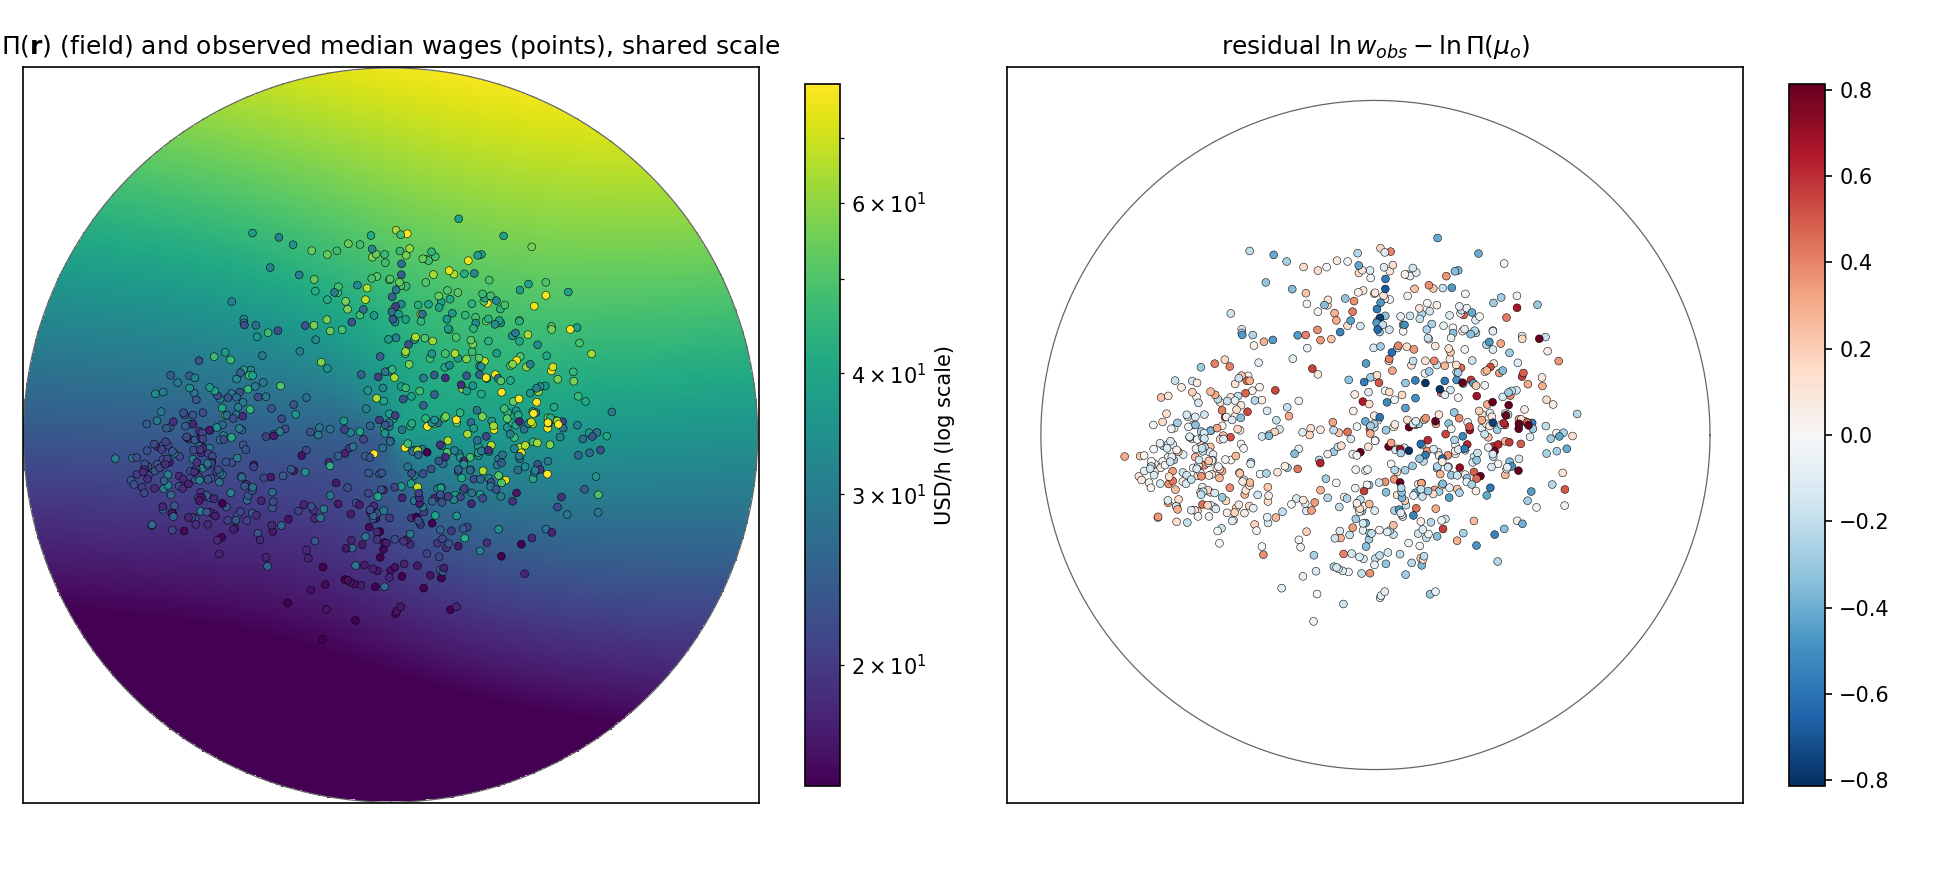
\includegraphics[width=0.8\textwidth]{field_vs_observed_wages.png}
\caption{Bundle-integrated wage against observed wage.}
\label{fig:field-wages-new}
\end{figure}

\subsection{Gate weights and wage wedge}
\label{sec:gate-wedge}

The gate weights $v_k$ are the components of the price functional. They
are estimated by replicating the mediation regression of
\textcite{storck2026geometry} on the wage sample ($N=785$, HC3
standard errors). The gate carries the sign restriction $v_k \geq 0$:
a capability enters the deficit only if the market prices it. The
estimates are $v_{S1} = 0.328$ ($0.065$) and $v_{S2} = 0.049$
($0.021$); the ability clusters carry negative or negligible estimates
and are excluded by the restriction, so the priced set is
$K = \{S1, S2\}$, with S1 dominant and S2 smaller.

The price field does not price occupations exactly, and the residual
carries information the gate can use. Let
\[
  \omega_o
  =
  \ln w_{\mathrm{obs},o}
  -
  \ln w_{\mathrm{bundle},o}
\]
be the amount by which occupation $o$ is paid above or below the value
of its own bundle at the field, and let the family wage wedge
$\omega_g$ be the job-family mean of that residual. Family means absorb
$0.30$ of the occupation-level residual variance, and the wedge runs
from $-0.26$ log points in Personal Care and Service to $+0.37$ in
Management, which is the shape institutional wage setting would leave.
The wedge is measured once on the frozen inputs and held fixed under
the technology shock. Where it is used, it enters the adoption gate and
nothing else, through
\[
  \Pi_{\mathrm{eff}}(\mathbf{r}) = e^{\omega_g}\,\Pi(\mathbf{r}),
\]
so that capital compares its cost to what the work is paid rather than
to what the field says the work is worth. The ordering of displacement
barely moves under the wedge (rank correlation $0.99$ in $D_o$), while
the level shifts for the families furthest from the field, Management
most. Every headline result is reported without the wedge, and
Section~\ref{sec:cognitive-case} reports the mechanism with it.

\subsection{Locating a technology field}
\label{sec:technology-calibration}

A technology field is located by least squares on an exposure surface:
the four parameters of eq.~\eqref{eq:phi-K} are fitted to a measure of
which work the technology can bear. The rule is the same for every field
the paper carries. What differs is the substrate the exposure is
measured on, and whether the surface has an interior peak.

Identification turns on the second. A Gaussian's shape is carried by its
curvature, and curvature lives near the peak; far out in the tail a tall
narrow field and a low broad one are hard to tell apart. A surface whose
exposure turns over inside the occupied region pins centre, reach and
amplitude separately. A surface that rises monotonically toward the
periphery does not: the fitted centre goes to the edge of the support,
and what the data pin is the field's value where work is, not the
field's shape. Both cases arise below, and each field's subsection
reports which it is. The field's value is the object the operated share
reads, so the results survive the weaker case. The seeded density is a
curvature object and does not survive it, which is what the invariance
check of Section~\ref{sec:technology-model} is for.

The economy parameters are set by explicit rules and held fixed across
scenarios; Table~\ref{tab:economy-parameters} lists them. One rule is
circular by construction and stated as such: the rental cost $R$ is set
so that the gate binds in the calibrated field's core, because an
inoperative technology has no results to report. The level of the
automation cut is therefore not identified, and the $R$ sweep of
Section~\ref{sec:cognitive-case} reports how far it moves with the
gate. Sensitivity of the headline quantities to the remaining
parameters is reported there as well.

\begin{table}[!htbp]
\centering
\caption{Economy parameters. Employment $L$ is normalized to shares
summing to one, so the attachment capacity $C$ in $\Phi(C)=C/(1+C)$ is
of order one. Mobility and anchoring values are set at the
zero-technology baseline.}
\label{tab:economy-parameters}
\begin{tabular}{ll>{\raggedright\arraybackslash}p{8.2cm}}
\toprule
Parameter & Value & Rule \\
\midrule
$R$ & $18$ & the gate binds in the calibrated field's core: capital
cost $R/(s_K\phi_K)\approx30$ at the centre against $\Pi\approx47$;
the gate closes where $s_K\phi_K\Pi<R$ \\
$\tau$ & $0.08$ & width of the adoption margin, eq.~\eqref{eq:soft-switch} \\
$\beta$ & $0.5$ & congestion benchmark; enters $\Lambda$ only through
the weights \\
$\gamma$ & $0.5$ & seeded fraction of displaced mass; swept below \\
$\ell$ & $0.133$ & one within-direction SD of the priced-capability
index gives readiness $e^{-1}$ \\
$\rho,\ \lambda_{\mathrm{over}}$ & $0.5,\ 1$ & attachment locality and
over-qualification weight, eq.~\eqref{eq:attachment} \\
$\nu$ & $16.4$ & one SD of zero-technology occupation value per logit unit \\
$c_m$ & $31.8$ & the median move costs one $\nu$ \\
$\alpha_o$ & balanced & occupation constants; observed employment is the
zero-technology rest point of the sorting map \\
\bottomrule
\end{tabular}
\end{table}

\subsection{Automation waves as technology fields}
\label{sec:automation-waves}

The same calibration locates other technologies, and the exercise shows
what the representation can carry. \textcite{webb2020} builds
occupational exposure to three technologies by matching patent text to
O*NET tasks: industrial robots, software, and machine learning. Fitting
each to the disk, beside the language-model exposure, places four
technologies in one geometry (Table~\ref{tab:webb-fields},
Figure~\ref{fig:webb-fields}). Webb's measures are occupation-level, so
all four are fitted on the occupation substrate here; the cognitive
field's centre reported below ($40^\circ$) is its occupation-substrate
fit, while the analysis uses its task-level calibration of
Table~\ref{tab:technology-calibration-new}.

Read in the order the technologies diffused, the fields sweep across the
space. Industrial robots sit in the technical-physical west, at the
periphery where production and manual work lie, with a narrow reach.
Software sits to the north-west, over routine technical work. Machine
learning, the AI of Webb's patents through about 2018, sits in the
analytical north. Language models sit in the north-east, broad over
high-priced cognitive work. The centres fall in an arc from the physical
west to the cognitive north-east, in the order the waves arrived. This
is the spatial form of the succession of automation technologies
documented by \textcite{acemoglu2020robots} for robots and by
\textcite{autor2003} for computerisation: each wave acts on different
work, and the geometry locates where.

Two of the four fields are localised. The robot field and the
language-model field centre inside the occupied disk, and their reach
follows a concentrated exposure. The software and machine-learning
surfaces are gradients rather than peaks. Exposure rises toward the
north without an interior maximum, so a single field centres at the edge
of the occupied region and its reach is an artefact of that shape.
Webb's machine learning locates AI further north than the language-model
measure and does not coincide with it, which is expected, since
patent-era machine learning and language models are different
technologies acting on different work.

Three limits bound the reading. The chronology is external to the data.
Webb's three measures are built from patents through about 2018, so they
do not date the technologies; the order comes from when each diffused.
The measures do not share a source, since robots, software, and machine
learning are one construction and language models another. And four
fields illustrate the representation, not a temporal law. The robot
field of Section~\ref{sec:robot-field} and the software field are the
two that the analysis uses again, as the placebo of
Section~\ref{sec:check-confound} and as counterfactual fields in
Section~\ref{sec:check-robot-wage}.

\begin{table}[!htbp]
\centering
\caption{The four technology fields fitted on the common occupation
substrate, in the order the technologies diffused. Robots, software, and
machine learning are the patent-based exposures of \textcite{webb2020};
language models are the LLM exposure of \textcite{eloundou2024}. Fit is
the $R^2$ on the between-cell exposure surface; the centre column marks
fields whose centre sits at the edge of the occupied disk (support
$\chi=0.75$). The cognitive field's analysis calibration is the
task-level fit of Table~\ref{tab:technology-calibration-new}.}
\label{tab:webb-fields}
\begin{tabular}{llccccl}
\toprule
Technology & Source & $\xi_K$ & $\chi_K$ & $z_K$ & $R^2$ & Centre \\
\midrule
Industrial robots & Webb      & $207^\circ$ & $0.75$ & $0.50$ & $0.84$ & at edge \\
Software          & Webb      & $146^\circ$ & $0.75$ & $0.80$ & $0.62$ & at edge \\
Machine learning  & Webb      & $108^\circ$ & $0.75$ & $0.70$ & $0.70$ & at edge \\
Language models   & Eloundou  & $40^\circ$  & $0.49$ & $0.57$ & $0.83$ & localised \\
\bottomrule
\end{tabular}
\end{table}

\begin{figure}[!htbp]
\centering
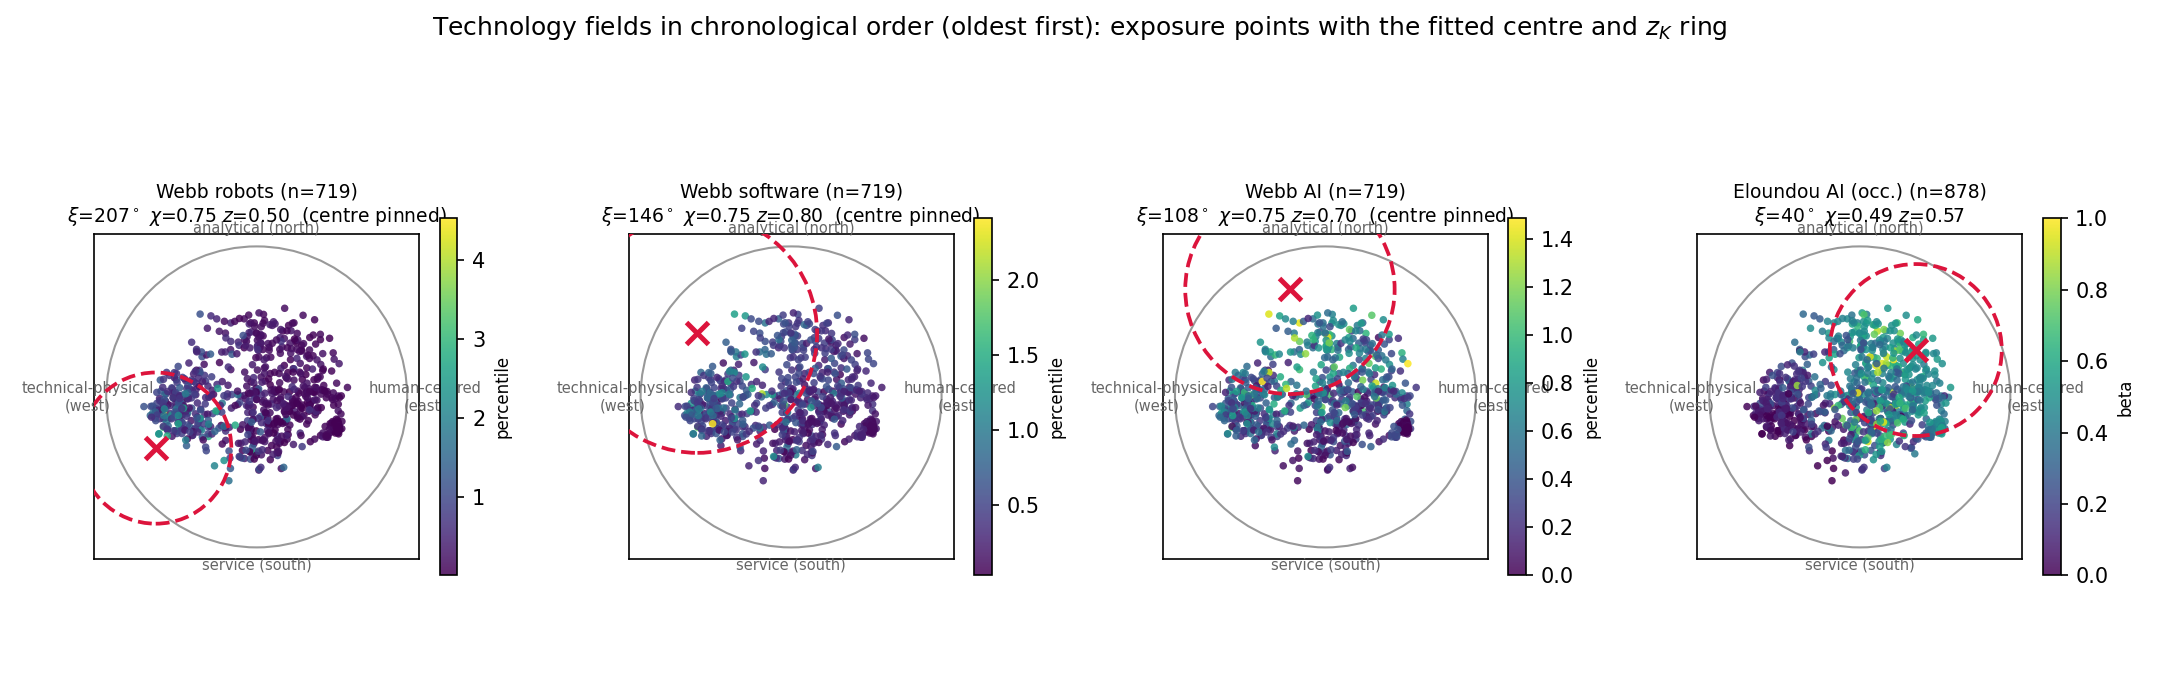
\includegraphics[width=\textwidth]{webb_points_and_rings.png}
\caption{The four technology fields, oldest first. Each panel shows the
occupations coloured by their exposure to one technology, with the
fitted field centre ($\times$) and the $z_K$ ring. Industrial robots,
software, and machine learning are from \textcite{webb2020}; language
models from \textcite{eloundou2024}. The robot and language-model fields
enclose a concentrated exposure; the software and machine-learning
surfaces rise toward the north without an interior peak, so their fitted
centre sits at the edge of the occupied disk.}
\label{fig:webb-fields}
\end{figure}

%% ============================================================
\section{The industrial-robot field}
\label{sec:robot}
%% ============================================================

We run the model twice. The industrial-robot field comes first, because
its scale can be tied to an observed employment moment and its wage
response falls in a window where that response can be identified. The
cognitive field comes second, where neither holds: its scale rests on a
modelling rule, and its wage cross-section cannot discriminate. The two
fields carry different evidence and are treated differently where the
evidence requires it. What is compared across them is the structure of
the result, not its level.

\subsection{Locating and scaling the field}
\label{sec:robot-field}

The industrial-robot field is fitted by the rule of
Section~\ref{sec:technology-calibration} to the occupational robot
exposure of \textcite{webb2020}. The exposure is occupation-level, so
the fit runs on the occupation substrate, not the task substrate.
The fitted field is western, centred at $207^\circ$ in the
technical-physical periphery where production and manual work lie, with
$\chi_K = 0.75$ and reach $z_K = 0.50$, and it reproduces $84$~percent
of the smoothable exposure surface (Figure~\ref{fig:webb-fields}, first
panel).

The centre is a boundary solution, and we report it as one. The
occupation cloud ends at $\chi = 0.752$ and the fitted centre sits on
that edge. Robot exposure rises toward the technical-physical periphery
without turning over inside the occupied region, so the fit has no
interior peak to sit on: two occupations lie within $0.10$ of the fitted
centre, against the $437$ tasks under the cognitive field's. What the
exposure surface pins is the field's value over the region where work
is, and that is the object the operated share reads. Centre and reach
are pinned only jointly, through that value: a field placed further out
with a proportionately longer reach describes the same exposure on the
same occupations, and nothing below distinguishes them. Such a field
would move the seeded density, which is a curvature object, and
Section~\ref{sec:technology-calibration} certifies that the reported
quantities do not move with it.

The amplitude carries the scale, and here the robot field has what the
cognitive field lacks. The fitted amplitude sits on the normalized
exposure scale and has no cost units, so the gate takes its scale from
elsewhere. Rather than a rule, we use a moment: $A_K$ is set by
bisection so that the aggregate displaced task mass $\sum_o L_o D_o$
matches the displacement of \textcite{acemoglu2020robots}, about
$400{,}000$ jobs on a $135$~million base over the diffusion years, a
share of $0.0030$. That returns $A_K = 1.477$ at the $1999$ price field.
Task mass is equated to jobs at the aggregate, and the moment is a net
local-equilibrium employment effect while the model's object is gross
stripped mass, so matching gross to net makes the calibrated field
conservative. Sensitivity at half and double the moment is reported
below.

\subsection{Displacement and the labour share}
\label{sec:robot-equilibrium}

The field is run in its own era. The price field is $\Pi_{1999}$,
employment weights are the $1999$ OEWS levels over $774$ occupations,
and mobility and readiness are set by the committed rules on the era's
own baseline.

Displacement lands where the field is
(Figure~\ref{fig:robot-incidence}, left). The mean displaced bundle share
in the western arc is $0.0136$ against $0.00065$ outside it, a factor of
twenty-one, and the occupations at the top of the list are the ones the
robot literature would name: dredge operators, rail-track equipment
operators, rebar workers, boilermakers and forging machine setters, at
$2.8$ to $3.6$ percent of bundle mass.

\begin{figure}[!htbp]
\centering
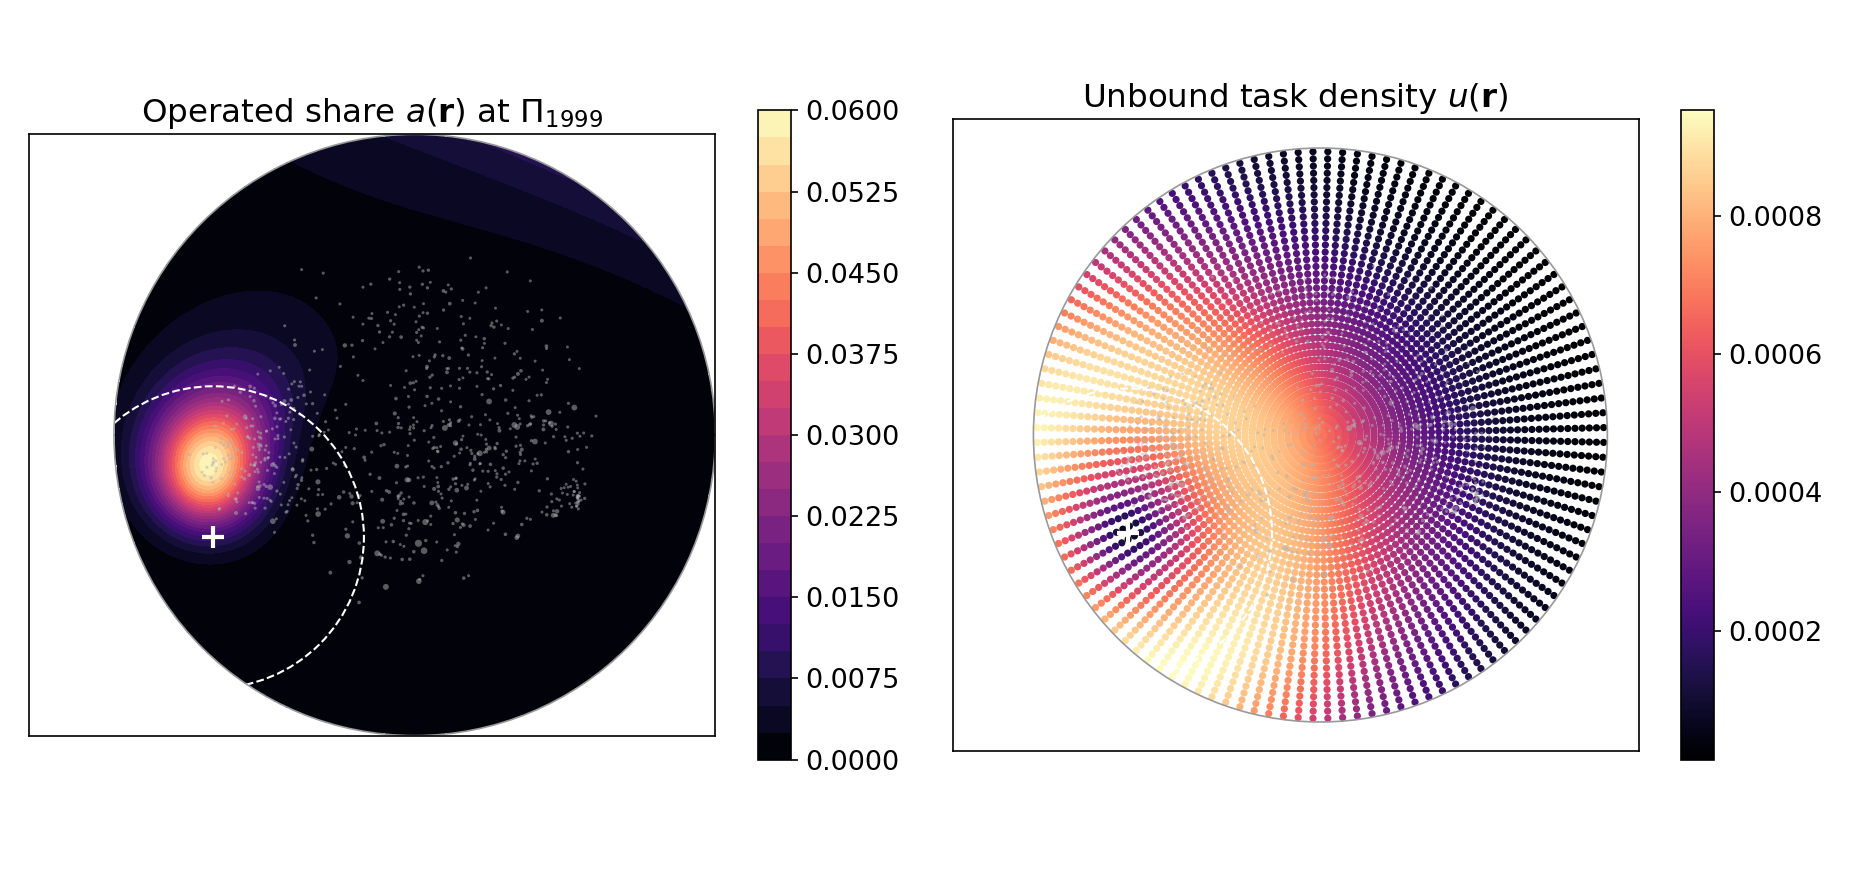
\includegraphics[width=\textwidth]{robot_era_incidence.png}
\caption{Incidence of the calibrated robot field in its own era. Left:
operated share $a(\mathbf{r})$ at $\Pi_{1999}$; grey dots are the 1999
occupation centroids, sized by employment. The gate opens over the
technical-physical west, at the edge of the occupied disk, and
displacement concentrates in the occupations under it. Right: unbound
task density $u(\mathbf{r})$, with the field centre ($+$) and the
seeding ring at $z_K$ (dashed). The seed falls on the outer western
arc, beyond the occupations that could bind it; $93$~percent of it
binds to nobody (Section~\ref{sec:robot-binding}).}
\label{fig:robot-incidence}
\end{figure}

The labour share falls from its pre-technology normalization of one to
$0.9948$ under automation, and reinstatement leaves it at $0.9925$. The
drop is small because the shock is small, and the shock is the one the
robot era delivered: the model was told its size and did not choose it. Reinstatement does not close the gap. Employment moves accordingly
little, relocating $0.11$~percent of mass.

\subsection{Who binds the new work}
\label{sec:robot-binding}

Of the mass the field seeds, $93$~percent survives capital and binds to
no existing occupation (Figure~\ref{fig:robot-incidence}, right). Seven
percent binds. The share is a property of
the geometry rather than of the calibration: it moves by half a point
between half and double the displacement moment, and it is $92.8$
percent at observed employment as well as at solved.

The model does not name the occupations that take up the remainder.
Bound mass $B_o$ is dominated by occupation size, because attachment
capacity is $C(\mathbf{r}) = \sum_o L_o e_o(\mathbf{r})$, capability
weighted by employment, so the largest occupations absorb most of what
binds whatever the technology. The ranking is headed by retail
salespersons, cashiers and baristas, and it is headed by the same
occupations under the cognitive field, whose centre lies in the opposite
half of the disk. Bound mass per worker is flat across the top of the
ranking, a spread of $1.02$ over the top ten. What the model identifies
is how much of the seed binds to nobody. It does not identify a bearer
for the rest, and we do not claim one.

What the unbound mass is worth can be said. It sits at $0.93$ times the
mean price of work in the $1999$ economy, a little below what that
economy paid on average. The reading follows Section~\ref{sec:unbound}:
this is work the field creates that no occupation reaches, and its price
is what separates a skill gap from a wage floor.

\subsection{Where the wage burden falls}
\label{sec:robot-wages}

Occupation wage adjustments decompose exactly into three channels: the
content stripped from the bundle, the congestion induced by the inflow
of freed labour, and the new work the occupation binds. Under the robot
field the employment-weighted means are $-0.0029$ log points of
stripping, a congestion mean of zero against a mean absolute of
$0.0010$, and $+0.0035$ of reinstatement, which is more than stripping
takes.

The decomposition is order-invariant here. Attributing congestion before
stripping rather than after moves the channel magnitudes by under one
percent, against the $54$~percent the cognitive field produces on the
same test. The channels interact through the product of their
magnitudes, and the robot shock is small enough that they barely do.
Order-dependence is a function of shock size, not a defect of the
decomposition, and that is visible only with two shocks of different
size to compare.

Why reinstatement covers stripping here and not under the cognitive
field is a question about prices, and the price field answers it. Within
an occupation, capital takes content dearer than the occupation's own
average, at a ratio of $1.17$; the gate orders locations by price inside
a band of equal effectiveness, and that much is mechanical. Across
occupations the field is nonetheless aimed at cheap work. The content
the robot field takes is priced at $0.83$ times the mean price of work in
its own economy, and the bound work it seeds lands at $0.89$ times that
mean. The exchange is even, at $1.07$, and $1.04$ when the seeded work is
priced at the centroid of the occupation that binds it rather than at its
own location on the disk. The robot wave destroys work worth about what
the work it creates is worth, and no wage burden follows.
Section~\ref{sec:cognitive-case} runs the same three numbers for a field
aimed at the other side of the disk.

\subsection{Against the data}
\label{sec:robot-data}
\label{sec:check-robot-wage}

An occupational wage window can test a wage prediction only if the
prediction is separable from the wage level. Automation targets dear
work, so a field's predicted pressure tends to load on the baseline wage,
and a period in which relative wage growth also loads on the baseline
wage will return a correlation for any such field, real or fictitious.
Section~\ref{sec:cognitive-data} shows that the cognitive wave's own
window fails on exactly this count, and what that costs.

The robot wave's window does not fail on it. Its diffusion years are
covered by a classification-consistent wage window, 1999 to 2007 with
2003 as midpoint, frozen onto the geometry through composed SOC
crosswalks, and the collinearity is absent by measurement: the robot
field's predicted bundle wage pressure at $\Pi_{1999}$ loads on the 1999
wage level at $+0.03$, so the wage level explains none of whatever
correlation appears.

The instrument is the bundle wage pressure $\Delta w_o$ rather than the
directional projection, and the geometry forces the choice. The
projection records the direction a residual centroid moves. A field in
the dear region strips dear content and points residuals down the
gradient; a field in the cheap region strips cheap content and points
residuals up the gradient; and for any single-peaked field the
projection is monotone in position along the gradient axis. In a window
whose wage growth carries a positional trend, the projection therefore
correlates for every field, real or fictitious, with the sign set by
orientation alone. The bundle pressure has no such degeneracy: more
stripped value predicts lower relative wage growth wherever the field
sits.

Table~\ref{tab:wave-window} reports the result. Occupations under
deeper predicted robot pressure saw lower wage growth over 1999--2007
(Spearman $+0.22$, unchanged at $+0.22$ given the baseline wage, and
$+0.21$ on the stable-crosswalk subsample), in both halves of the
window (Figure~\ref{fig:robot-window}). Three counterfactual fields,
each calibrated to the same aggregate displaced mass so that the
comparison is between locations rather than scales, carry the opposite
sign: the cognitive field evaluated before the technology existed
($-0.29$ given the wage level), a rotated robot clone ($-0.22$), and
the software field of Section~\ref{sec:automation-waves} ($-0.12$). Their correlations are the period's
positional growth trend, the cognitive north-east pulling ahead of the
wage level, and their sign is mechanism-inconsistent: their nominally
pressed occupations grew faster. The robot field alone carries the
mechanism's sign.

Running both waves through both windows closes the design. In
2019--2025 the objects behave as Section~\ref{sec:check-confound}
found: the cognitive raw correlation ($+0.42$) collapses given the
baseline wage ($+0.03$), and the robot raw ($-0.20$) is manufactured by
a $+0.31$ loading on the wage level and collapses the same way
($-0.02$). One cell of the four survives conditioning with the
mechanism's sign, the robot in its own window. The scope is that of any
occupational cross-section: robots and import competition pressed the
same western manufacturing arc over these years
\parencite{autor2013china}. A manufacturing-share control meets the
confound directly. Each occupation's manufacturing employment share is
strongly collinear with the predicted pressure (rank correlation
$-0.63$), and the robot correlation survives conditioning on it beside
the wage level, at $+0.20$.\footnote{The share is built from the BLS
industry-specific occupational employment files: employment in NAICS
31--33 over employment across all industries, per SOC-2000 occupation,
May 2003 (the window midpoint), mapped onto the frozen geometry through
the composed crosswalks. The 2002 vintage gives a rank correlation of
$0.98$ with the 2003 shares.} The correlation is therefore not the
manufacturing-wide decline. What the window still cannot separate is
import exposure varying across industries within the manufacturing arc,
so the attribution caveat narrows without closing.

\begin{table}[!htbp]
\centering
\caption{Each wave in each window. Spearman rank correlations between
predicted bundle wage pressure and observed occupational wage growth;
the partial correlation conditions on the rank of the start-of-window
wage level. Within each window both fields are calibrated to the same
aggregate displaced task mass, set by the window's own wave ($N=774$ in
1999--2007, $725$ in 2019--2025).}
\label{tab:wave-window}
\begin{tabular}{lcccc}
\toprule
 & \multicolumn{2}{c}{1999--2007} & \multicolumn{2}{c}{2019--2025} \\
Field & Raw & Partial & Raw & Partial \\
\midrule
Industrial robots & $+0.22$ & $+0.22$ & $-0.20$ & $-0.02$ \\
Cognitive & $-0.38$ & $-0.29$ & $+0.42$ & $+0.03$ \\
\bottomrule
\end{tabular}
\end{table}

\begin{figure}[!htbp]
\centering
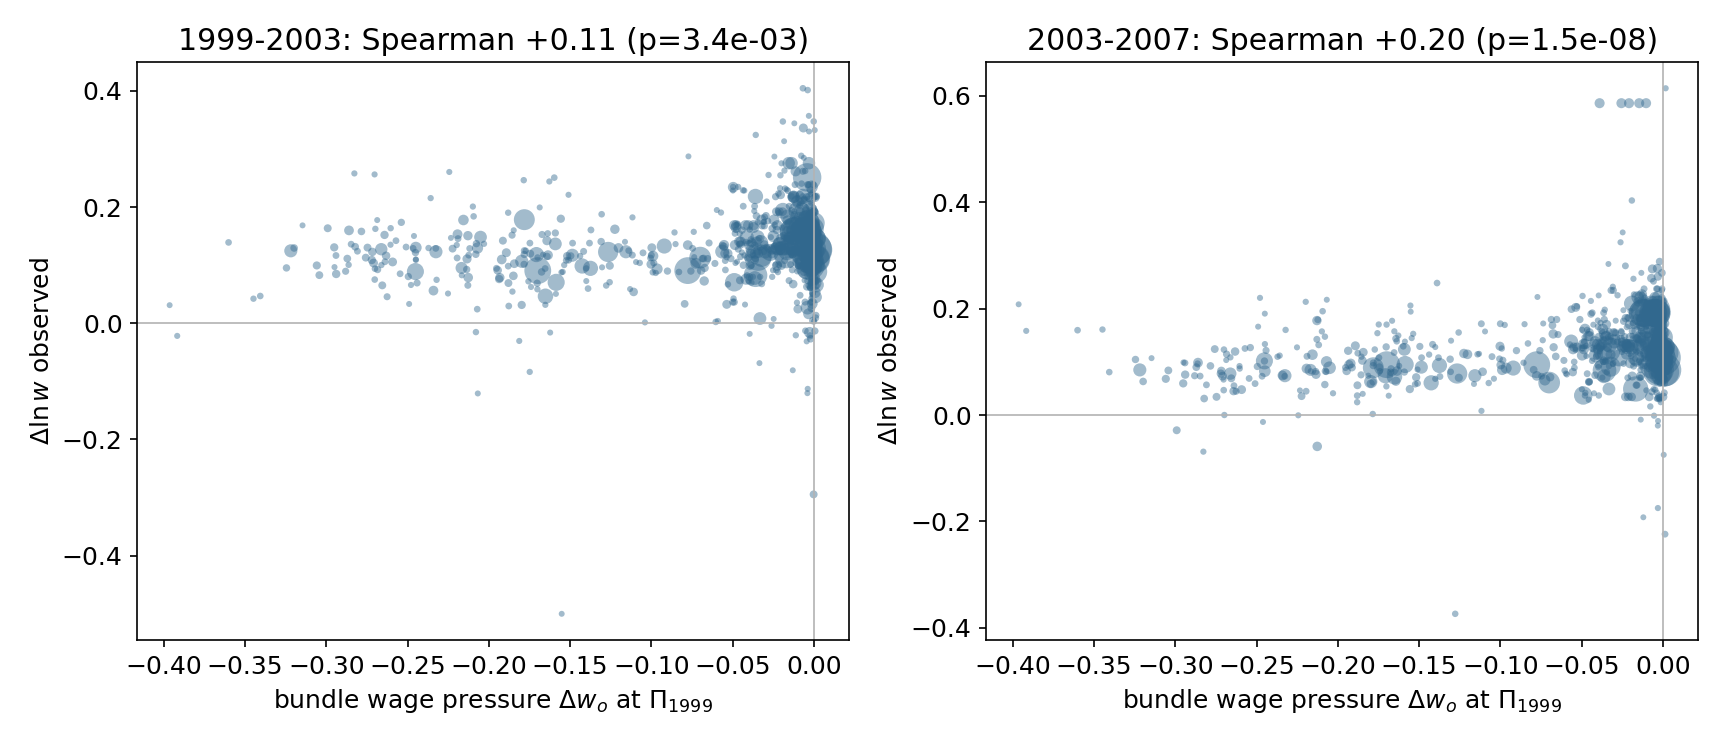
\includegraphics[width=\textwidth]{robot_era_directional.png}
\caption{Predicted bundle wage pressure of the calibrated robot field
at $\Pi_{1999}$ against observed occupational wage growth, in the two
halves of the robot window. Marker size is 1999 employment. The
pressure measure is nearly orthogonal to the wage level, so the raw and
conditioned correlations coincide.}
\label{fig:robot-window}
\end{figure}

%% ============================================================
\section{The cognitive field}
\label{sec:cognitive}
%% ============================================================

The cognitive field is the application. Its scale rests on a modelling
rule and not on a moment, and its wage cross-section falls in a window
where the response cannot be identified, so its levels are read against
the sweeps below and its confrontation with data is the weaker of the
two. What carries across from Section~\ref{sec:robot} is the structure.

\subsection{Locating and scaling the field}
\label{sec:cognitive-field}

The cognitive technology field is calibrated to task-level AI exposure:
each task statement carries the exposure score
$\beta_E = E1 + \tfrac12 E2$ of \textcite{eloundou2024}.
Occupation-level exposure measures exist
\parencite{webb2020,felten2021occupational}; the field is fitted at
the task level because that is where the geometry lives. The scores are
joined to the task coordinates on Task ID ($17{,}549$ of $17{,}606$
statements, $99.7$~percent) and fitted with the Gaussian field in
eq.~\eqref{eq:phi-K}. The fitted field lies in the
socio-cognitive north, with broad reach and moderate amplitude. The
field explains a modest share of task-level exposure ($R^2=0.25$) but
most of the smoothable between-cell exposure surface ($R^2=0.82$).

The modest task-level fit is a property of the rating scale, not of
the field form. The exposure ratings clump at discrete values, so the
between-cell share of the task-level variance --- the smoothable
ceiling for any field --- is $0.30$ on the polar grid, and the single
isotropic Gaussian captures $82$~percent of it. The parameters are
jointly identified: the fitted centre lies inside the occupied disk
($\chi_K = 0.463$ against occupational support $\chi \leq 0.752$), so
the peak amplitude is observed rather than extrapolated from a flank,
and the Gauss--Newton normal matrix is well conditioned (condition
number $30$, with correlation $-0.30$ between $z_K$ and $A_K$).
Figure~\ref{fig:exposure-fit-new} shows the fitted field against the
exposure surface. Directional structure the isotropic field misses is
carried as texture; a richer $\phi_K$ is an extension, not a repair.

\begin{figure}[!htbp]
\centering
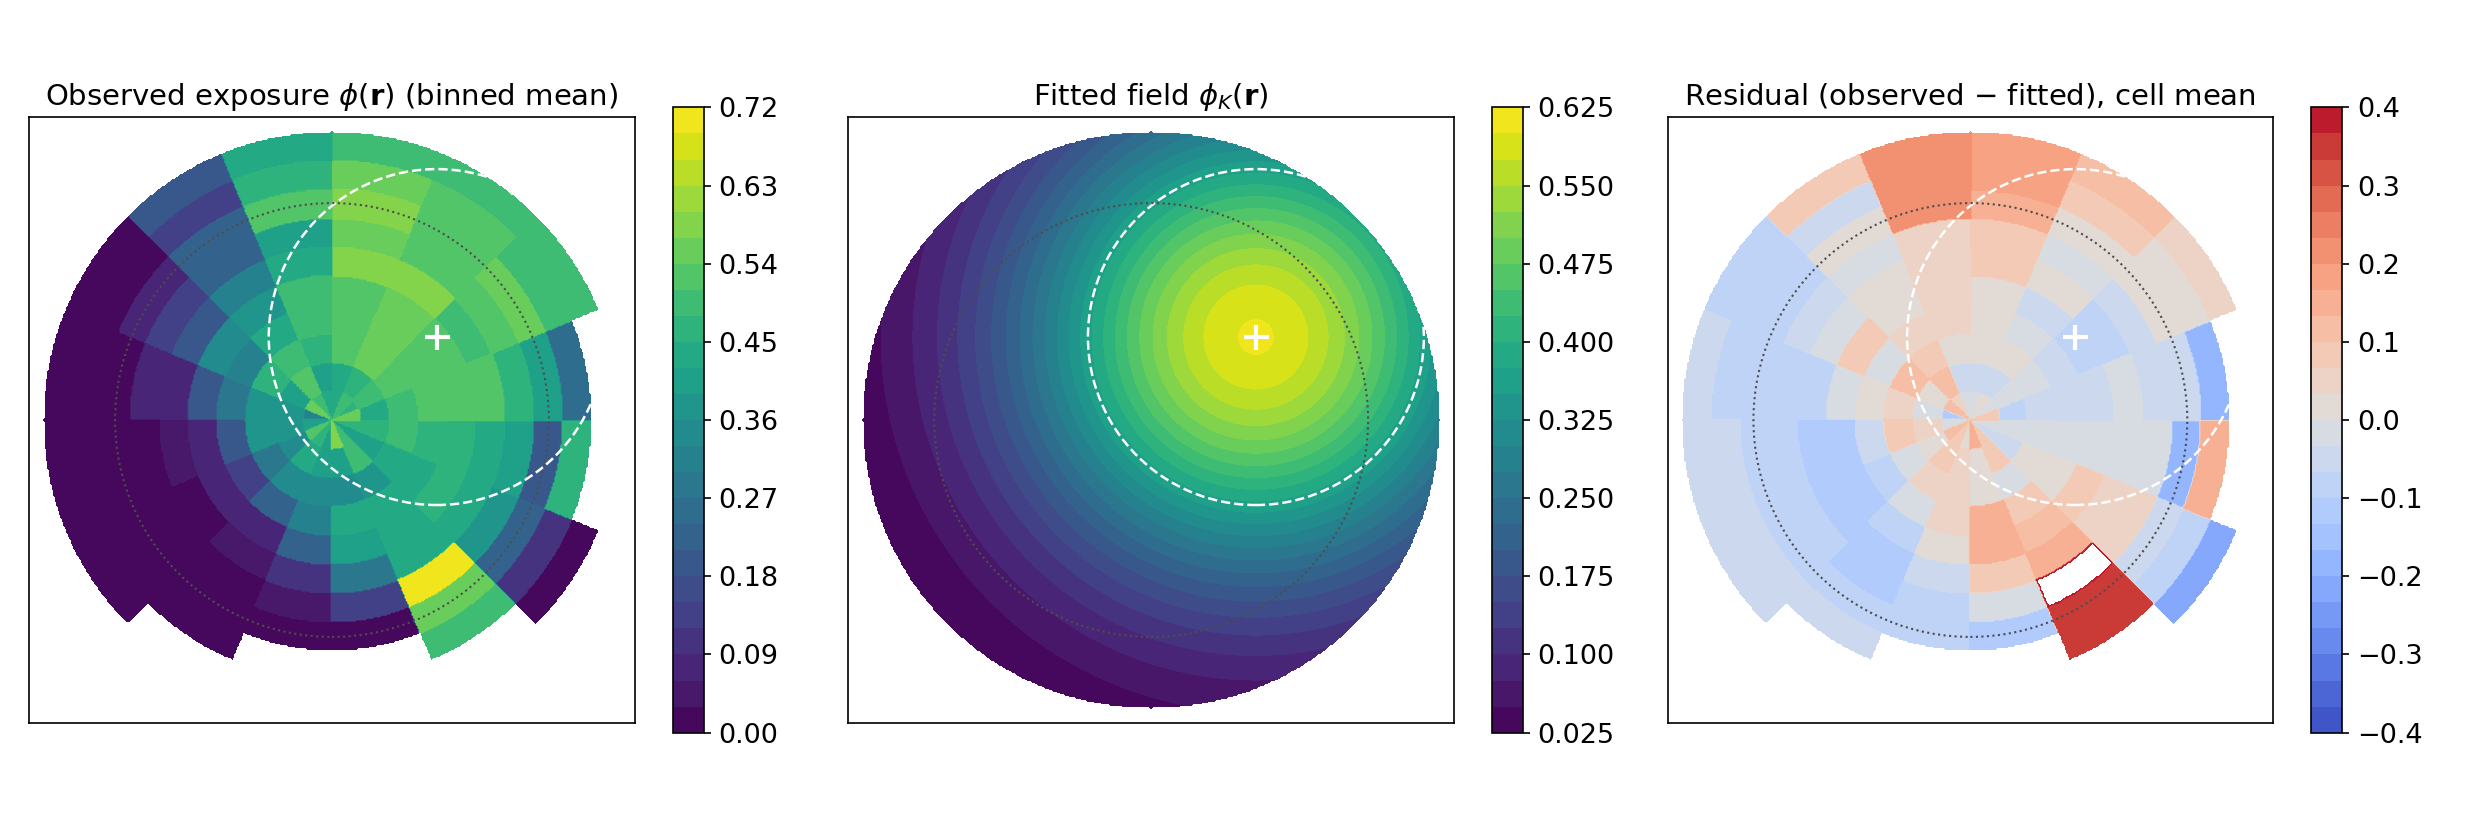
\includegraphics[width=\textwidth]{exposure_field_fit.png}
\caption{Task-level AI exposure surface and fitted cognitive technology
field.}
\label{fig:exposure-fit-new}
\end{figure}

The scale is a rule, and here the cognitive field
has nothing the robot field had. No aggregate displacement moment exists
for a technology still diffusing, so the rental $R$ is set instead so
that the gate binds in the calibrated field's core: capital cost
$R/(s_K\phi_K)\approx30$ at the centre against $\Pi\approx47$. The rule
is circular by construction and we state it as such. The level of the
automation cut is not identified, and the sweeps below report how far it
moves with the gate. The structure of the result does not move with it.

\begin{table}[!htbp]
\centering
\caption{Technology calibration. The cognitive field is fitted to task-level AI exposure by least squares. Fit is the $R^2$ on the smoothable between-cell exposure surface. The industrial-robot field, the second technology carried through the analysis, takes its centre, reach, and amplitude from Section~\ref{sec:robot-field}.}
\label{tab:technology-calibration-new}
\begin{tabular}{lcccccc}
\toprule
Field & $\xi_K$ & $\chi_K$ & $z_K$ & $A_K$ & Identification & Fit \\
\midrule
Cognitive & $38.4^\circ$ & $0.463$ & $0.583$ & $0.603$ & calibrated & $0.82$ \\
\bottomrule
\end{tabular}
\end{table}


\subsection{Displacement and the labour share}
\label{sec:cognitive-case}


The cognitive field operates the disk according to the price gate. Within
bands of equal technical effectiveness, the operated share orders
locations by price (the within-band rank correlation $\rho(a,\Pi)=0.99$ is a mechanical property of the takeover rule, not independent evidence).
Capital therefore moves first against dear work
within the exposed region (Figure~\ref{fig:operated-new}).

\begin{figure}[!htbp]
\centering
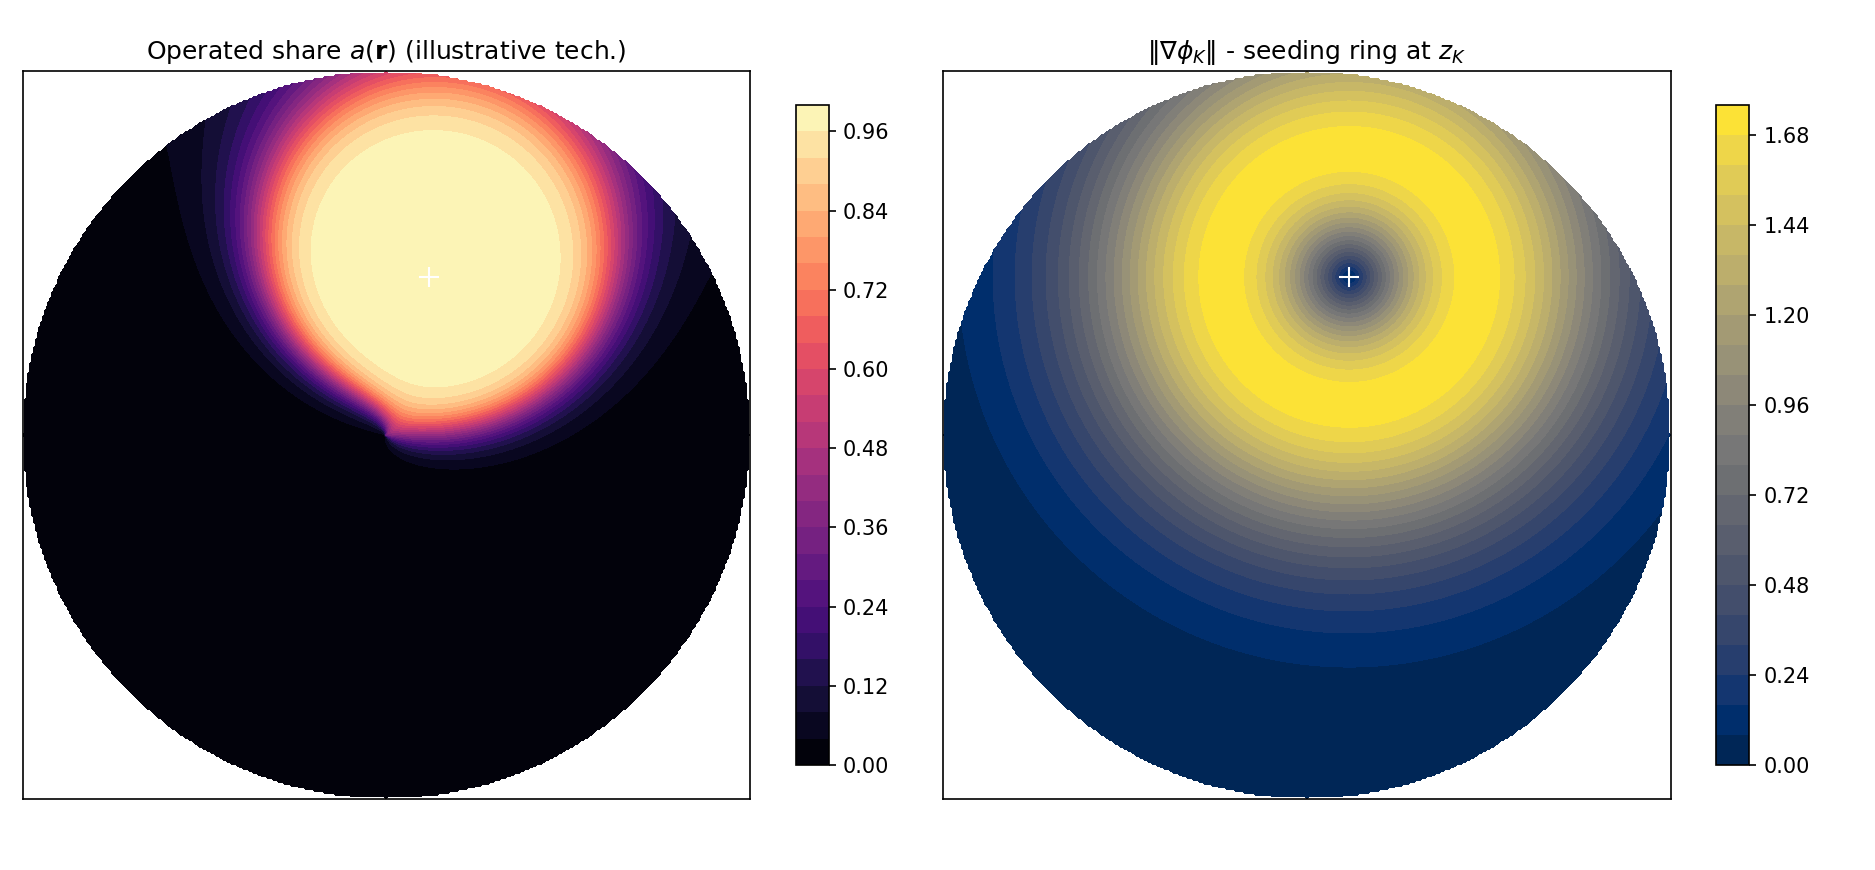
\includegraphics[width=\textwidth]{operated_share_demo.png}
\caption{Operated share and reinstatement boundary for the calibrated
cognitive field.}
\label{fig:operated-new}
\end{figure}

Solving the worker layer before and after bundle rewriting gives the
comparative static. The labour share falls substantially under pure
automation, from a pre-technology normalization of one to $0.649$,
and reinstatement does not restore it, leaving it at $0.644$ in the main
calibration. Task creation is not absent; much of the seeded mass
either fails to attach or attaches in lower priced regions. The
geometry withholds the aggregate recovery that a one-dimensional model
would assign to labour by construction. Aggregate employment does not
fall, because total labour is fixed and re-sorts; the comparison is
carried by pay and by who performs which work. The
result is robust to the family wage wedge: with the wedge in the
adoption gate, the share falls to $0.648$ under automation and $0.643$
after reinstatement, the unbound share of seeded mass is unchanged at
$68$ percent, and the ordering of gaining and losing occupations is
preserved. The wedge does move the volume of the re-sorting, which
rises from $13.7$ to $15.3$ percent of employment mass, because it opens
the gate wider on the well-paid families the field underprices.

The level of the automation drop is set by the gate. Sweeping $R$ from
$12$ to $24$ moves the post-automation share from $0.51$ to $0.78$,
because $R$ fixes how deep the technology cuts. The structure of the
result is not. Across a sixteenfold range of the attachment scale,
$\gamma$ from $0.25$ to $0.75$, both margin widths, and the attachment
shape, reinstatement moves the share by less than one percentage point
in either direction, against an automation drop of $22$ to $49$ points;
at the most generous corner it adds $0.4$ points. The unbound share of
seeded mass stays between $53$ and $79$ percent over the full sweep,
$61$ to $72$ within the attachment sweep. Re-sorted mass runs from $9$
to $19$ percent, set by the depth of the cut: cheap capital cuts deeper
and frees more labour. The claim the paper rests on is the gap between
task creation and wage recovery, not the level of the drop.

The shock relocates $14$ percent of employment mass. Losers are
exposed occupations whose high-priced bundle content is stripped:
clinical nurse specialists, sustainability specialists, software
developers. Gainers are the large low-priced service occupations that
absorb the freed labour: retail salespersons, baristas, fast-food
workers, cashiers. Binding also pulls employment toward occupations
able to perform the seeded tasks (the employment response correlates
with bound reinstatement at $+0.72$), but the absorption in levels
sits in low-barrier service work. The manual arc gains $0.04$ of
employment mass as displaced labour re-sorts there, without a
corresponding wage recovery because depth is weakly priced in that
direction.

\subsection{Who binds the new work}
\label{sec:cognitive-binding}

Of the seeded mass in the cognitive case, $27$ percent is captured by
capital, $5$ percent binds to existing occupations, and $68$ percent
survives capital but finds no bearer under the deficit gate. Of the
seed that survives as human work, $93$ percent is unbound. Its spatial
distribution marks the gap between task creation and occupational
absorption (Figure~\ref{fig:candidate-new}).

\begin{figure}[!htbp]
\centering
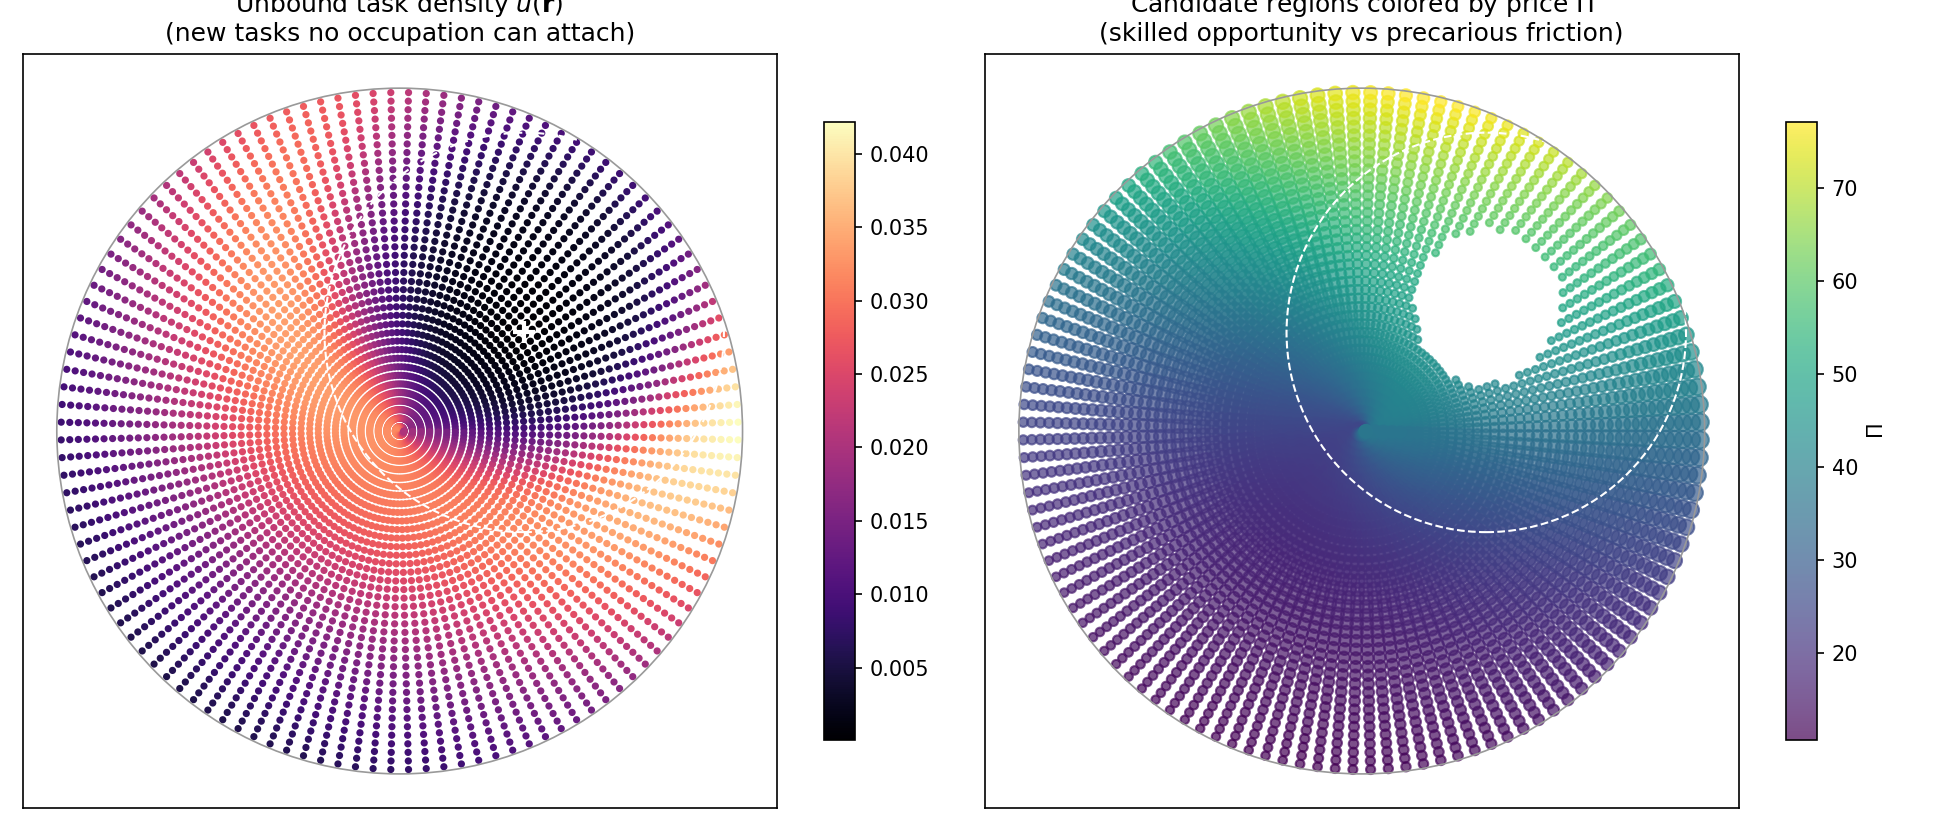
\includegraphics[width=\textwidth]{candidate_map.png}
\caption{Unbound task density and candidate regions for occupational
emergence.}
\label{fig:candidate-new}
\end{figure}

The reading follows Section~\ref{sec:unbound}: whether this mass is
latent skilled work or low-paid friction depends on the price at its
location. The model does not create new occupations; it identifies
where they may become necessary.

As under the robot field, the model does not name
the occupations that bind the remainder. Bound mass is dominated by
occupation size, because attachment capacity is capability weighted by
employment, and the ranking is headed by retail salespersons, baristas
and cashiers, the same occupations that head it under a field centred in
the opposite half of the disk. Bound mass per worker is flat across the
top of the ranking, a spread of $1.03$ over the top ten.

What the unbound mass is worth can be said, and it answers the question
Section~\ref{sec:unbound} leaves open. The unbound seed sits at $1.07$
times the mean price of work in the economy, above it, against the robot
field's $0.93$. This is not low-paid friction at the bottom of the
distribution. It is work the field creates that is priced above what the
economy pays on average and that no existing occupation reaches, and it
is $68$~percent of what the field seeds.

\subsection{Where the wage burden falls}
\label{sec:cognitive-wages}

The re-sorting that absorbs the freed labour has a wage consequence of
its own, and the analysis is incomplete without it. Existing
occupations take in the displaced mass by growing, and because local
capacity is congested ($\beta<1$), growth lowers the marginal return in
the receiving occupations. Each occupation's wage change decomposes
exactly into three channels: the content stripped from its bundle, the
congestion induced by inflow, and the new work it binds. Stripping
carries the mean, at an employment-weighted $-0.35$ log points, against
a congestion mean near zero ($-0.03$) and a reinstatement mean of
$+0.05$; the total is $-0.32$. Congestion is a distributional channel.
It moves a mean absolute
$0.10$ log points across occupations, twenty-nine percent of
stripping's magnitude, with the sorting signature: occupations that
gain employment crowd themselves ($-0.06$ on average), and the
thinned-out exposed occupations recover part of their loss ($+0.22$).
The split between the two channels is not order-invariant. Attributing
congestion before stripping rather than after moves the channel
magnitudes by $54$ percent, against a pre-registered tolerance of $25$
percent, so the decomposition ranks the channels and does not measure
either one precisely. The level is a full-maturity re-pricing rather
than a forecast.
Figure~\ref{fig:wage-deformation} maps the channel. The cognitive
field sits in the north, the freed labour re-sorts toward the
least-damaged parts of the structure, which are largely manual and
production directions, and the effective wage field is bent down where
it lands. The model predicts that cognitive automation transmits a
modest wage pressure into the production and manual occupations that
absorb the freed labour, through re-sorting rather than through the
technology's reach. This
prediction is directional; the cross-section of
Section~\ref{sec:directional-check} cannot identify it, and the
channel is consistent with the paper's other occupation wage
objects.\footnote{The stripping-only bundle wage change, the
first-order directional pressure of
Section~\ref{sec:directional-check}, and the congestion-inclusive value
change agree in sign against observed wage growth and rank occupations
consistently (Spearman $+0.84$ between the two stripping measures and
$+0.91$ once congestion is added, the congestion channel being small);
adding congestion does not move the
correlation with the confounded 2019--2025 cross-section, as it should
not.}

\begin{figure}[!htbp]
\centering
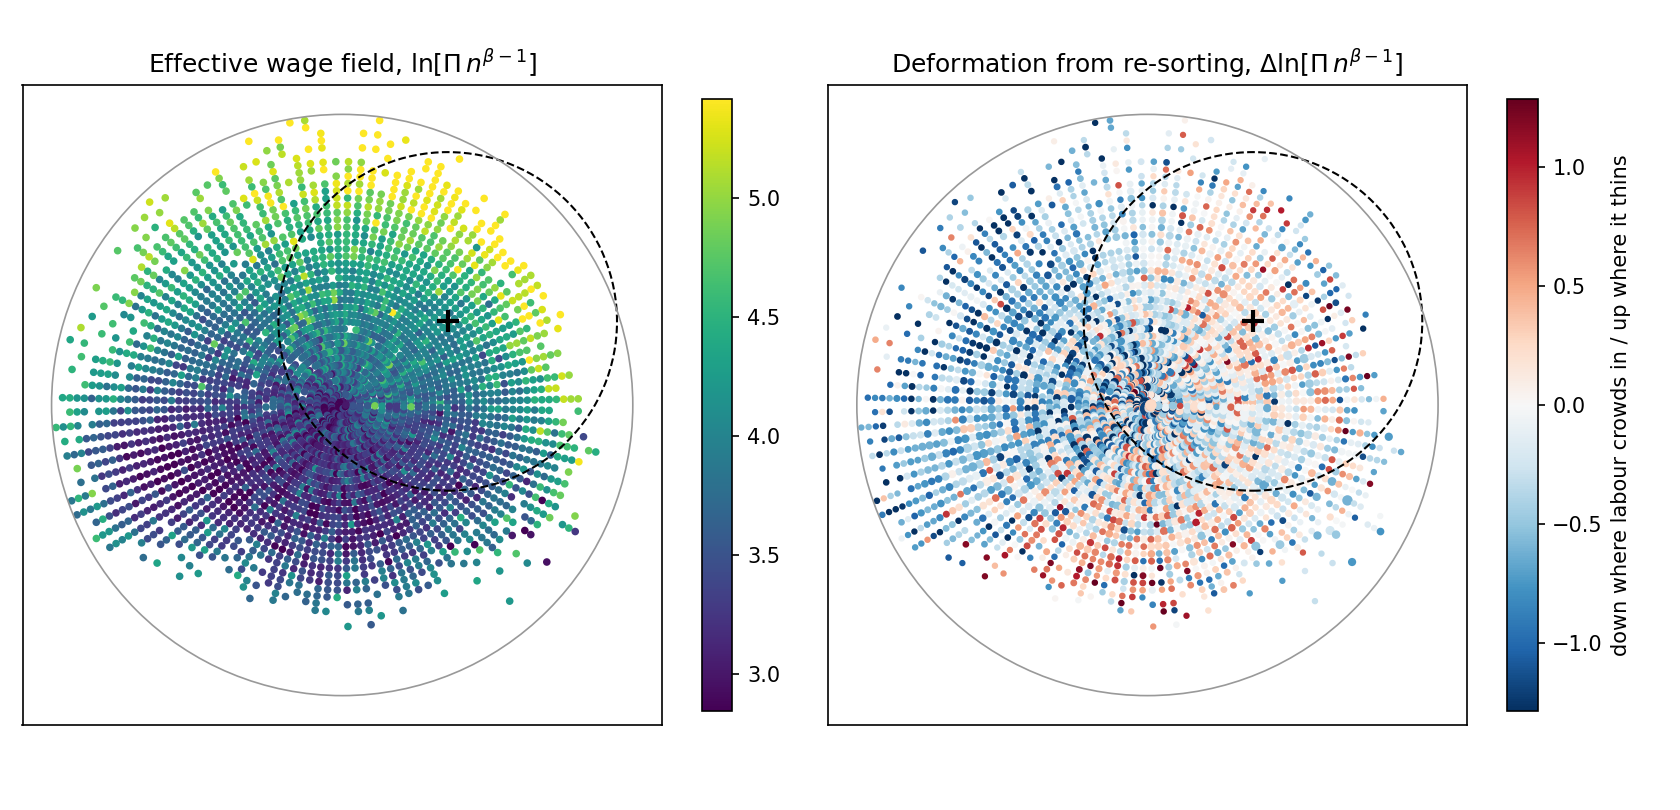
\includegraphics[width=\textwidth]{wage_field_deformation.png}
\caption{The effective wage field $\Pi(\mathbf{r})\,n(\mathbf{r})^{\beta-1}$
after re-sorting (left) and the wage pressure re-sorting induces (right),
over the task disk. Freed cognitive labour re-sorts toward the
least-damaged directions, largely the production and manual arc, where
crowding bends the effective wage down (blue). The technology field is
centred in the socio-cognitive north (cross); the burden falls on
occupations it does not reach.}
\label{fig:wage-deformation}
\end{figure}

The robot field locates the burden's source, and it
is not the new work. Within an occupation, capital takes content dearer
than that occupation's own average, at a ratio of $1.39$ against the
robot field's $1.17$: the price gate, mechanical in both. The difference
is where the fields are aimed. The content the cognitive field takes is
priced at $1.57$ times the mean price of work in its economy, against
the robot field's $0.83$, while the bound work it seeds lands at $0.92$
times that mean against the robot field's $0.89$. Bound new work lands
at nearly the same relative price under both technologies. What differs
is what was taken. The cognitive wave trades work priced well above the
average for work priced slightly below it, an exchange of $0.59$ to one,
and $0.53$ when the seeded work is priced at the centroid of the
occupation that binds it. Reinstatement returns $15$~percent of the wage
value stripping removes, against $121$~percent under the robot field.
Automation costs wages when it destroys work dearer than the work it
creates, and in this model the geometry decides which.

\subsection{Against the data}
\label{sec:cognitive-data}
\label{sec:directional-check}
\label{sec:check-confound}

The cognitive wave's own wage window is 2019 to 2025, and it cannot test
the model. We show that at length, because the way it fails is a caution
that reaches past this paper: the model's wage prediction and the
dominant wage shock of the period load on the same index, and an
occupational cross-section cannot tell them apart. The robot wave's
window, in Section~\ref{sec:robot-data}, does not have that problem.

The wage claim is directional. If automation and
reinstatement push an occupation's bundle down the price gradient, that
occupation should experience weaker wage growth than occupations whose
bundles move less or remain closer to high-priced work. We confront that
implication with observed occupational wage changes in two steps, a
naive directional check, which the model passes, and a confound
analysis, which shows the pass is uninformative in this window. The
second step matters beyond this paper.

Using the calibrated cognitive field, each occupation's bundle is
rewritten and its centroid shifts from $\mu_o$ to $\mu_o^{\text{post}}$. The
predicted directional wage pressure is
\begin{equation}
  \widehat{\Delta\ln\Pi}_o
  =
  \Delta\mu_o\cdot\nabla\ln\Pi(\mu_o).
  \label{eq:directional-pressure}
\end{equation}
A negative value means that the bundle moves down the price gradient.
Because the prediction is negative for almost every occupation, a
\emph{positive} rank correlation with wage growth means that occupations
with more severe down-gradient shifts see lower wage growth.

We compare this predicted pressure to observed OEWS median hourly wage
changes between May 2019 and May 2025 (the latest OEWS release), matched
by SOC code; $725$ of $849$ occupations ($640$ distinct SOC codes) carry
a median wage in both vintages. Because the match is many-to-one and the
wages nominal, we compare ranks, which differences out the common
nominal drift (mean $\Delta\ln w\approx+0.22$). The field pushes almost
every bundle down-gradient ($96$ percent), and the naive check passes:
the rank correlation between predicted pressure and observed wage change
is $+0.34$ across occupations ($p<10^{-20}$) and $+0.35$ at the SOC
level; the model's own bundle wage change tracks observed changes
slightly better ($+0.42$), and the result is stable when May 2024 is
used as the endpoint ($+0.39$).

This looks like support for the mechanism. It is not. The predicted pressure is nearly collinear with the
baseline wage level: because the price gate targets dear work,
occupations with high 2019 wages are pushed furthest down-gradient (rank
correlation $-0.57$ between predicted pressure and baseline wage). And
the window contains the pandemic-era compression of the US wage
distribution, in which low-wage occupations saw exceptional relative
wage growth for reasons unrelated to automation
\parencite{autor2023compression}: baseline wage alone predicts wage
growth at rank correlation $-0.58$. The model and the compression
therefore make the same cross-sectional prediction, and the raw
correlation cannot distinguish between them.

The data resolve the collinearity in favour of the confound. Controlling
for the baseline-wage rank, the partial rank correlation between
predicted pressure and wage growth is $+0.02$ ($p=0.57$); the bundle
wage change performs no better ($+0.03$). Adding the mechanism raises
the rank-$R^2$ already achieved by baseline wage alone by $0.0003$. The
fine structure points the same way: the wage-growth gradient is
steepest where the field barely reaches and nearly flat where it is
strongest, and among above-median-wage occupations, where the mechanism
strips the most and the compression matters least, the raw correlation
vanishes entirely ($-0.03$). This is compression at the bottom of the
distribution, not high-priced content stripped in the exposed
region.

A window split settles the matter. The OEWS 2023 vintage divides the
period into 2019--2023, which contains the peak of the compression and
essentially predates the deployment of the technology the field is
calibrated to, and 2023--2025, the period of actual diffusion.
Table~\ref{tab:window-split} and Figure~\ref{fig:centroid-shift-new}
report the result: the entire raw
correlation lives in the pre-deployment window, and in the deployment
window it is absent, along with most of the compression gradient itself.

A placebo makes the machinery explicit. We repeat the exercise with two
technologies that make no claim about the period's wage changes: the
industrial-robot field of Section~\ref{sec:robot-field}, a real
technology whose deployment predates the window
\parencite{acemoglu2020robots}, and a rotated clone of the cognitive
field, a technology that does not exist. The robot field returns the
null. Its predicted pressure loads only weakly on the wage level
(collinearity $-0.09$ against the cognitive field's $-0.57$), so the
compression hands it nothing: the raw correlation is $+0.04$ ($p=0.25$),
gone under conditioning and absent in every window
(Table~\ref{tab:window-split}). The rotated clone, sitting mostly in
cheap territory where the gate barely opens, loads on the wage level at
$+0.22$ and collects a weak but significant correlation ($-0.13$,
$p=4\times10^{-4}$), null given baseline wage and confined to
2019--2023. The two placebos bracket the mechanism. What the naive check
finds is set by how strongly a footprint loads on the wage level, not by
the technology's relevance to the period. A real technology whose wave
is over returns the null. A nonexistent one that loads on the wage level
still clears conventional significance. The cognitive field, loading
hardest, is the $+0.34$ that vanishes under conditioning.

\begin{table}[!htbp]
\centering
\caption{Window split of the directional check. Spearman rank
correlations between predicted directional wage pressure and observed
wage change; the partial correlation controls for the rank of the wage
level at the start of each window. The baseline gradient is the rank
correlation between the starting wage level and wage growth ($N=725$).
The placebo panel repeats the exercise with the industrial-robot field
of Section~\ref{sec:robot-field}, a technology whose deployment
predates the window; its pressure loads only weakly on the wage level,
so its raw correlation is near zero.}
\label{tab:window-split}
\begin{tabular}{lccc}
\toprule
Window & Raw & Partial $\mid$ baseline wage & Baseline gradient \\
\midrule
\multicolumn{4}{l}{\emph{Calibrated cognitive field}} \\
2019--2023 (pre-deployment) & $+0.34$ & $+0.03$ & $-0.56$ \\
2023--2025 (deployment) & $+0.04$ & $-0.03$ & $-0.11$ \\
2019--2025 (full) & $+0.34$ & $+0.02$ & $-0.58$ \\
\midrule
\multicolumn{4}{l}{\emph{Placebo: robot field}} \\
2019--2023 & $+0.03$ & $-0.02$ & $-0.56$ \\
2023--2025 & $+0.03$ & $+0.02$ & $-0.11$ \\
2019--2025 & $+0.04$ & $-0.01$ & $-0.58$ \\
\bottomrule
\end{tabular}
\end{table}

\begin{figure}[!htbp]
\centering
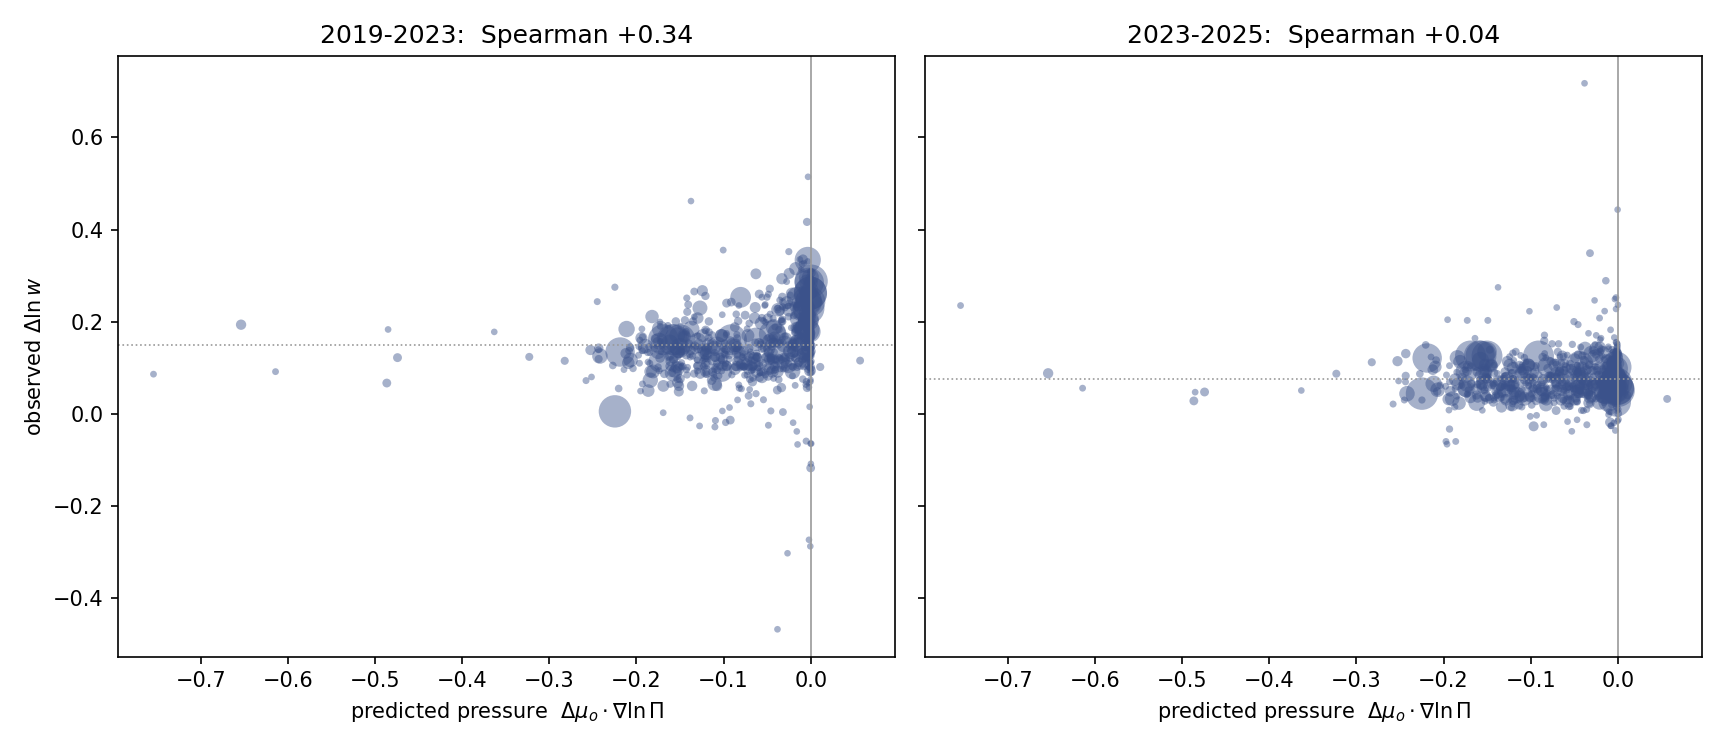
\includegraphics[width=\textwidth]{centroid_shift_test.png}
\caption{Predicted directional wage pressure against observed
occupational wage change, split at the OEWS 2023 vintage. The raw
correlation is confined to the 2019--2023 window, which contains the
peak of the pandemic wage compression and predates the deployment of the
technology the cognitive field is calibrated to; in the 2023--2025
window it is absent.}
\label{fig:centroid-shift-new}
\end{figure}

This window therefore fails to contradict the model because it cannot
discriminate, which is not the same as support, and we do not present it
as such. The window that can discriminate is the robot wave's
(Section~\ref{sec:robot-data}), where the pressure measure is orthogonal
to the wage level, the correlation survives conditioning on the wage
level and on the manufacturing share, and the counterfactual fields carry
the opposite sign. What that window cannot do is attribute, since robots
and import competition pressed the same occupations. The firm locations
of Section~\ref{sec:check-newwork} are different again, bearing on a
spatial prediction no wage series can make. None of the three readings is
proof. A cross-section of firm positions cannot separate seeding at the
boundary from other processes that would deposit new work there, and an
occupational wage window cannot separate contemporaneous pressures on the
same arc.

The wage mechanism still has a proper test, and the cross-section is not
it. The identifying variation the model calls for is within-occupation
task recomposition over time, whether the paid content of exposed
bundles is redrawn in the direction the operator predicts. That test
needs within-occupation microdata of the kind pioneered by
\textcite{atalay2020evolution}, and we leave it to future empirical
work. The null in the deployment window is not evidence against the
model either. The model does not predict that two years of diffusion
should be visible in occupational median wages, and a strong pass there
would itself have been suspect.

The exercise carries a wider caution. A naive correlation between AI
exposure and 2019--2025 occupational wage growth has the right sign, a
small $p$-value, and nothing to do with AI. It measures the pandemic
compression. This is the exposure-versus-incidence distinction of
Section~\ref{sec:operated-share} in empirical form. Technical exposure
correlates with wage levels, wage levels drove relative wage growth in
this period, and the chain of correlations manufactures apparent support
for any mechanism whose cross-sectional footprint is a wage gradient,
strongest where that footprint is steepest. Work relating occupational
AI exposure to wages in this period \parencite{hampole2025} contends
with the same collinearity, and a design resting on the occupational
cross-section alone cannot break it.

The two fields can now be set side by side. Table~\ref{tab:two-fields}
does that, and the levels in it are not the comparison: the robot shock is
the size the robot era delivered, the cognitive shock is the size the
rental rule implies, and the two columns are not on one scale. The rows
below the labour share are ratios inside each economy, and those are.

\begin{table}[!htbp]
\centering
\caption{The two fields. Each runs through the same model in its own
era, with its own price field and employment weights. The robot shock
takes its scale from an external displacement moment and the cognitive
shock from the rental rule, so the levels are not comparable across the
columns; the structure is. Prices are divided by the mean price of work
in each field's own economy.}
\label{tab:two-fields}
\begin{tabular}{lcc}
\toprule
 & Industrial robots & Cognitive \\
\midrule
Scale from & displacement moment & rental rule \\
Labour share, automation & $0.9948$ & $0.6488$ \\
Labour share, reinstatement & $0.9925$ & $0.6439$ \\
Reinstatement gap & $0.23$ pts & $0.49$ pts \\
Unbound share of seeded mass & $93\%$ & $68\%$ \\
\midrule
Price of the content capital takes & $0.83\times$ & $1.57\times$ \\
Price where bound new work lands & $0.89\times$ & $0.92\times$ \\
Exchange rate, lands over takes & $1.07$ & $0.59$ \\
Price of the unbound mass & $0.93\times$ & $1.07\times$ \\
Reinstatement over stripping & $121\%$ & $15\%$ \\
\bottomrule
\end{tabular}
\end{table}

Reinstatement fails to restore the labour share under both technologies,
and the gap is under half a point in each. The unbound share is large in
each, and in each it is invariant to the scale of the shock. Neither is
a property of where the cognitive field happens to sit. What position
governs is the price of the work each wave destroys, which is the last
three rows of the table.

%% ============================================================
\section{Where new firms appear}
\label{sec:check-newwork}

The calibration can be confronted with firm locations it never used.
Reinstatement seeds new tasks where the technology field changes most
rapidly, on the ring at radius $z_K$ where $\|\nabla\phi_K\|$ peaks
\eqref{eq:gradient-phi}. This is the two-dimensional form of an
older claim. In the one-dimensional model, new tasks enter at the top of
the task index, above the range capital has taken, where labour holds
the comparative advantage
\parencite{acemoglu2018race,acemoglu2019automation}. The field lifts
that top to a boundary. New work should appear at the boundary, away
from the technology centre. A ranking of occupations by automatability
\parencite{frey2017, felten2021occupational} has no boundary and no
gradient, so it cannot place new work at all.

The validation needs firm locations fixed without reference to where
the model seeds. We take the AI and robotics startups of
\textcite{fenoaltea2026}, tagged from the Y~Combinator directory
($n=1894$ and $155$; $78$ carry both tags). Each firm's product text is
embedded with the encoder of \textcite{storck2026geometry} and mapped
through the frozen projection, which was calibrated to O*NET task
statements and to wages and never to where firms are founded. A control
corpus of $1{,}500$ companies from the same directory carrying neither
tag, embedded and projected identically, supplies the empirical null:
whatever placement generic startup text receives, the technology groups
must exceed it. Document embeddings shrink norms toward the corpus
mean, so radial positions are conservative; angular placement carries
the group separation and is unaffected.

The two populations take distinct positions, and the ring lies between
them (Figure~\ref{fig:startup-comparison}). The AI firms sit on the
ring's inner flank: median distance $0.45$ to the technology centre
against the control's $0.49$, with disjoint bootstrap intervals, a
compass shifted toward the analytical north, and incidence-field
density $0.92\times$ the disk mean against the control's $0.30\times$,
three times more capability-near than generic startup text, on the side
of the boundary where the model binds new work to existing occupations.
The robotics firms sit on the outer western arc: $65$ percent in the
technical-physical west against the control's $11$, out of the
incidence core entirely ($0.03\times$), under the arc the model keeps
unbound. Raw radial statistics do not carry the comparison: any
document corpus shrinks toward the centre of the projected cloud, which
itself sits near the ring radius, so the control matches the disk-null
ring enrichment ($1.33\times$ against the technology groups' $1.30$
and $1.34$) and the discrimination runs on structure. A cross-section
of this kind cannot confirm the prediction; it could have contradicted
it, with populations in the core or where the control sits, and does
not.

Bound reinstatement does not spread evenly around the ring. It
concentrates in two lobes, one near the technology centre and one in the
technical-physical west, which appear as two peaks in the radial profile
of $B_o$ (Figure~\ref{fig:startup-comparison}). The two technologies
fill a lobe each, and the split follows from where each sits in the
geometry rather than from a second mechanism. AI firms sit on the inner
lobe, where existing occupations can bind the new work. Robotics firms
sit on the outer lobe, off the incidence core entirely, where the
seeded work binds to no existing occupation. A scalar exposure ranking
scores the two alike. Pooled, the firms trace both peaks of the model's
bound reinstatement.

\begin{figure}[!htbp]
\centering
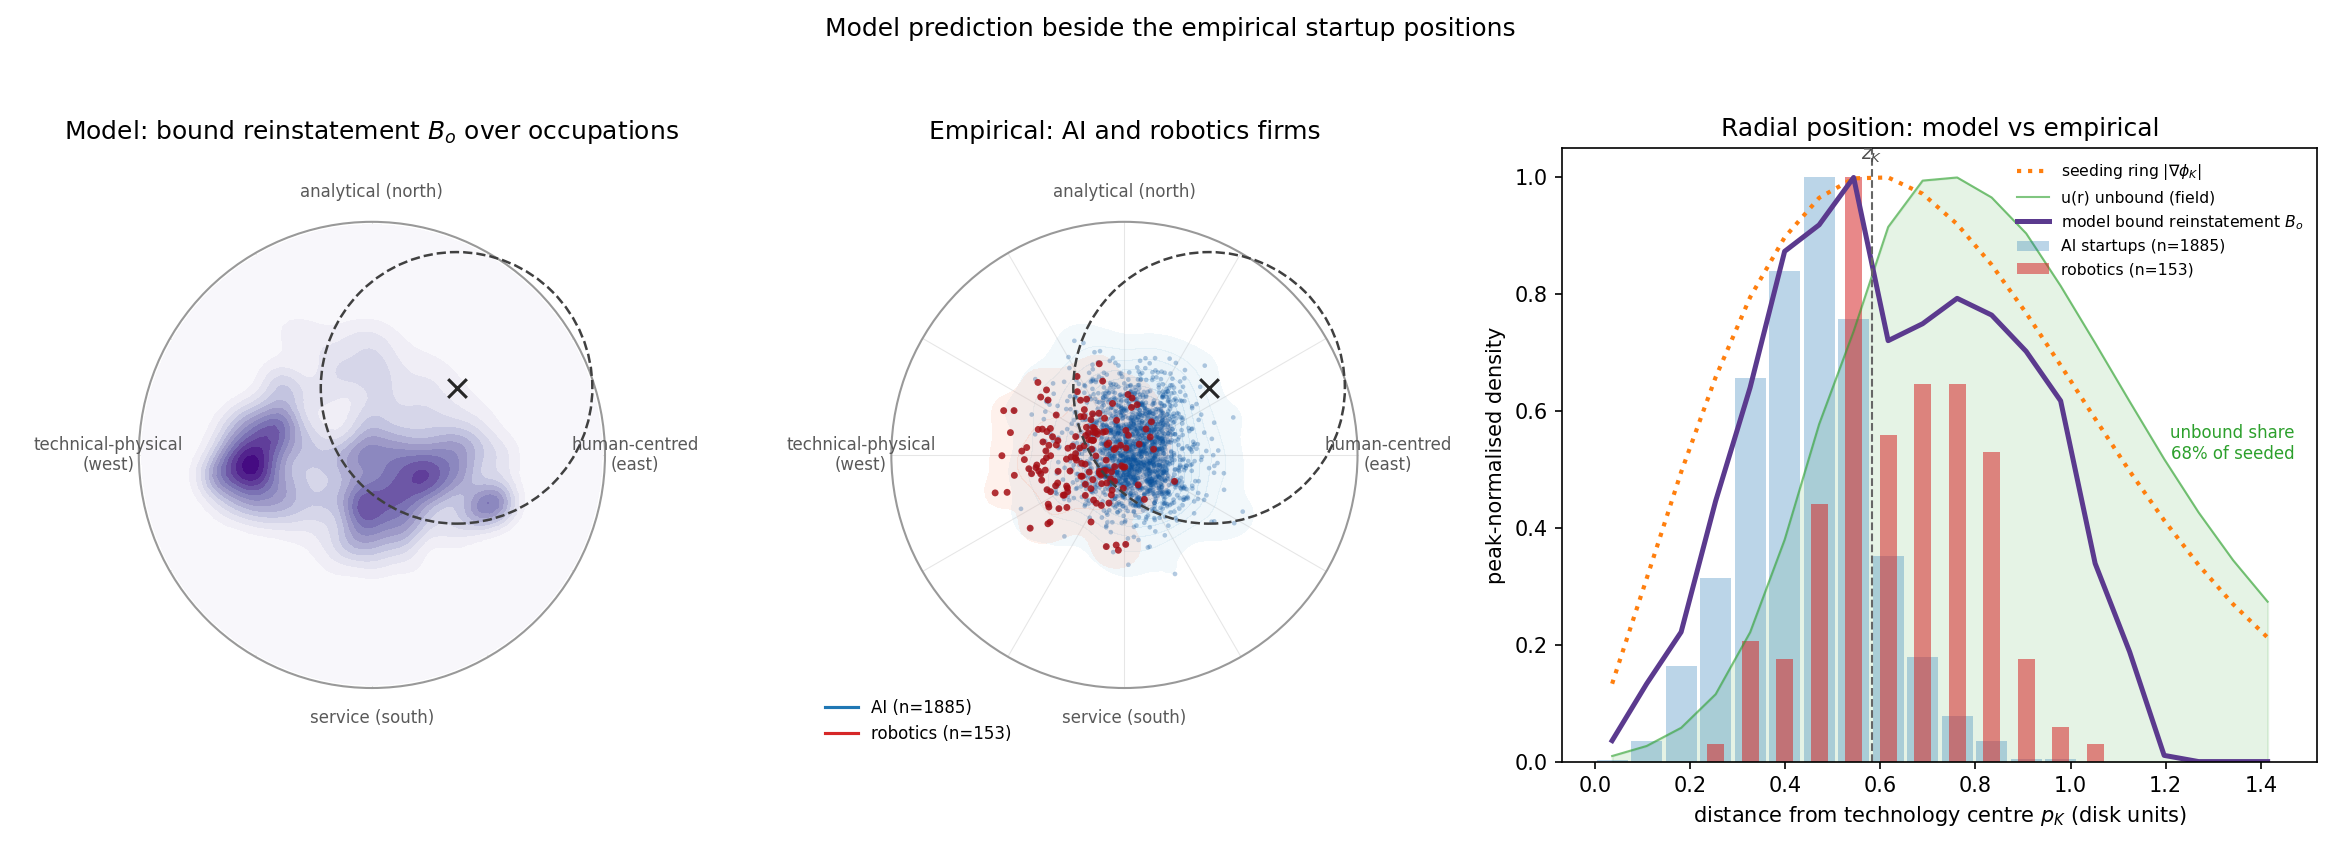
\includegraphics[width=\textwidth]{startup_field_enrichment_comparison.png}
\caption{The model's prediction beside the firm positions, on the same
disk. Left: bound reinstatement $B_o$ over occupations, concentrated on
the seeding ring at radius $z_K$ (dashed) around the technology centre
$p_K$. Middle: AI firms (blue) and robotics firms (red) from
\textcite{fenoaltea2026}, placed by their product text through the frozen
projection; grey points are the control corpus. Right: radial density
against distance from $p_K$; the seeding ring $\|\nabla\phi_K\|$, the
unbound field $u(\mathbf r)$, and the model's bound reinstatement peak
near $z_K$, and so do both firm groups. So does the control corpus, so
the radial peak is not the evidence; the groups separate on the flank
they occupy. The unbound share of seeded
mass is $68$ percent. The firm positions are calibrated to O*NET and
wages, never to where firms are founded.}
\label{fig:startup-comparison}
\end{figure}


%% ============================================================
\section{Discussion}
\label{sec:discuss}
%% ============================================================

The central contribution of the paper is to locate automation and
reinstatement in a priced task space. Reinstatement is not an aggregate
return of labour to production. It is a spatial process in which new
tasks must survive capital and then bind to existing capabilities. The
same amount of task creation can therefore have different consequences
depending on where it appears.

This yields a distributional result that one-dimensional models cannot
state. Reinstatement returns human task mass wherever it lands. It
returns pay only where the price field rewards the restored work. New
tasks in socio-cognitive directions can restore both work and pay. New
tasks in manual or service directions may restore work without
restoring pay.

Run through the model, the mechanism gives the paper's quantitative
answer, and it gives it twice. Under the cognitive field, automation cuts
the labour share from one to $0.649$, and reinstatement leaves it at
$0.644$, because $68$~percent of the seeded mass binds to no occupation.
Under the industrial-robot field, whose scale is fixed not by a rule but
by the aggregate displacement its own era delivered, the cut is small and
reinstatement again fails to close it, with $93$~percent of the seed
unbound. The reinstatement gap is under half a point in both, and in both
the unbound share is invariant to the scale of the shock. Neither is a
property of where the cognitive field happens to sit. Position governs
the price of the work a wave destroys, and it is there the two waves
part: the robot wave took work its economy paid below the average for,
and the cognitive wave takes work it pays well above the average for.

The model also clarifies the Turing-trap logic \parencite{brynjolfsson2022turing}. Default automation strips
high-priced task content from occupational bundles. Default
reinstatement often refills them with tasks that are easier to bind
because they demand no new priced capabilities. The occupation remains,
but its paid content declines.

The unbound tail is a watch region. Much of the seeded mass the model
keeps unbound lies under the outer western tail of the seeding ring,
where the robotics firms already sit and where no existing occupation
reaches. The model makes the forward question precise: if boundary
seeding is right, the coming years should deposit new firms and new
occupational tasks under that tail before existing occupations can
carry them. The startup cross-section is a first reading of a process
that has barely begun.

The model keeps exposure and incidence separate. Technical exposure is
what a technology can do; economic incidence is what it is paid to do.
A weak raw correlation between exposure and wages does not refute the
mechanism, because adoption depends on exposure relative to price. The
price field turns exposure into incidence.

Several limitations bound the results, and each is a stated primitive,
not an oversight. The comparative statics hold the readiness
fields $e_o$ fixed between the two rest points: capability acquisition
is treated as slower than the shock, a timescale separation in the
spirit of \textcite{adao2024fast}. The attachment capacity
$C(\mathbf{r})$ is linear in employment. Output demand is not modelled:
revenue at a location does not respond to the cost saving automation
produces, so the channel that can turn labour-saving technology into
employment growth is outside the analysis. The price field is held fixed
under
the technology shock, even though it can be interpreted as an
assignment-equilibrium object. Re-solving the assignment after the
shock is a first-order extension that should dampen displacement by
allowing the price of crowded or cheapened work to adjust; the present
paper deliberately holds $\Pi(\mathbf{r})$ fixed to isolate the spatial
automation and reinstatement mechanisms.

The model is also static: it compares two rest points, and unbound
tasks are read off as a density rather than accumulated as a stock.
The fate accounting suggests that this is the most promising
continuation of the framework. If unbound mass accumulates while
occupations absorb new work at a finite pace, the speed of the shock
relative to the speed of absorption becomes an economic variable in
its own right, and the destination of reinstated work --- which
occupations end up holding it --- may depend on the path and not only
on the endpoint. We regard a dynamic treatment built on these
observations as interesting future work. The firm positions make this
concrete. AI and robotics firms occupy the bindable part of the seeded
region, and the unbound field extends radially beyond them
(Figure~\ref{fig:startup-comparison}). One reading is that the outer
band holds seeded work not yet organised into occupations, latent room
for new firms and new kinds of work. A cross-section cannot tell that
apart from an outer band that stays sparse because its work resists
binding, which is the distinction a stock-based dynamic treatment would
draw.

The wage wedge also opens a connection to rent-based accounts of
automation \parencite{acemoglu2024rents}. If the residual wedge is interpreted as an occupation- or
family-level rent, the same price gate implies that high-wedge work is
more likely to cross the adoption margin. The within-group compression
implications of that extension require rent dispersion within exposed
groups and are left to separate work.

The main implication is simple. The question is not whether automation
creates new tasks. The question is where those tasks appear, whether
labour keeps them, and whether the workers who can bind them already
hold the priced capabilities they require.

%% ============================================================
\section*{Data and code availability}

All inputs, code, and frozen outputs are public at
\url{https://github.com/JoakimStorck/technology-fields}. Every
result-bearing number in the paper traces to a producing script in
\texttt{scripts/}, with its output frozen in \texttt{results/}; the
pre-registered placebo test records its hypotheses in the producing
script's docstring, as does the field-form invariance check reported in
Section~\ref{sec:technology-model}.

\printbibliography

%% ============================================================
\appendix

\section{The assignment programme}
\label{app:assignment}

This appendix specifies the assignment equilibrium that microfounds
the price field and reports the test sequence that selects it. All quantities are computed on the frozen
inputs of Section~\ref{sec:frozen-inputs}; no observed wage enters any
computation, so agreement with the estimated field of
eq.~\eqref{eq:price-estimates} is a test of the interpretation, not a
fit to its target.

The field is not a simple scarcity price. If tasks were priced by a CES
aggregator under uniform demand, price would fall with output density;
in the data it barely responds
($\partial\ln\Pi/\partial\ln n_0 = -0.03$, an implied substitution
elasticity of about $35$), and the dear socio-cognitive arc is the
densely staffed one. Nor are the capability coefficients ordinary
factor prices: they do not rise with capability scarcity, and one is
negative once the others are held fixed, so they read as hedonic
coefficients rather than prices of factors in fixed supply. Log price
is, however, almost exactly linear in priced capability content
($R^2 = 0.96$). The field is therefore better read as an assignment
price in the sense of multidimensional sorting \parencite{lindenlaub2017}:
the shadow price of matching heterogeneous capability bundles
to heterogeneous task requirements under directionally biased demand.

The numerical assignment closure makes this concrete. Occupations are
capability types whose productivity at a task location is their
readiness in priced capabilities, the same object that later governs
task attachment (Section~\ref{sec:deficit-gate}); task demand is CES
over locations, and each occupation allocates its employment toward
locations that pay well relative to its readiness. No observed wage
enters the computation, so agreement with the estimated field is a
test rather than a fit. The comparison statistic is the directed
gradient: the difference in median $\ln\Pi$ between a deep
socio-cognitive reference arc and a deep technical--service reference
arc (below); the estimated field puts it at
$+0.39$. With uniform demand, the assignment recovers the shape of the
reduced-form field (rank correlation $+0.92$) but produces a directed
gradient of only $+0.08$. A single cognitive demand shifter,
\[
  \alpha(\mathbf{r})
  =
  \exp(\lambda q_{S1}(\mathbf{r})),
\]
steepens the gradient to $+0.36$ while preserving the shape (rank
correlation $+0.97$ at $\lambda=0.2$;
Figure~\ref{fig:price-microfoundation}). A
production-complementarity alternative concentrates labour in the north
but makes it too cheap, because output expands faster than price: the
correlation between wages and the price surface turns negative. The
dearness of cognitive work is therefore better understood as
demand-driven assignment pressure than as productivity superiority.

The implication for this paper is limited but important. The price field
can be treated as an equilibrium object: a capability-assignment cost
surface with a demand-driven cognitive premium. The comparative statics
below hold that surface fixed. Re-solving the assignment after a
technology shock is a general-equilibrium extension and is expected to
dampen, not reverse, the mechanisms studied here.

\begin{figure}[!htbp]
\centering
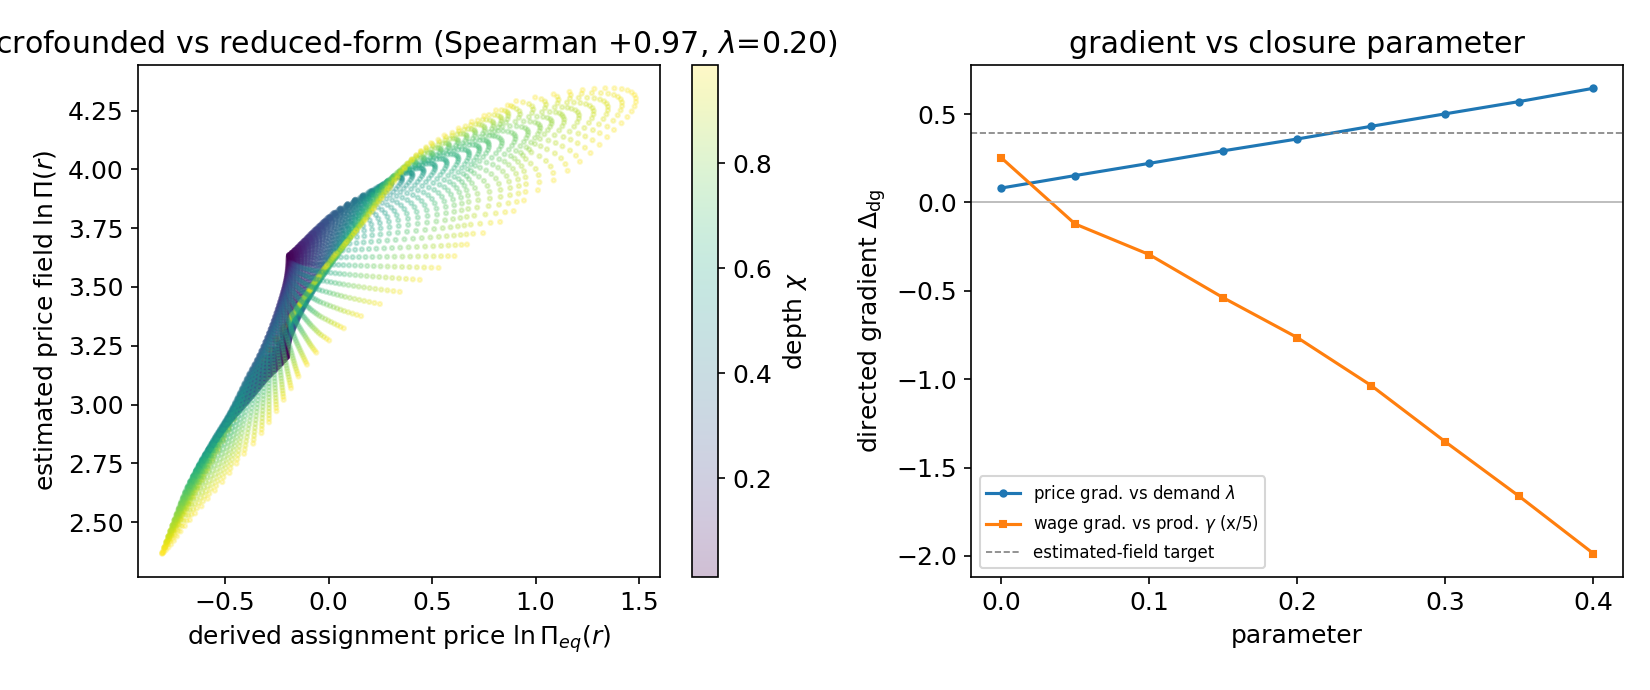
\includegraphics[width=\textwidth]{price_microfoundation.png}
\caption{Assignment interpretation of the price field. The calibrated
assignment price reproduces the reduced-form field closely when demand
is biased toward cognitively intensive tasks.}
\label{fig:price-microfoundation}
\end{figure}

\subsection*{The programme}

Task locations are the cells of a polar grid over the disk, with
baseline task-work density $n_0(\mathbf{r})$ built from occupational
bundles and employment. Occupations are capability types. The
productivity of occupation $o$ at location $\mathbf{r}$ is its
readiness $e_o(\mathbf{r})$ of eq.~\eqref{eq:attachment}, evaluated at
the calibrated acquisition scale: the same primitive that governs task
attachment in the main model governs comparative advantage here.

Demand for task output is CES over locations with substitution
elasticity $\sigma = 3$ and location weights $\alpha(\mathbf{r})$,
uniform in the baseline. With aggregate output
$\bar Y = \bigl(\sum_{\mathbf{r}} \alpha\, y^{\rho}\bigr)^{1/\rho}$,
$\rho = (\sigma-1)/\sigma$, the inverse demand at a location is
\[
  \Pi_{\mathrm{eq}}(\mathbf{r})
  =
  \alpha(\mathbf{r})
  \left(
    \frac{\bar Y}{y(\mathbf{r})}
  \right)^{1/\sigma},
\]
normalized to mean one as numeraire. Each occupation allocates its
employment over locations by a logit in the payoff
$\Pi_{\mathrm{eq}}(\mathbf{r})\,e_o(\mathbf{r})$ with smoothness
$\kappa$, set to half the mean price. Output at a location is the
readiness-weighted employment allocated there,
$y(\mathbf{r}) = \sum_o L_o\, s_o(\mathbf{r})\, e_o(\mathbf{r})$, and
the fixed point of prices and allocations is found by damped
iteration. Occupation earnings per worker are
$w_o = \sum_{\mathbf{r}} s_o(\mathbf{r})\,
\Pi_{\mathrm{eq}}(\mathbf{r})\, e_o(\mathbf{r})$.

The comparison statistic used throughout is the directed gradient
$\Delta_{\mathrm{dg}}$: the difference in median $\ln\Pi$ between a
deep socio-cognitive reference arc ($\cos\xi > 0.5$, $\chi > 0.4$) and
a deep technical--service reference arc ($\cos\xi < -0.3$,
$\chi > 0.3$). On the estimated field of
eq.~\eqref{eq:price-estimates} the directed gradient is $+0.39$; on
log employment density it is $+0.71$, so the dear side of the disk is
also the densely staffed side.

\subsection*{The test sequence}

\emph{T1, task scarcity: rejected.} If the field were a CES scarcity
price under uniform demand, $\ln\Pi$ would fall in log density with
slope $-1/\sigma$. The estimated slope is
$\partial\ln\Pi/\partial\ln n_0 = -0.028$ (rank correlation $-0.12$),
an implied elasticity of about $35$, and the directed density gradient
of $+0.71$ puts the mass where the price is high. Scarcity does not
generate the field.

\emph{T2, capability pricing: confirmed.} Log price is nearly linear
in priced capability content:
$\ln\Pi \sim a + b \sum_k v_k q_k(\mathbf{r})$ fits with
$R^2 = 0.956$. The field is a hedonic capability surface with S1
dominant.

\emph{T3, capability scarcity: rejected.} If the weights $v_k$ were
factor prices of capabilities in fixed supply, they would rise with
scarcity. Across clusters, the correlation between $v_k$ and inverse
aggregate supply is $-0.28$, and the unrestricted A1 coefficient is
negative ($-0.030$). The weights are hedonic coefficients, and pricing
them requires an assignment rather than a factor market.

\emph{T4, assignment under uniform demand: shape.} The equilibrium
price of the programme above, computed without wages, reproduces the
estimated field at rank correlation $+0.92$, robust to the allocation
smoothness ($+0.90$/$+0.92$/$+0.92$ at $\kappa$ equal to $0.2$, $0.5$,
and $1.0$ times the mean price). Its directed gradient is $+0.08$:
the assignment carries the shape but only a quarter of the gradient.

\emph{T5, cognitive demand bias: closure.} The demand shifter
$\alpha(\mathbf{r}) = \exp(\lambda\, q_{S1}(\mathbf{r}))$, with $q_{S1}$
standardized, is swept over
$\lambda \in \{0.10, 0.20, 0.25, 0.30, 0.40\}$. At $\lambda = 0.2$ the
directed gradient reaches $+0.36$ at rank correlation $+0.97$, and the
employment gradient turns weakly positive ($+0.02$), matching the sign
of the data. One parameter closes the gap that uniform demand leaves.

\emph{T6, productivity complementarity: rejected.} The alternative
multiplies productivity by a complementarity between occupation and
task capability content. It concentrates employment in the north
(directed employment gradient up to $+0.6$) but crashes its price:
output expands faster than demand absorbs it, and the correlation
between occupation wages and the price surface turns negative
($-0.25$ to $-0.34$ across the sweep). Abundant-but-cheap is the
wrong sign for the data.

One residual remains. The magnitude of the north's
employment concentration ($+0.71$ in the data) is not reproduced by
the demand bias ($+0.02$ at $\lambda = 0.2$); matching it would
require a richer demand structure. The interpretation the paper
carries is therefore qualified: the field behaves as the price surface
of a capability assignment with a demand-driven cognitive premium, and
the premium's level, not the concentration of employment, is what the
closure delivers.

\section{Bundle examples with tasks}
\label{app:bundle-examples}

Figure~\ref{fig:bundle-numbered} reproduces panel~(b) of
Figure~\ref{fig:geometry-map} with every task numbered, and
Table~\ref{tab:bundle-tasks} lists the tasks behind the numbers.

\begin{figure}[!htbp]
\centering
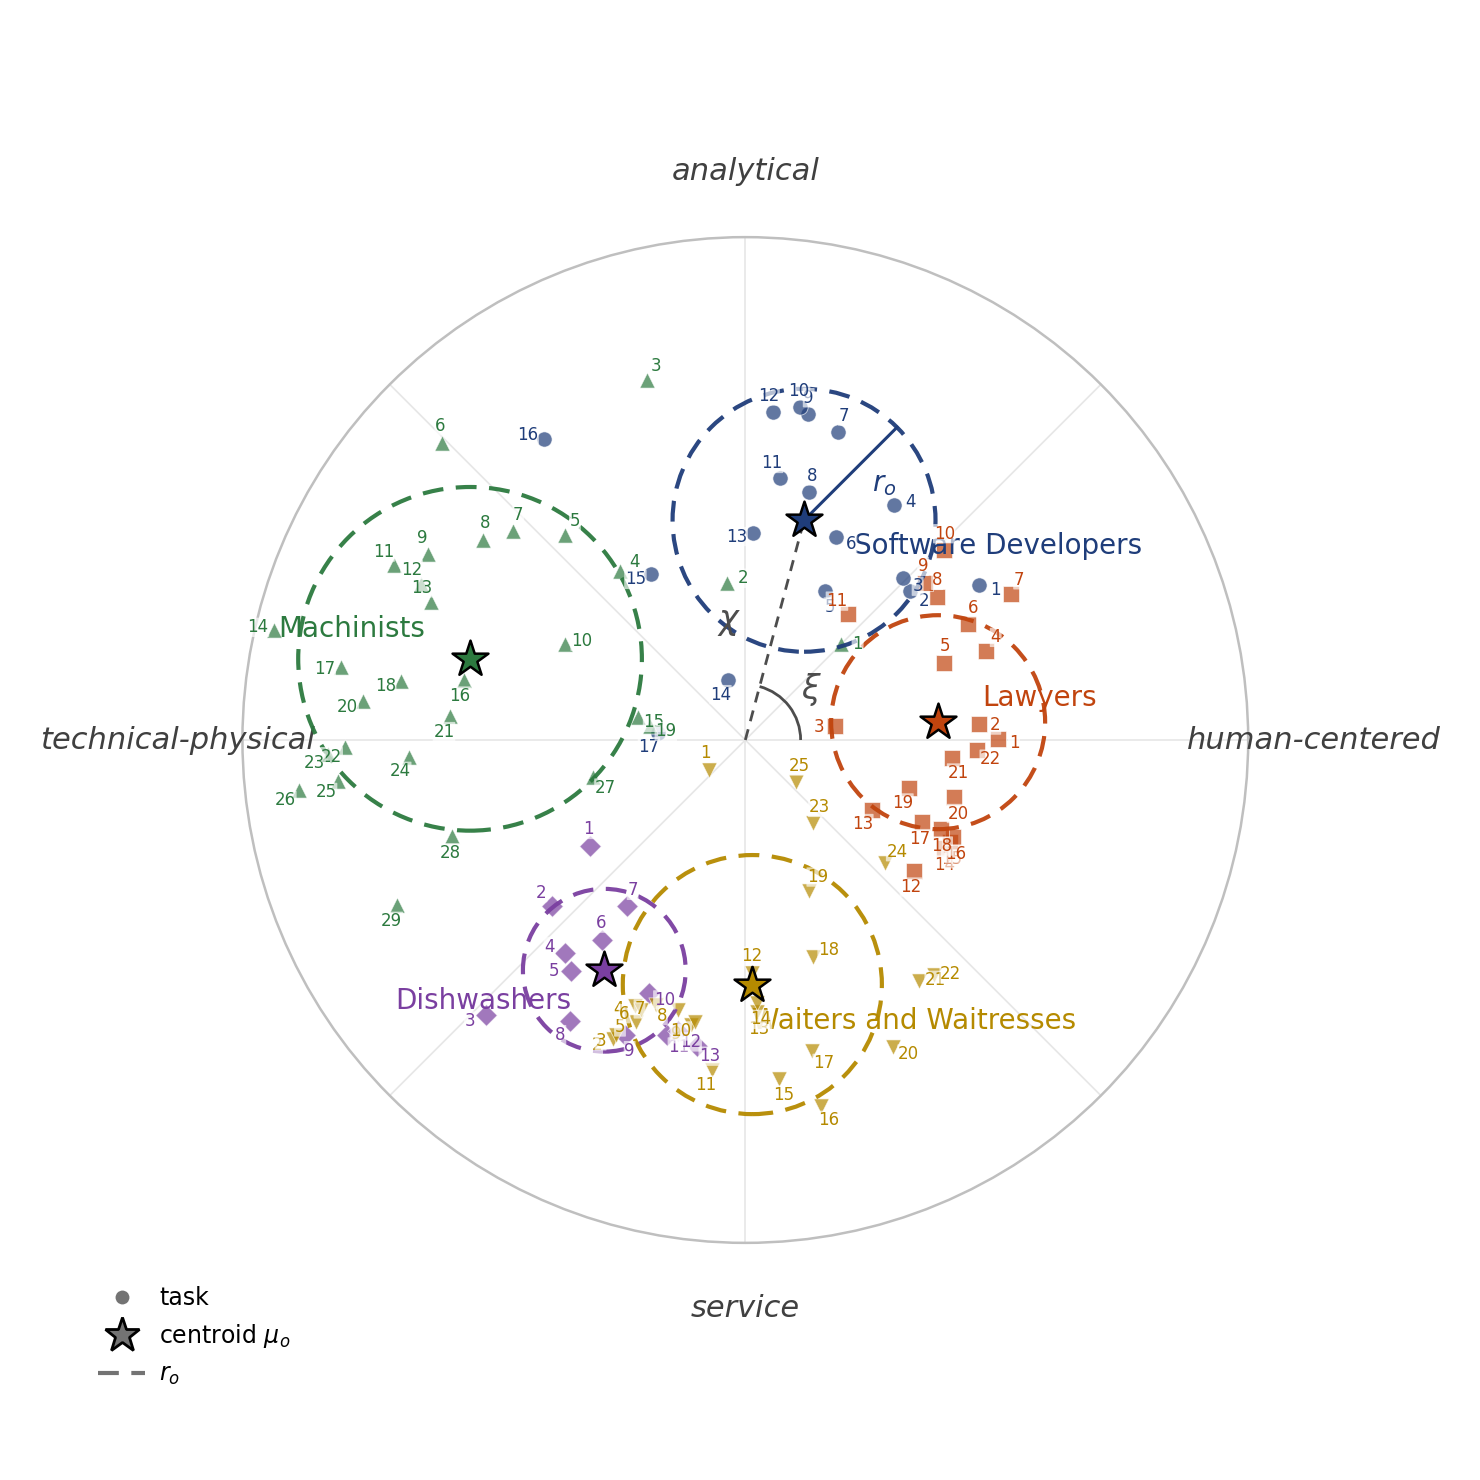
\includegraphics[width=0.9\textwidth]{bundle_examples_numbered.png}
\caption{Panel~(b) of Figure~\ref{fig:geometry-map} with each task
numbered. Within each occupation the numbers run from one around the disk
in order of angle and key into Table~\ref{tab:bundle-tasks}.}
\label{fig:bundle-numbered}
\end{figure}

% Auto-generated by scripts/25_bundle_examples_numbered.py.
% Needs \usepackage{longtable} and \usepackage{booktabs}.
\begin{longtable}{@{}r p{0.72\textwidth} l@{}}
\caption{Tasks of the example occupations of Figure~\ref{fig:geometry-map}, keyed to the numbers in the supplementary numbered panel. Direction is the compass sector of the task on the disk.}\label{tab:bundle-tasks}\\
\toprule
No. & Task & Direction \\ \midrule
\endfirsthead
\multicolumn{3}{c}{\tablename\ \thetable\ (continued)}\\
\toprule No. & Task & Direction \\ \midrule
\endhead
\midrule \multicolumn{3}{r}{continued on next page}\\
\endfoot
\bottomrule
\endlastfoot
\multicolumn{3}{@{}l@{}}{\textit{Software Developers}}\\
\addlinespace[2pt]
1 & Consult with customers or other departments on project status, proposals, or technical issues, such as software system design or maintenance. & human-centered \\
2 & Prepare reports or correspondence concerning project specifications, activities, or status. & human-centered \\
3 & Confer with data processing or project managers to obtain information on limitations or capabilities for data processing projects. & analytical \\
4 & Confer with systems analysts, engineers, programmers and others to design systems and to obtain information on project limitations and capabilities, performance requirements and interfaces. & analytical \\
5 & Supervise and assign work to programmers, designers, technologists, technicians, or other engineering or scientific personnel. & analytical \\
6 & Supervise the work of programmers, technologists and technicians and other engineering and scientific personnel. & analytical \\
7 & Analyze user needs and software requirements to determine feasibility of design within time and cost constraints. & analytical \\
8 & Obtain and evaluate information on factors such as reporting formats required, costs, or security needs to determine hardware configuration. & analytical \\
9 & Develop or direct software system testing or validation procedures, programming, or documentation. & analytical \\
10 & Analyze information to determine, recommend, and plan installation of a new system or modification of an existing system. & analytical \\
11 & Determine system performance standards. & analytical \\
12 & Design, develop and modify software systems, using scientific analysis and mathematical models to predict and measure outcomes and consequences of design. & analytical \\
13 & Store, retrieve, and manipulate data for analysis of system capabilities and requirements. & analytical \\
14 & Coordinate installation of software system. & analytical \\
15 & Modify existing software to correct errors, adapt it to new hardware, or upgrade interfaces and improve performance. & analytical \\
16 & Monitor functioning of equipment to ensure system operates in conformance with specifications. & analytical \\
17 & Train users to use new or modified equipment. & technical-physical \\
\addlinespace
\multicolumn{3}{@{}l@{}}{\textit{Lawyers}}\\
\addlinespace[2pt]
1 & Advise clients concerning business transactions, claim liability, advisability of prosecuting or defending lawsuits, or legal rights and obligations. & human-centered \\
2 & Interpret laws, rulings and regulations for individuals and businesses. & human-centered \\
3 & Prepare, draft, and review legal documents, such as wills, deeds, patent applications, mortgages, leases, and contracts. & human-centered \\
4 & Confer with colleagues with specialties in appropriate areas of legal issue to establish and verify bases for legal proceedings. & human-centered \\
5 & Gather evidence to formulate defense or to initiate legal actions by such means as interviewing clients and witnesses to ascertain the facts of a case. & human-centered \\
6 & Evaluate findings and develop strategies and arguments in preparation for presentation of cases. & human-centered \\
7 & Help develop federal and state programs, draft and interpret laws and legislation, and establish enforcement procedures. & human-centered \\
8 & Study Constitution, statutes, decisions, regulations, and ordinances of quasi-judicial bodies to determine ramifications for cases. & human-centered \\
9 & Analyze the probable outcomes of cases, using knowledge of legal precedents. & human-centered \\
10 & Examine legal data to determine advisability of defending or prosecuting lawsuit. & human-centered \\
11 & Search for and examine public and other legal records to write opinions or establish ownership. & analytical \\
12 & Act as agent, trustee, guardian, or executor for businesses or individuals. & human-centered \\
13 & Select jurors, argue motions, meet with judges, and question witnesses during the course of a trial. & human-centered \\
14 & Present and summarize cases to judges and juries. & human-centered \\
15 & Perform administrative and management functions related to the practice of law. & human-centered \\
16 & Supervise legal assistants. & human-centered \\
17 & Negotiate settlements of civil disputes. & human-centered \\
18 & Probate wills and represent and advise executors and administrators of estates. & human-centered \\
19 & Negotiate contractual agreements. & human-centered \\
20 & Prepare legal briefs and opinions, and file appeals in state and federal courts of appeal. & human-centered \\
21 & Present evidence to defend clients or prosecute defendants in criminal or civil litigation. & human-centered \\
22 & Represent clients in court or before government agencies. & human-centered \\
\addlinespace
\multicolumn{3}{@{}l@{}}{\textit{Machinists}}\\
\addlinespace[2pt]
1 & Advise clients about the materials being used for finished products. & analytical \\
2 & Confer with engineering, supervisory, or manufacturing personnel to exchange technical information. & analytical \\
3 & Test experimental models under simulated operating conditions, for purposes such as development, standardization, or feasibility of design. & analytical \\
4 & Confer with numerical control programmers to check and ensure that new programs or machinery will function properly and that output will meet specifications. & analytical \\
5 & Evaluate machining procedures and recommend changes or modifications for improved efficiency or adaptability. & analytical \\
6 & Measure, examine, or test completed units to check for defects and ensure conformance to specifications, using precision instruments, such as micrometers. & technical-physical \\
7 & Design fixtures, tooling, or experimental parts to meet special engineering needs. & technical-physical \\
8 & Study sample parts, blueprints, drawings, or engineering information to determine methods or sequences of operations needed to fabricate products. & technical-physical \\
9 & Calculate dimensions or tolerances, using instruments, such as micrometers or vernier calipers. & technical-physical \\
10 & Program computers or electronic instruments, such as numerically controlled machine tools. & technical-physical \\
11 & Operate equipment to verify operational efficiency. & technical-physical \\
12 & Diagnose machine tool malfunctions to determine need for adjustments or repairs. & technical-physical \\
13 & Support metalworking projects from planning and fabrication through assembly, inspection, and testing, using knowledge of machine functions, metal properties, and mathematics. & technical-physical \\
14 & Dismantle machines or equipment, using hand tools or power tools to examine parts for defects and replace defective parts where needed. & technical-physical \\
15 & Prepare working sketches for the illustration of product appearance. & technical-physical \\
16 & Monitor the feed and speed of machines during the machining process. & technical-physical \\
17 & Install experimental parts or assemblies, such as hydraulic systems, electrical wiring, lubricants, or batteries into machines or mechanisms. & technical-physical \\
18 & Check work pieces to ensure that they are properly lubricated or cooled. & technical-physical \\
19 & Dispose of scrap or waste material in accordance with company policies and environmental regulations. & technical-physical \\
20 & Install repaired parts into equipment or install new equipment. & technical-physical \\
21 & Establish work procedures for fabricating new structural products, using a variety of metalworking machines. & technical-physical \\
22 & Set up or operate metalworking, brazing, heat-treating, welding, or cutting equipment. & technical-physical \\
23 & Set up, adjust, or operate basic or specialized machine tools used to perform precision machining operations. & technical-physical \\
24 & Maintain machine tools in proper operational condition. & technical-physical \\
25 & Machine parts to specifications, using machine tools, such as lathes, milling machines, shapers, or grinders. & technical-physical \\
26 & Fit and assemble parts to make or repair machine tools. & technical-physical \\
27 & Separate scrap waste and related materials for reuse, recycling, or disposal. & technical-physical \\
28 & Lay out, measure, and mark metal stock to display placement of cuts. & technical-physical \\
29 & Align and secure holding fixtures, cutting tools, attachments, accessories, or materials onto machines. & technical-physical \\
\addlinespace
\multicolumn{3}{@{}l@{}}{\textit{Dishwashers}}\\
\addlinespace[2pt]
1 & Clean garbage cans with water or steam. & technical-physical \\
2 & Wash dishes, glassware, flatware, pots, or pans, using dishwashers or by hand. & technical-physical \\
3 & Transfer supplies or equipment between storage and work areas, by hand or using hand trucks. & service \\
4 & Clean or prepare various foods for cooking or serving. & service \\
5 & Sweep or scrub floors. & service \\
6 & Place clean dishes, utensils, or cooking equipment in storage areas. & service \\
7 & Maintain kitchen work areas, equipment, or utensils in clean and orderly condition. & service \\
8 & Load or unload trucks that deliver or pick up food or supplies. & service \\
9 & Sort and remove trash, placing it in designated pickup areas. & service \\
10 & Prepare and package individual place settings. & service \\
11 & Stock supplies, such as food or utensils, in serving stations, cupboards, refrigerators, or salad bars. & service \\
12 & Set up banquet tables. & service \\
13 & Receive and store supplies. & service \\
\addlinespace
\multicolumn{3}{@{}l@{}}{\textit{Waiters and Waitresses}}\\
\addlinespace[2pt]
1 & Prepare checks that itemize and total meal costs and sales taxes. & technical-physical \\
2 & Roll silverware, set up food stations, or set up dining areas to prepare for the next shift or for large parties. & service \\
3 & Fill salt, pepper, sugar, cream, condiment, and napkin containers. & service \\
4 & Remove dishes and glasses from tables or counters, and take them to kitchen for cleaning. & service \\
5 & Perform cleaning duties, such as sweeping and mopping floors, vacuuming carpet, tidying up server station, taking out trash, or checking and cleaning bathroom. & service \\
6 & Prepare tables for meals, including setting up items such as linens, silverware, and glassware. & service \\
7 & Prepare hot, cold, and mixed drinks for patrons, and chill bottles of wine. & service \\
8 & Clean tables or counters after patrons have finished dining. & service \\
9 & Perform food preparation duties, such as preparing salads, appetizers, and cold dishes, portioning desserts, and brewing coffee. & service \\
10 & Garnish and decorate dishes in preparation for serving. & service \\
11 & Stock service areas with supplies such as coffee, food, tableware, and linens. & service \\
12 & Bring wine selections to tables with appropriate glasses, and pour the wines for customers. & service \\
13 & Write patrons' food orders on order slips, memorize orders, or enter orders into computers for transmittal to kitchen staff. & service \\
14 & Serve food or beverages to patrons, and prepare or serve specialty dishes at tables as required. & service \\
15 & Take orders from patrons for food or beverages. & service \\
16 & Escort customers to their tables. & service \\
17 & Assist host or hostess by answering phones to take reservations or to-go orders, and by greeting, seating, and thanking guests. & service \\
18 & Collect payments from customers. & service \\
19 & Explain how various menu items are prepared, describing ingredients and cooking methods. & service \\
20 & Inform customers of daily specials. & service \\
21 & Present menus to patrons and answer questions about menu items, making recommendations upon request. & service \\
22 & Provide guests with information about local areas, including directions. & service \\
23 & Check with customers to ensure that they are enjoying their meals, and take action to correct any problems. & service \\
24 & Describe and recommend wines to customers. & human-centered \\
25 & Check patrons' identification to ensure that they meet minimum age requirements for consumption of alcoholic beverages. & human-centered \\
\end{longtable}


\clearpage
\section{Notation}
\label{app:notation}

Symbols are collected below, grouped by role.

\begin{longtable}{@{}l >{\raggedright\arraybackslash}p{0.67\textwidth}@{}}
\toprule
Symbol & Meaning \\
\midrule
\endfirsthead
\toprule
Symbol & Meaning \\
\midrule
\endhead
\midrule
\multicolumn{2}{r}{\footnotesize continued on next page} \\
\endfoot
\bottomrule
\endlastfoot

\multicolumn{2}{@{}l}{\textit{Task space and the price field}} \\
\addlinespace
$\mathbf{r}=(\xi,\chi)$ & point in task space; $\xi$ angular, $\chi$ radial coordinate ($\chi=0$ centre, rim $\chi=1$) \\
$\mu_o=\int \mathbf{r}\,b_o(\mathbf{r})\,d\mathbf{r}$ & centroid of occupation $o$'s task bundle $b_o$ \\
$\Delta\mu_o$ & shift of the centroid under the technology shock \\
$d(o,o')=\lVert\mu_o-\mu_{o'}\rVert$ & task-space distance between occupations \\
$\Pi(\mathbf{r})$ & price field: price of capability content at $\mathbf{r}$ (reduced form, estimated from wages) \\
$\nabla\ln\Pi$ & gradient of the log price field \\
$\Pi_{\mathrm{eff}}=e^{\omega_g}\Pi$ & wedge-adjusted price entering the adoption gate (Section~\ref{sec:gate-wedge}) \\
$\widehat{\Delta\ln\Pi}_o=\Delta\mu_o\cdot\nabla\ln\Pi$ & predicted directional wage pressure: first-order log-price change the shift implies (Section~\ref{sec:directional-check}) \\
\addlinespace
\multicolumn{2}{@{}l}{\textit{Capabilities}} \\
\addlinespace
$\mathcal{K}$, $k$ & set of capability clusters and a generic cluster \\
$q_k(\mathbf{r})$, $q_{o,k}$ & level of capability $k$ at $\mathbf{r}$; occupation $o$'s content \\
$v_k$ & weight of capability $k$ in the price functional (the gate weights, $v_k\geq 0$) \\
$v_o$, $\bar v$, $\bar v_k$ & occupation $o$'s capability profile and the mean profile (eq.~\eqref{eq:capability-plane}); $\bar v_k$ the cluster plane mean (eq.~\eqref{eq:capability-field}). Unrelated to the gate weights $v_k$ despite the shared letter \\
$p_k$, $\kappa$ & per-capability price and intercept in $\ln\Pi=\kappa+\sum_k p_k q_k$ \\
\addlinespace
\multicolumn{2}{@{}l}{\textit{Technology field and takeover}} \\
\addlinespace
$K$ & a technology field (cognitive or robot) \\
$z_K,\,A_K$ & reach and amplitude of the field (calibration) \\
$s_K,\,\phi_K(\mathbf{r})$ & replacing share of the field's effectiveness ($s_K=1$ all replacing, $0$ augmenting); $\phi_K$ technical exposure at $\mathbf{r}$ \\
$a(\mathbf{r})$ & operated (takeover) share at $\mathbf{r}$ \\
$R,\,\tau$ & automation cost threshold (takeover compares $\Pi$ to $R/(s_K\phi_K)$) and margin width \\
$D_o$ & displaced share of occupation $o$ \\
$\iota_o(\mathbf{r})$, $B_o=\int\iota_o\,d\mathbf{r}$ & reinstatement inflow and reinstated mass \\
$\gamma$ & reinstatement fraction ($=0.5$) \\
$\hat g(\mathbf{r})$, $M$, $\zeta(\mathbf{r})=M\hat g(\mathbf{r})$ & normalized boundary density (eq.~\eqref{eq:gradient-phi}), seeded task mass $M=\gamma\Delta\Gamma^D$, and seeded density \\
$\delta_o(\mathbf{r})$, $\bar\delta_o(\mathbf{r})$ & priced capability deficit (eq.~\eqref{eq:deficit}) and surplus of occupation $o$ at $\mathbf{r}$ \\
$e_o(\mathbf{r})$ & readiness to attach (eq.~\eqref{eq:attachment}) \\
$C(\mathbf{r})=\sum_o L_o e_o(\mathbf{r})$ & attachment capacity at $\mathbf{r}$ \\
$u(\mathbf{r})$ & unbound task density (eq.~\eqref{eq:unbound}) \\
$\beta$ & congestion exponent in $V(\mathbf{r})=\Pi\,n^{\beta}$; human task-work is paid its marginal value product out of $\beta V$, capital is paid its cost, $(1-\beta)V$ is the congestion rent to the fixed factor \\
$\Phi(C)=C/(1+C)$ & bound fraction at congestion $C$ \\
$\Delta w_o$ & bundle wage change of occupation $o$ (eq.~\eqref{eq:wage-change}) \\
\addlinespace
\multicolumn{2}{@{}l}{\textit{Wages and rents}} \\
\addlinespace
$w_{\mathrm{obs},o},\,w_{\mathrm{bundle},o}$ & observed wage and model bundle wage of occupation $o$ \\
$\omega_o=\ln w_{\mathrm{obs},o}-\ln w_{\mathrm{bundle},o}$ & wage residual of occupation $o$ against its bundle priced at the field \\
$\omega_g$ & family wage wedge: the job-family mean of $\omega_o$ (Section~\ref{sec:gate-wedge}) \\
\addlinespace
\multicolumn{2}{@{}l}{\textit{Equilibrium and mobility}} \\
\addlinespace
$n(\mathbf{r})$ & total task-work density (eq.~\eqref{eq:taskwork-density}) \\
$H(\mathbf{r})=\sum_o L_o h_o(\mathbf{r})$ & human task-work density \\
$V(\mathbf{r})$ & place output (eq.~\eqref{eq:place-output}) \\
$W_o$ & occupation value (eq.~\eqref{eq:occ-value}); the object workers sort on \\
$\Lambda$ & labour share of variable task-work income (eq.~\eqref{eq:labour-share}) \\
$\ell$ & acquisition scale in the readiness $e_o$ (eq.~\eqref{eq:attachment}) \\
$L_0,\,L$ & baseline and re-solved employment allocation \\
$\lambda$ & cognitive demand-shifter exponent in the assignment closure (Appendix~\ref{app:assignment}) \\
$c_m,\,\nu$ & mobility cost and logit smoothness in the re-sorting map \\
$\alpha_o$ & anchoring constants in the re-sorting map; observed employment is the zero-technology fixed point \\
$\rho,\,\lambda_{\mathrm{over}}$ & attachment locality scale and over-qualification weight (eq.~\eqref{eq:attachment}) \\
\end{longtable}

\end{document}
